\chapter{Results Of Testing On Various Cases}
To evaluate the performance of the CPR implementation on \texttt{UTCOMPRS}, six compositional cases were run. 
The first three cases were originally presented in \cite{fernandes}, in an Adaptive-Implicit study in \texttt{UTCOMPRS}. 
The first case (\texttt{Case 1}) is a three-phase model that involves gas injection and aimed 
at testing the effects of dispersion. The second case (\texttt{Case 2}) is a gas-flooding model in 
a heterogeneous reservoir. The third case (\texttt{Case 3}) is a four-phase $CO_{2}$ flooding model 
in an areal heterogeneous reservoir. The fourth case (\texttt{Case 4}) is an extension of the third case to 3D. 
These cases are presented below and compared with CPR preconditioner against
the standard solver in \texttt{UTCOMPRS} which is a Krylov based \texttt{GMRES} with \texttt{ILU(0)} as a global
preconditioner. 

\section{Case 1}
The details of the reservoir being simulated are shown in table \ref{case1}. 

\FloatBarrier
\begin{center}
\begin{table}[h!]
\begin{adjustbox}{width=0.8\textwidth}
    \begin{threeparttable}
    \caption{\textbf{Case 1 Reservoir Parameters\supercite{fernandes}.}}
    \label{case1}
        \begin{tabular}{l r }
            \toprule
            Simulatoin Parameters & Value\\
            \midrule
	\rowcolor{red!20}\textit{\textbf{Reservoir data}}      & \\
	Grid:      &           $160\times160\times10$ ($256,000$ active) \\
	\rowcolor{blue!5}Number of wells:      &  2 (1 injector / 1 producer) \\
	Length, width and thickness:      & $170.69$ m, $170.69$ m and $30.48$ m\\
	\rowcolor{blue!5}Porosity:       &          $0.35$ \\
	Initial water saturation:    & $0.3$ \\      
	\rowcolor{blue!5}Initial pressure:    &      $10.34$ MPa\\
	Formation temperature:    & $344.26$ K     \\
	\rowcolor{blue!5}Tortuosity:    &      $1.0$ \\
	Longitudinal dispersivity (W/O/G):    & $4.74$ m, $4.74$ m, and $4.74$ m\\
	\rowcolor{blue!5}Transversal dispersivity (W/O/G):    & $0.474$ m, $0.474$ m, and $0.474$ m\\
	Gas injection rate:    &       $28,316 \ m^{3}/d$ \\
	\rowcolor{blue!5}Producer’s bottom hole pressure:    &       $8.96$ MPa\\
	Reservoir’s initial composition ($C_{1}$, $C_{3}$, $C_{6}$, $C_{10}$, $C_{15}$ and $C_{20}$): & $0.5$, $0.03$, $0.07$, $0.2$, $0.15$, and $0.05$\\
	\rowcolor{blue!5}Injection fluid composition ($C_{1}$, $C_{3}$, $C_{6}$, $C_{10}$, $C_{15}$ and $C_{20}$):    &   $0.77$, $0.2$, $0.01$, $0.01$, $0.005$, and $0.005$\\
	\rowcolor{red!20}\textit{\textbf{Run data}}    &       \\
	Simulation time (days):    &  $1,000$\\
	\rowcolor{blue!5}Simulation time (pore volumes):    & $0.822$\\
            \bottomrule
        \end{tabular}
    \end{threeparttable}
\end{adjustbox}    
\end{table}
\end{center}
\FloatBarrier

\begin{figure}
\centering
\begin{subfigure}{.5\textwidth}
  \centering
  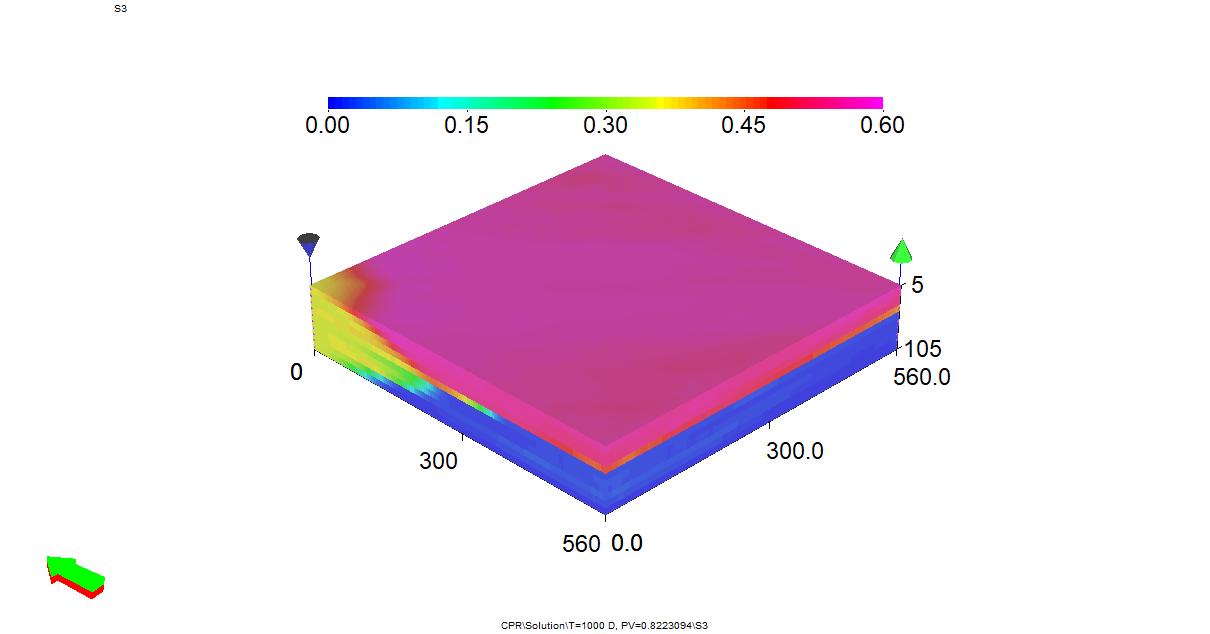
\includegraphics[width=1.3\linewidth]{figures/case1_cpr_sgas.png}
  \caption{\texttt{CPR-AMG} preconditioner.}
\end{subfigure}%
\begin{subfigure}{.5\textwidth}
  \centering
  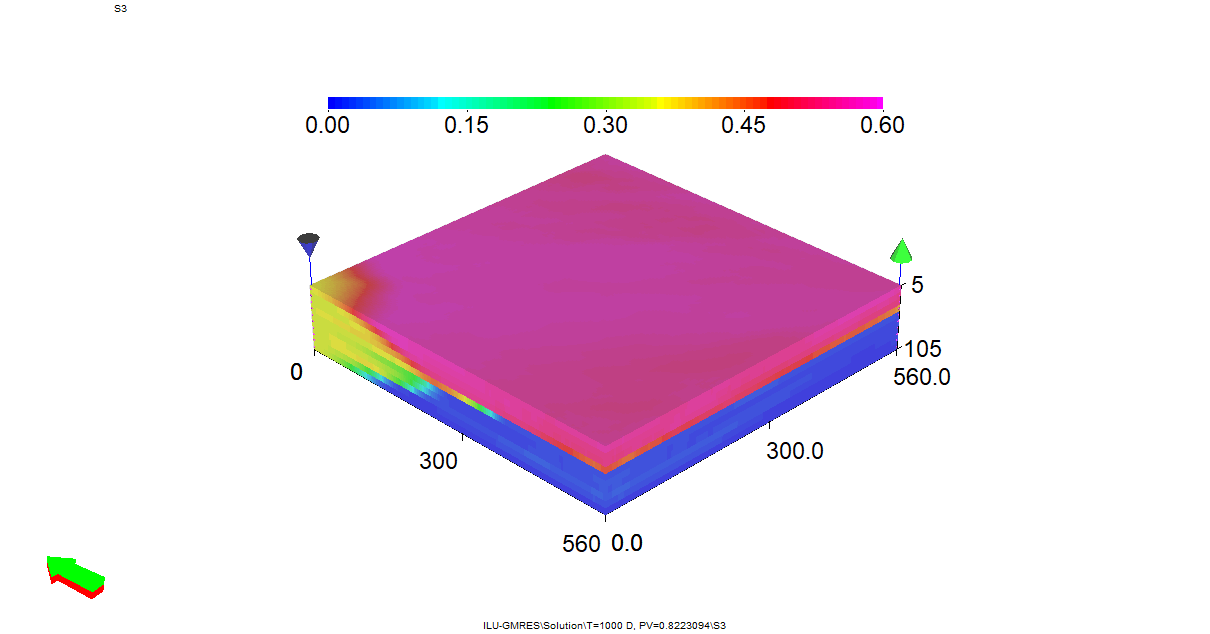
\includegraphics[width=1.3\linewidth]{figures/case1_ilu_sgas.png}
  \caption{\texttt{GMRES-ILU(0)} preconditioner}
\end{subfigure}
\caption{A comparison of \texttt{Case 1} gas saturation $S_{g}$ distribution for the two different preconditioning methods after 1000 days of simulation.}
\label{case1sg}
\end{figure}

\begin{table}[h!]
   \caption{Comparison parameters for \texttt{Case 1}.}
   \label{case1-tab}
   \small
   \centering
   \begin{tabular}{lcc}
   \toprule\toprule
   \textbf{Variable} & \textbf{CPR-AMG} & \textbf{GMRES-ILU(0)} \\
   \midrule
   CPU Time (hr) & 1.26 & 9.4 \\
   Solver Time (hr) & 0.79 & 8.97 \\
   \# Newton Iterations & 147 & 147 \\
   \# Solver Iterations & 4,025 & 107,192 \\
   \# Time Steps & 67 & 67 \\
   \bottomrule
   \end{tabular}
\end{table}

\begin{figure}
\centering
\begin{subfigure}{.5\textwidth}
  \centering
  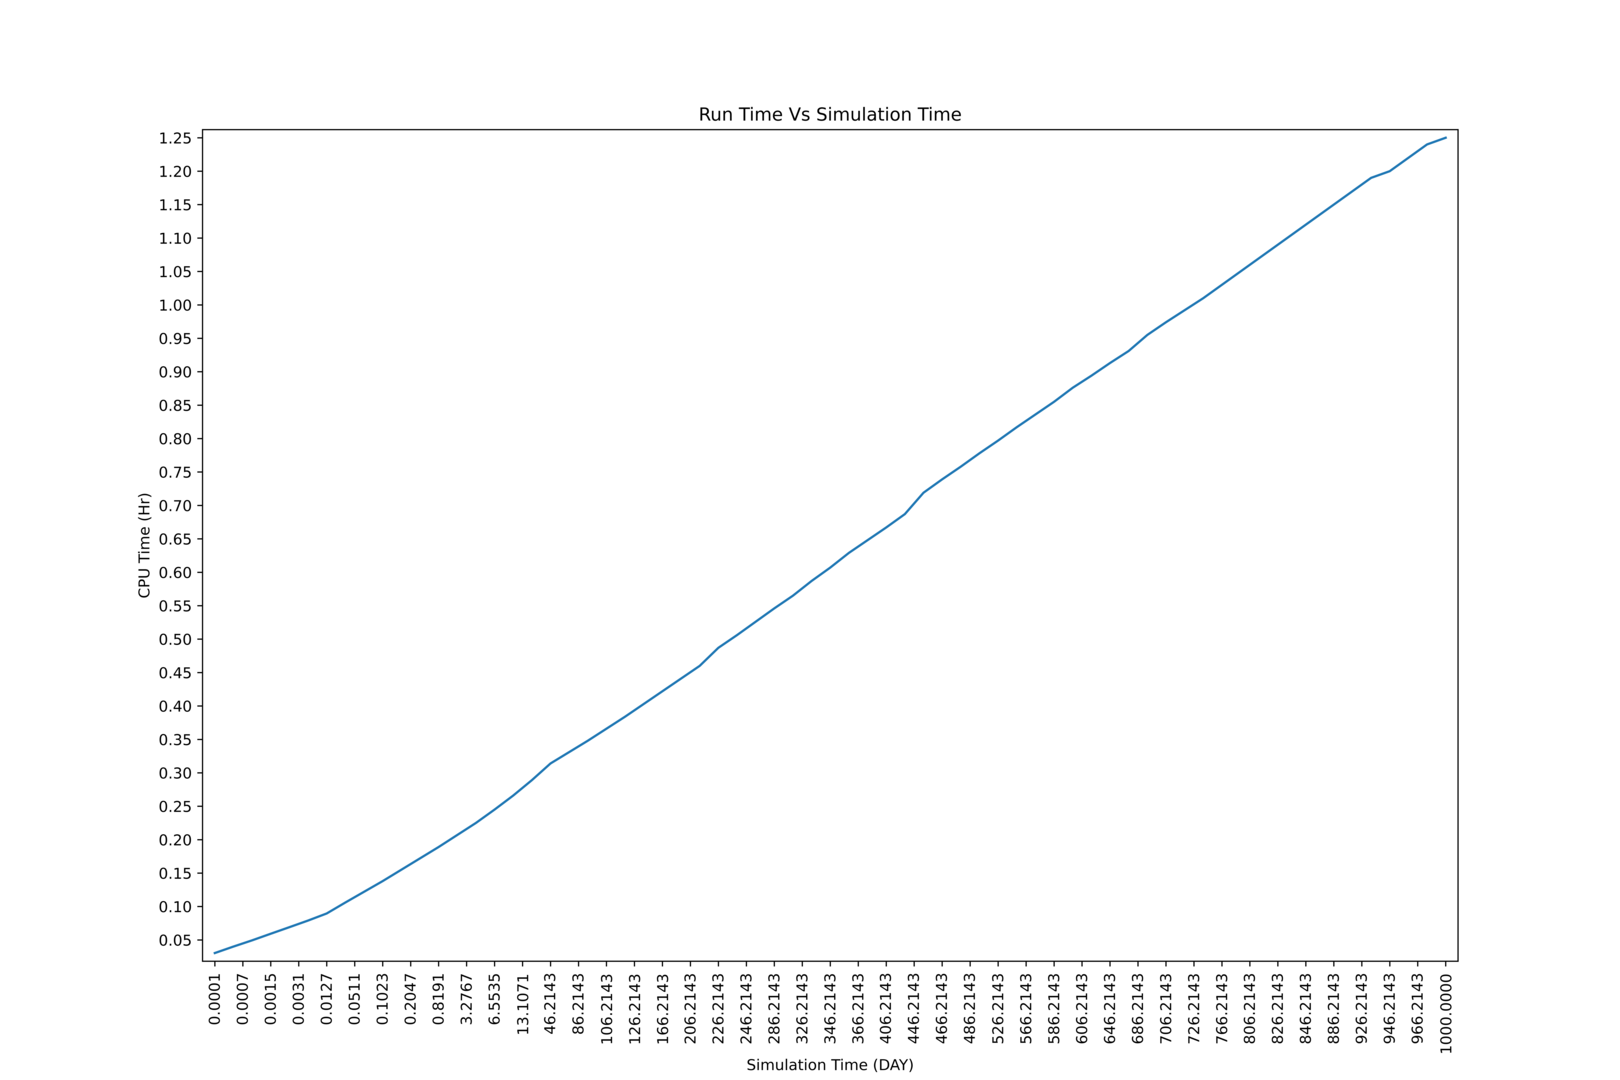
\includegraphics[width=1.1\linewidth]{figures/case1/cpr/cpu_time.png_reduced.png}
  \caption{\texttt{CPR-AMG} preconditioner.}
	\label{case1_cpu_cpr}
\end{subfigure}%
\begin{subfigure}{.5\textwidth}
  \centering
  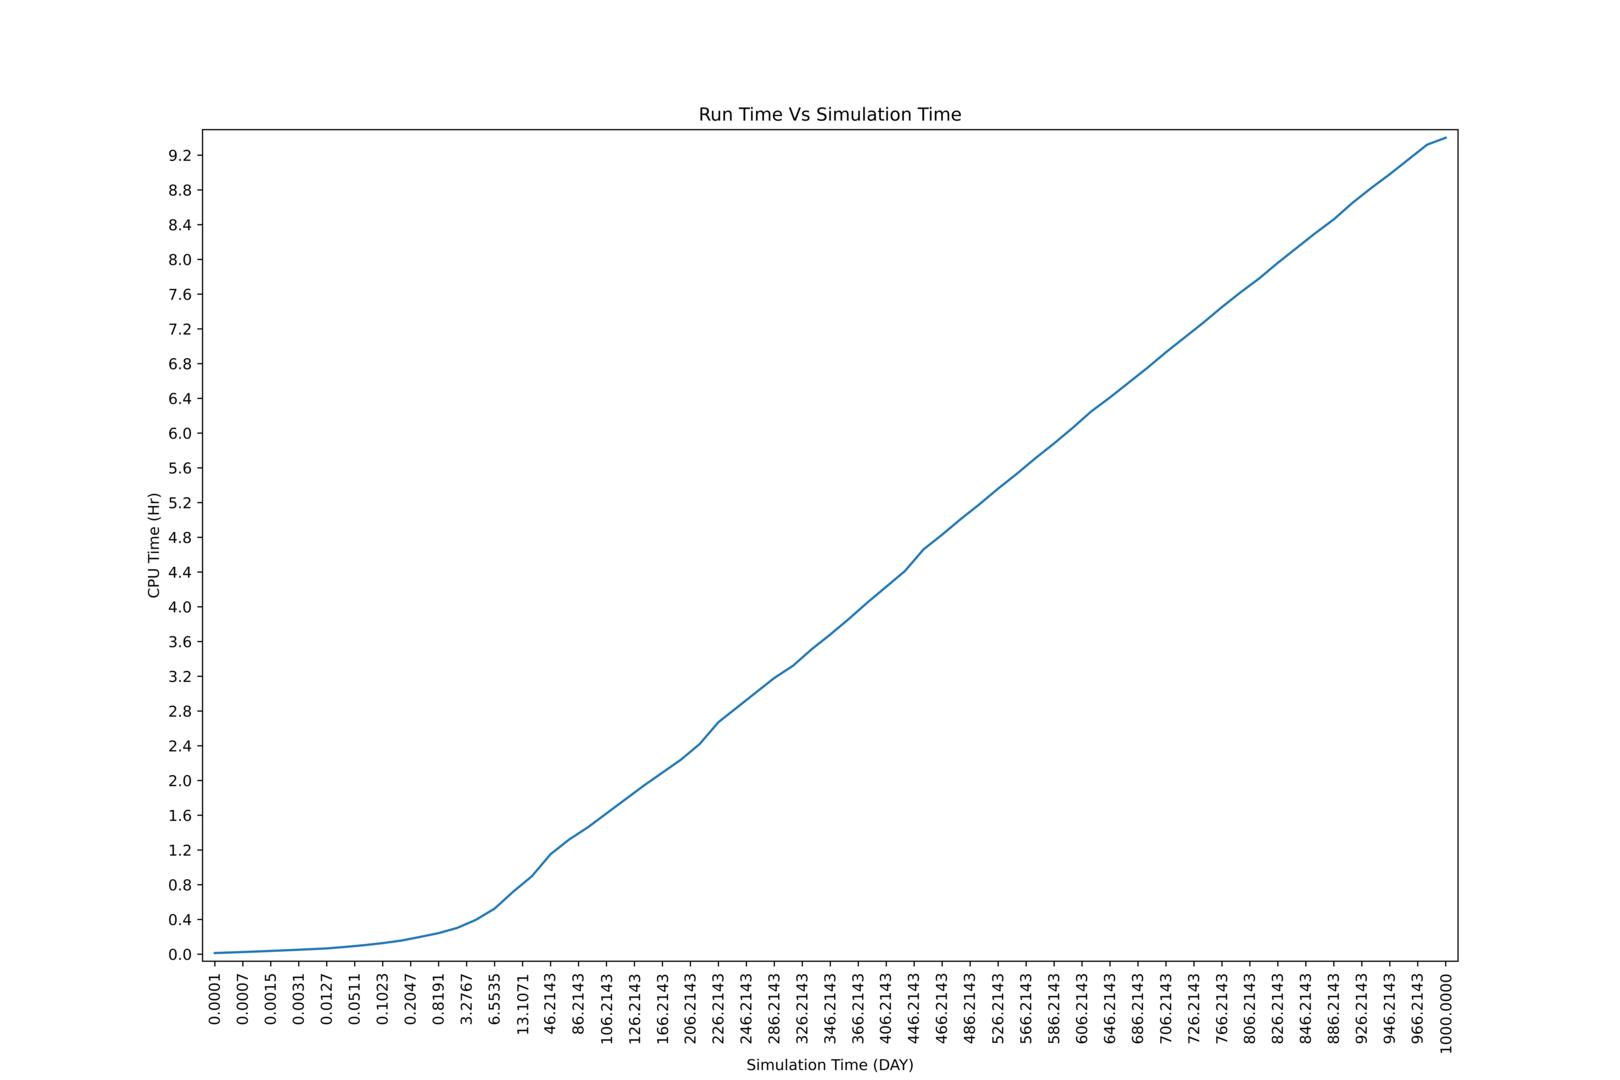
\includegraphics[width=1.1\linewidth]{figures/case1/ilu/cpu_time.png_reduced.png}
  \caption{\texttt{GMRES-ILU(0)} preconditioner}
	\label{case1_cpu_ilu}
\end{subfigure}
\begin{subfigure}{.5\textwidth}
  \centering
  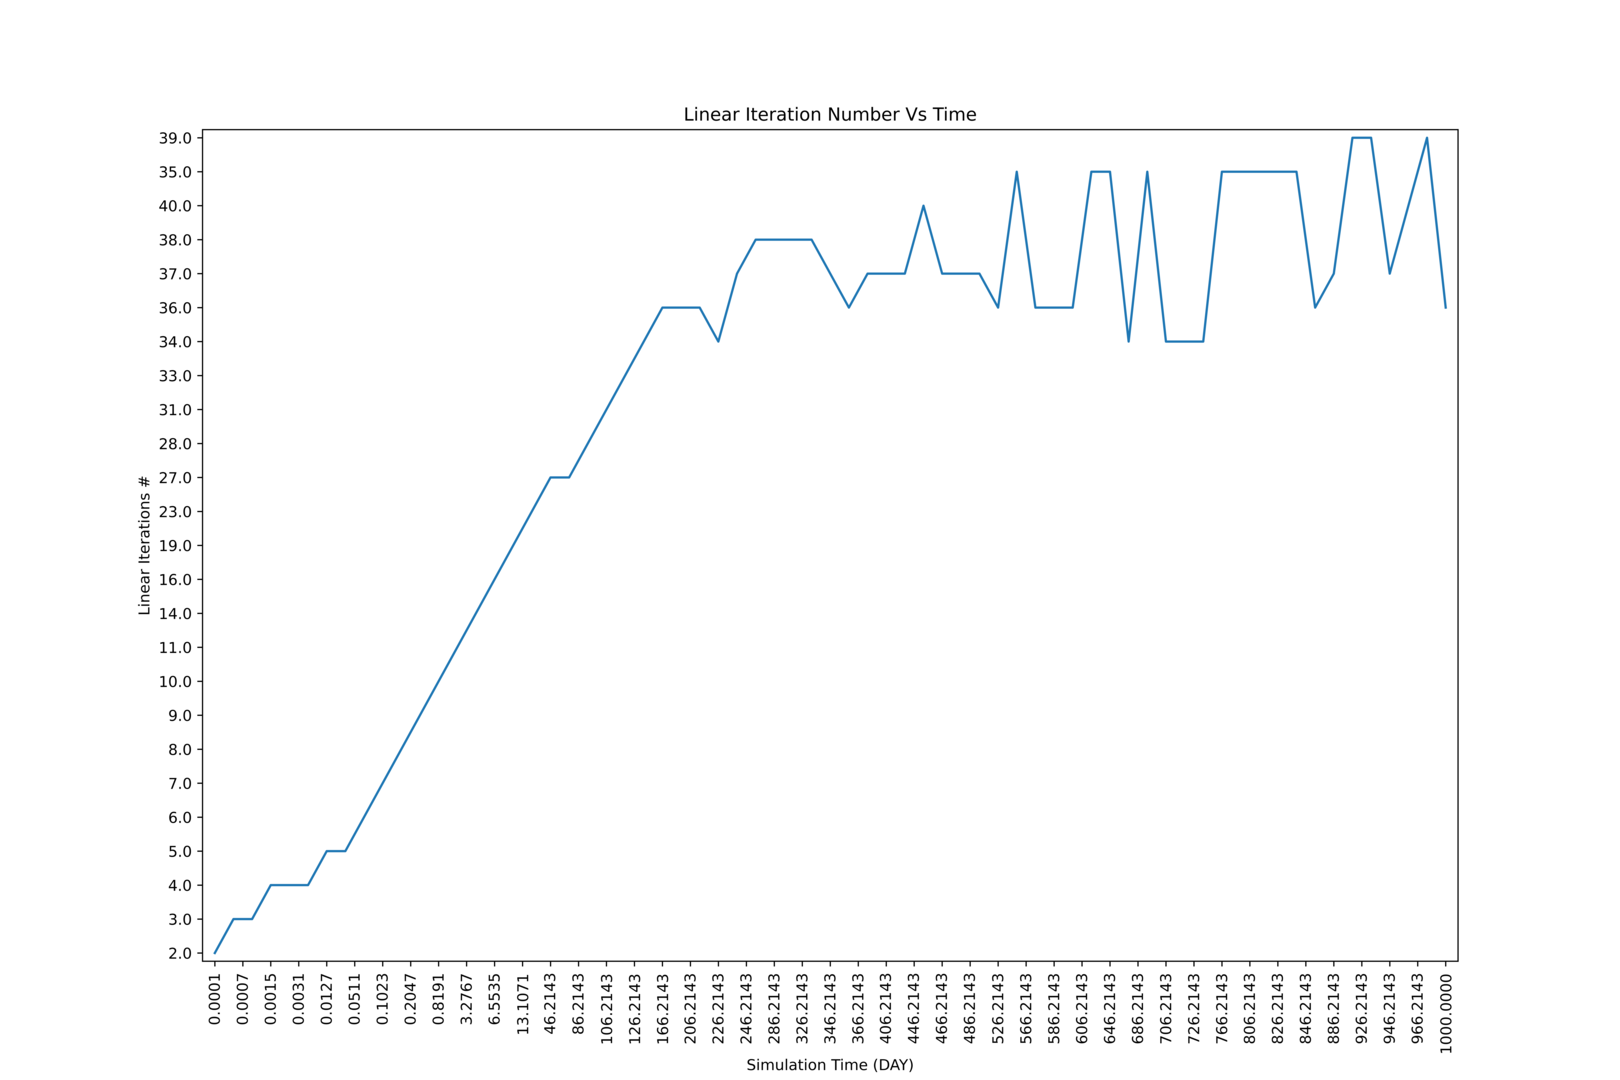
\includegraphics[width=1.1\linewidth]{figures/case1/cpr/its_time.png_reduced.png}
  \caption{\texttt{CPR-AMG} preconditioner.}
	\label{case1_its_cpr}
\end{subfigure}%
\begin{subfigure}{.5\textwidth}
  \centering
  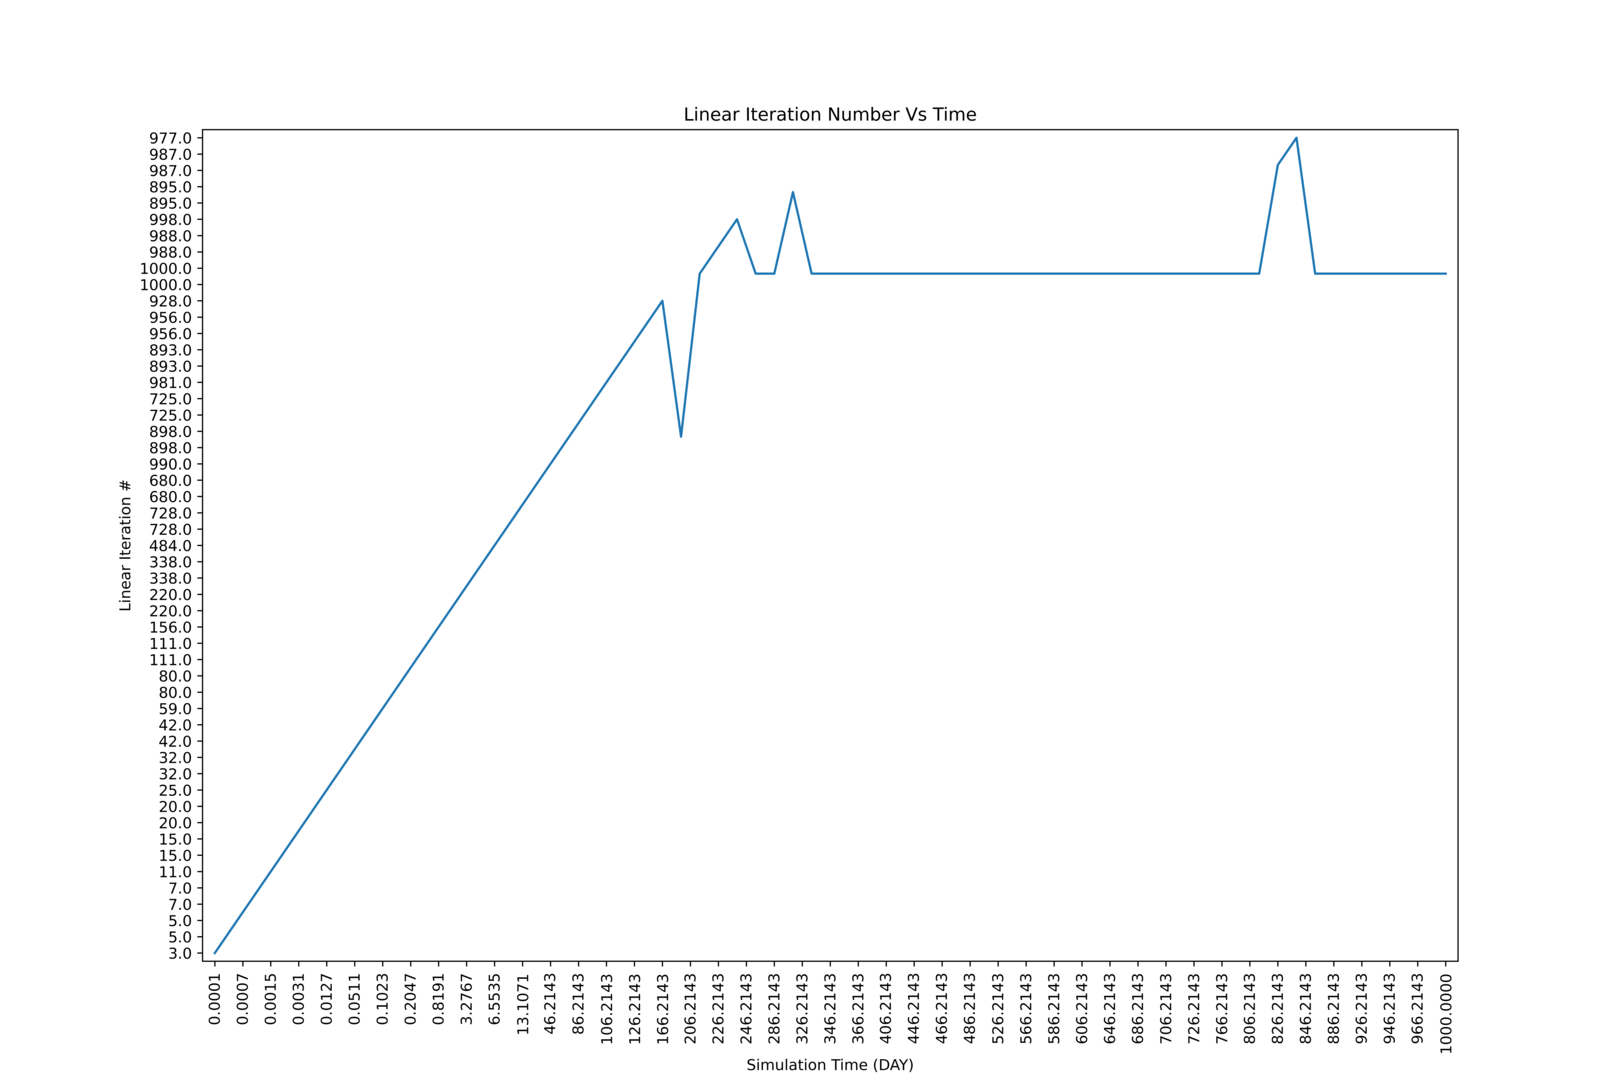
\includegraphics[width=1.1\linewidth]{figures/case1/ilu/its_time.png_reduced.png}
  \caption{\texttt{GMRES-ILU(0)} preconditioner}
	\label{case1_its_ilu}
\end{subfigure}
\begin{subfigure}{.5\textwidth}
  \centering
  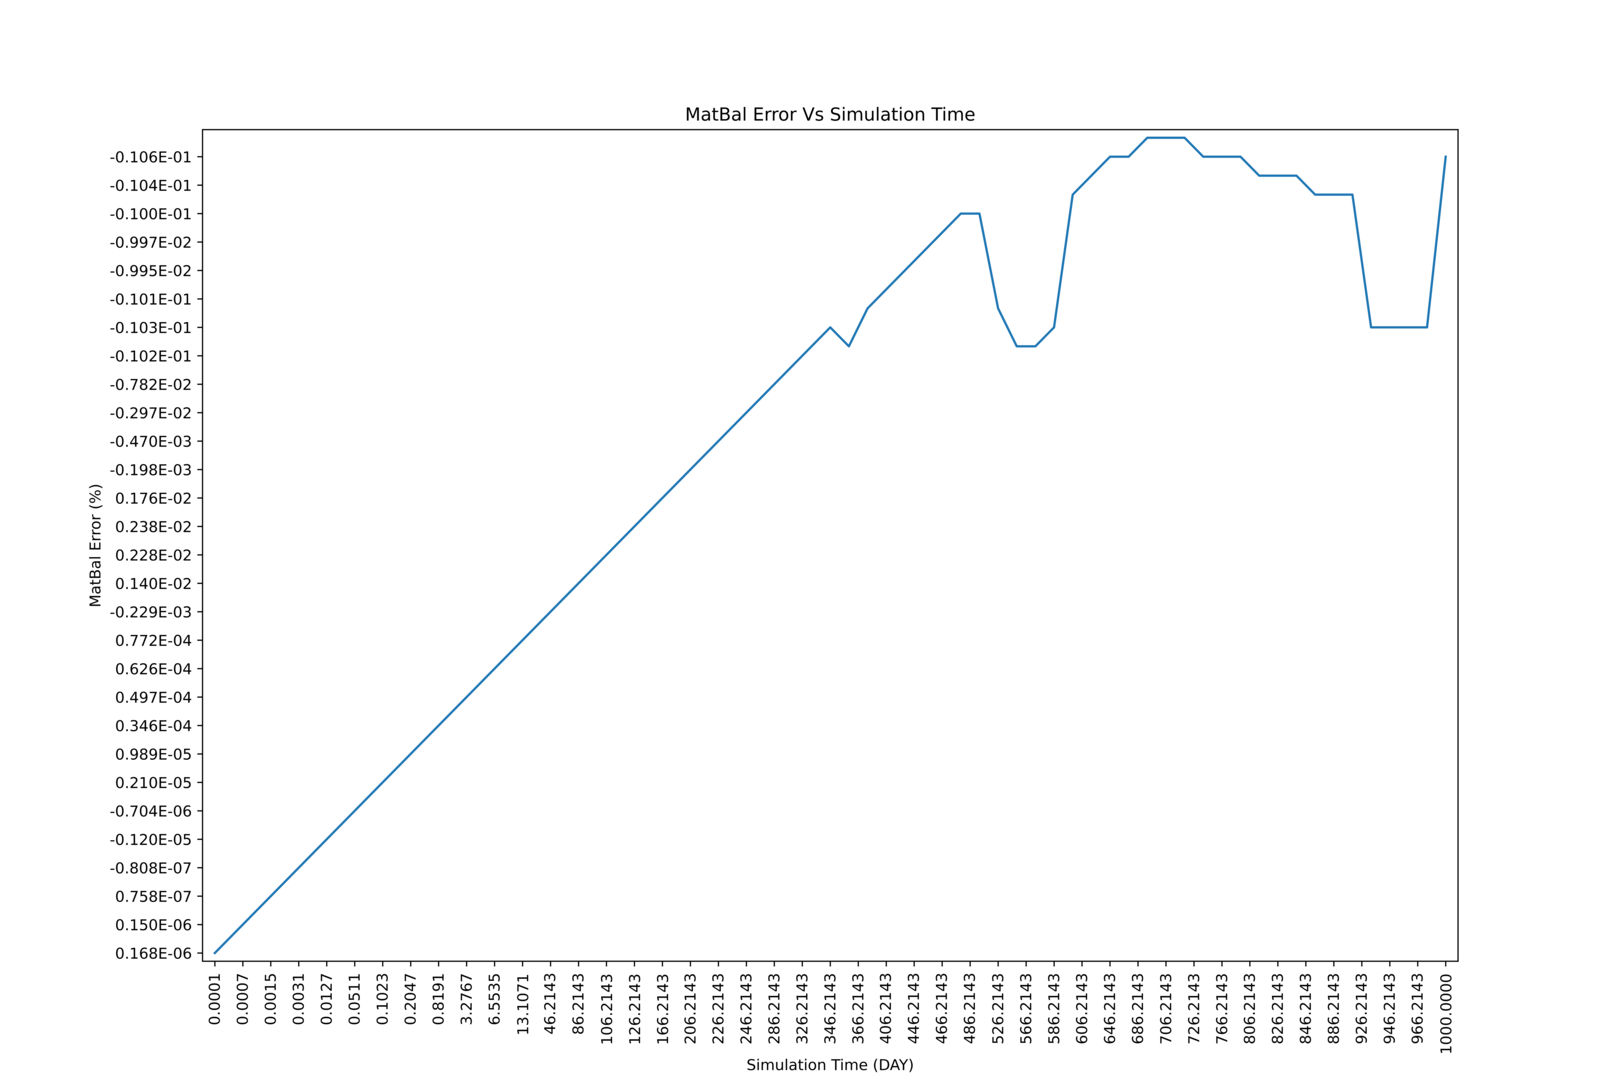
\includegraphics[width=1.1\linewidth]{figures/case1/cpr/matbalerr_time.png_reduced.png}
  \caption{\texttt{CPR-AMG} preconditioner.}
	\label{case1_matbalerr_cpr}
\end{subfigure}%
\begin{subfigure}{.5\textwidth}
  \centering
  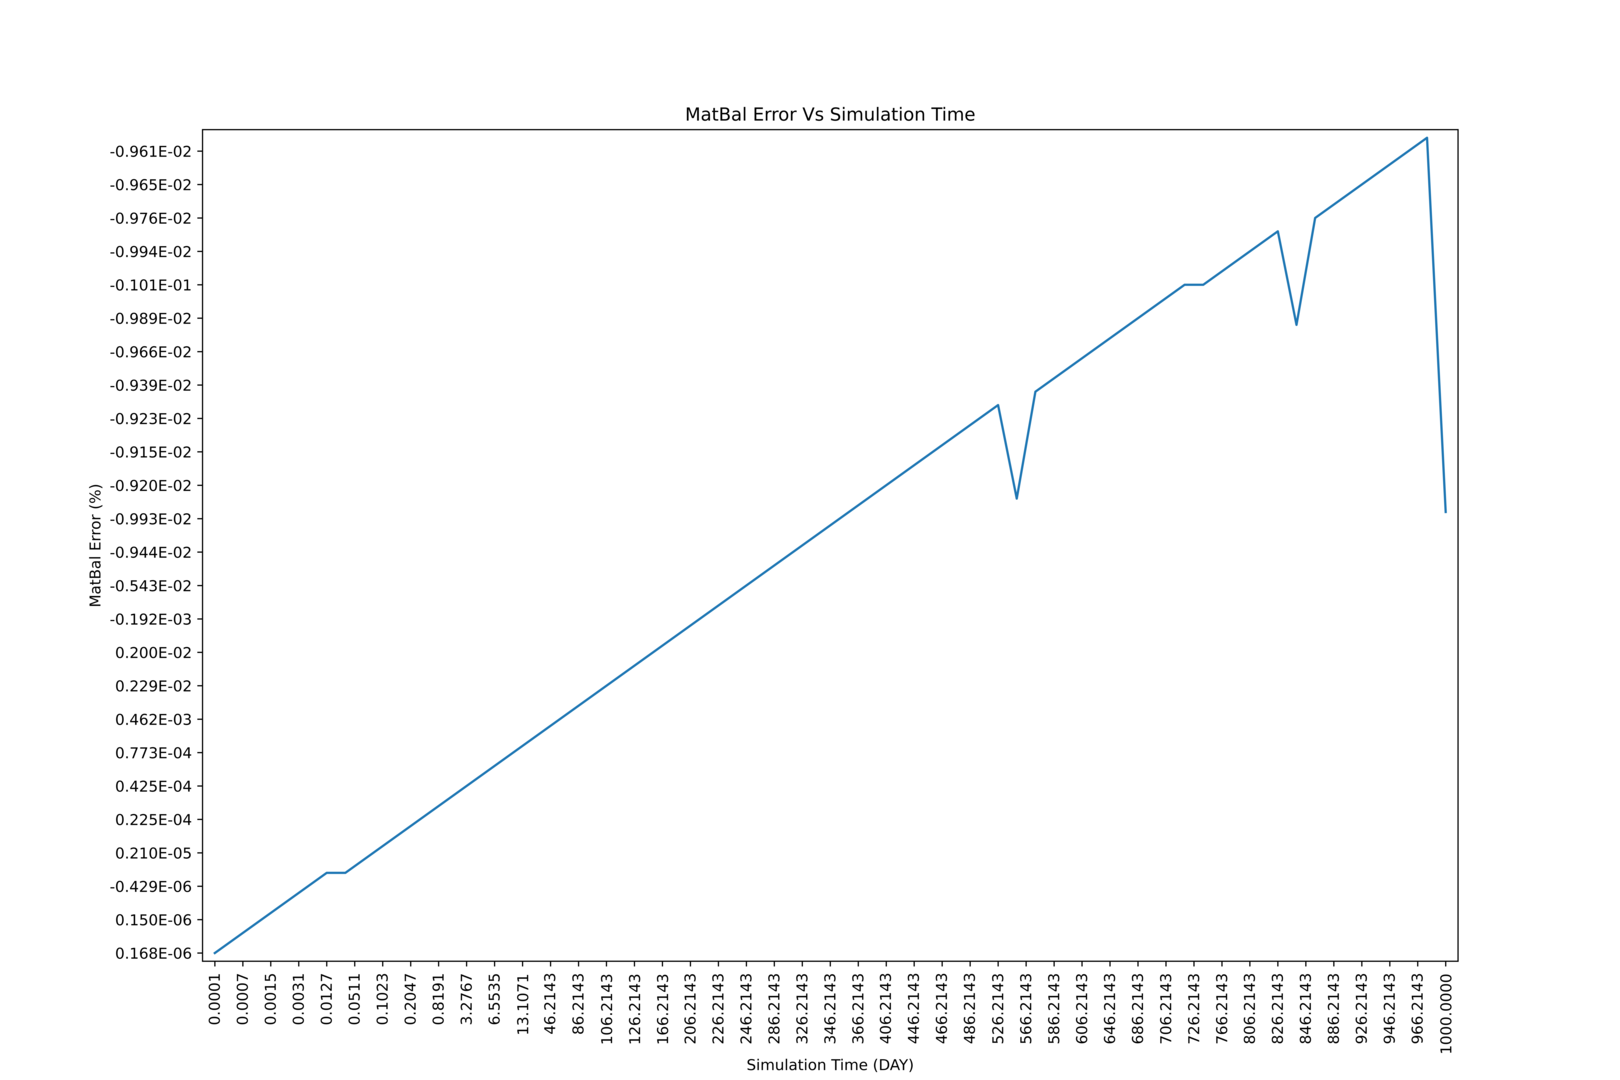
\includegraphics[width=1.1\linewidth]{figures/case1/ilu/matbalerr_time.png_reduced.png}
  \caption{\texttt{GMRES-ILU(0)} preconditioner}
	\label{case1_matbalerr_ilu}
\end{subfigure}
%\caption{A comparison for \texttt{Case 1} for the two different preconditioning methods.}
\caption[caption]{A comparison for \texttt{Case 1} for the two different preconditioning methods.\\\hspace{\textwidth}
		\cref{case1_cpu_cpr,case1_cpu_ilu}: CPU run time against simulation time. \\\hspace{\textwidth}
		\cref{case1_its_cpr,case1_its_ilu}: Linear iterations against simulation time.\\\hspace{\textwidth}
		\cref{case1_matbalerr_cpr,case1_matbalerr_ilu}: Material balance error against simulation time.}
\label{case1_param}
\end{figure}
\clearpage

\section{Case 2}

\FloatBarrier
\begin{center}
\begin{table}[h!]
\begin{adjustbox}{width=0.8\textwidth}
    \begin{threeparttable}
    \caption{\textbf{Case 2 Reservoir Parameters\supercite{fernandes}.}}
    \label{case2}
        \begin{tabular}{l r }
            \toprule
            Simulatoin Parameters & Value\\
            \midrule
	\rowcolor{red!20}\textit{\textbf{Reservoir data}}      & \\
	Grid:      &           $200\times400\times25$ ($465,816$ active) \\
	\rowcolor{blue!5}Number of wells:      &  49 (25 injectors / 24 producers) \\
	Length, width and thickness:      & $1,219.2$ m, $2,438.4$ m and $45.72$ m\\
	Initial water saturation:    & $0.17$ \\      
	\rowcolor{blue!5}Initial pressure:    &      $20.68$ MPa\\
	Formation temperature:    & $303.15$ K     \\
	Gas injection rate:    &       $86,366 \ m^{3}/d$ \\
	\rowcolor{blue!5}Producer’s bottom hole pressure:    &       $20.68$ MPa\\
	Reservoir’s initial composition ($C_{1}$, $C_{3}$ $C_{10}$): & $0.1$, $0.19$, $0.8$\\
	\rowcolor{blue!5}Injection fluid composition ($C_{1}$, $C_{3}$, $C_{10}$):    &   $0.95$, $0.05$, $0.0$\\
	\rowcolor{red!20}\textit{\textbf{Run data}}    &       \\
	Simulation time (days):    &  $2,190$\\
	\rowcolor{blue!5}Simulation time (pore volumes):    & $1.477$\\
            \bottomrule
        \end{tabular}
    \end{threeparttable}
\end{adjustbox}    
\end{table}
\end{center}
\FloatBarrier

\begin{table}[h!]
   \caption{Comparison parameters for \texttt{Case 2}.}
   \label{case2-tab}
   \small
   \centering
   \begin{tabular}{lcc}
   \toprule\toprule
   \textbf{Variable} & \textbf{CPR-AMG} & \textbf{GMRES-ILU(0)} \\
   \midrule
   CPU Time (hr) & 27.5 & 54.2 \\
   Solver Time (hr) & 21.31 & 48.42 \\
   \# Newton Iterations & 5,751 & 5,717 \\
   \# Solver Iterations & 21,821 & 177,798 \\
   \# Time Steps & 624 & 624 \\
   \bottomrule
   \end{tabular}
\end{table}

\begin{figure}
\centering
\begin{subfigure}{.5\textwidth}
  \centering
  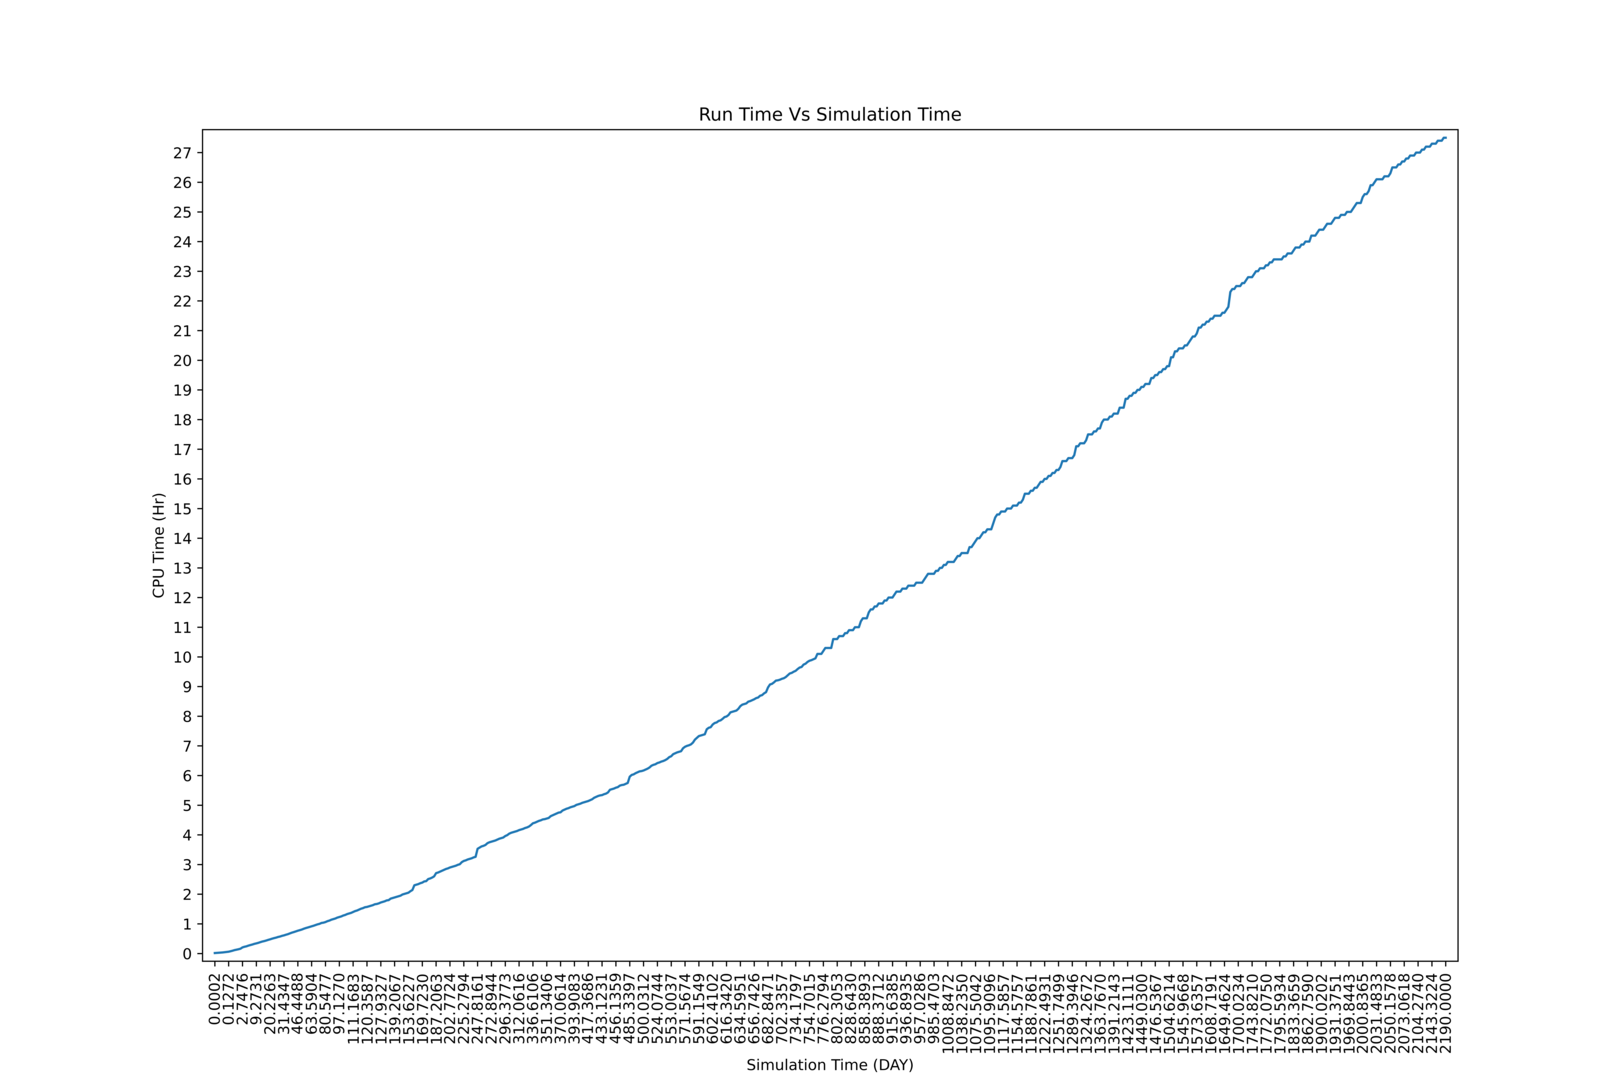
\includegraphics[width=1.1\linewidth]{figures/case2/cpr/cpu_time.png_reduced.png}
  \caption{\texttt{CPR-AMG} preconditioner.}
	\label{case2_cpu_cpr}
\end{subfigure}%
\begin{subfigure}{.5\textwidth}
  \centering
  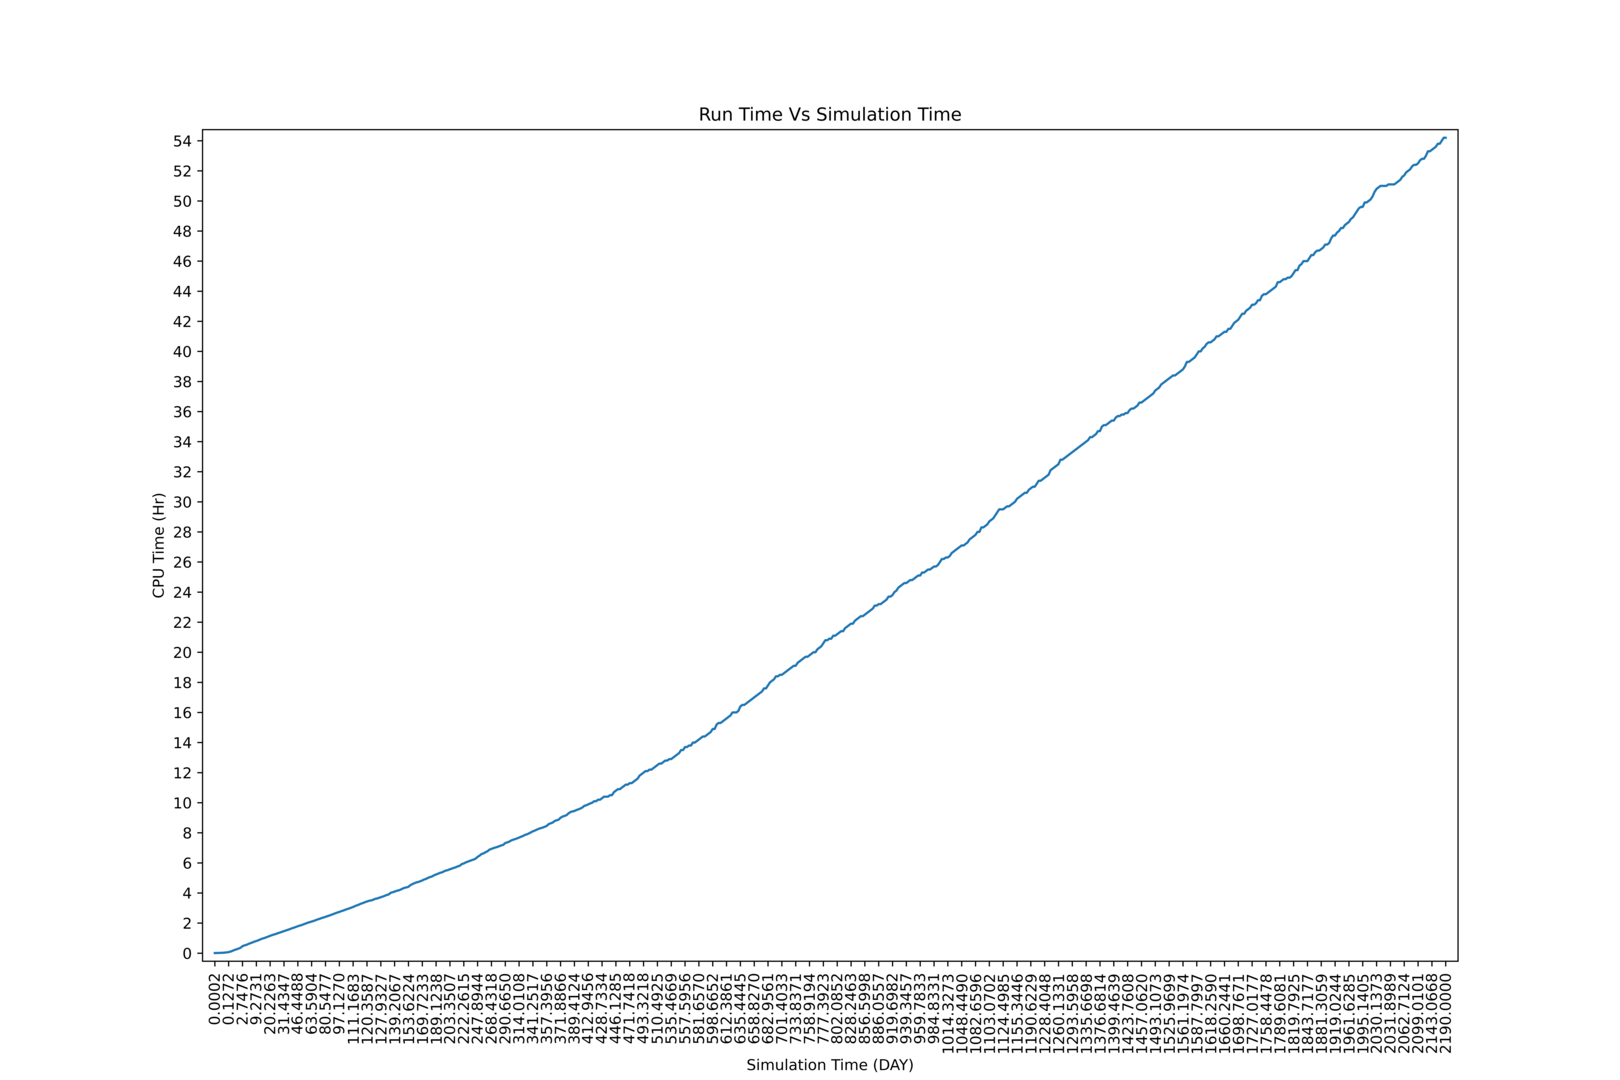
\includegraphics[width=1.1\linewidth]{figures/case2/ilu/cpu_time.png_reduced.png}
  \caption{\texttt{GMRES-ILU(0)} preconditioner}
	\label{case2_cpu_ilu}
\end{subfigure}
\begin{subfigure}{.5\textwidth}
  \centering
  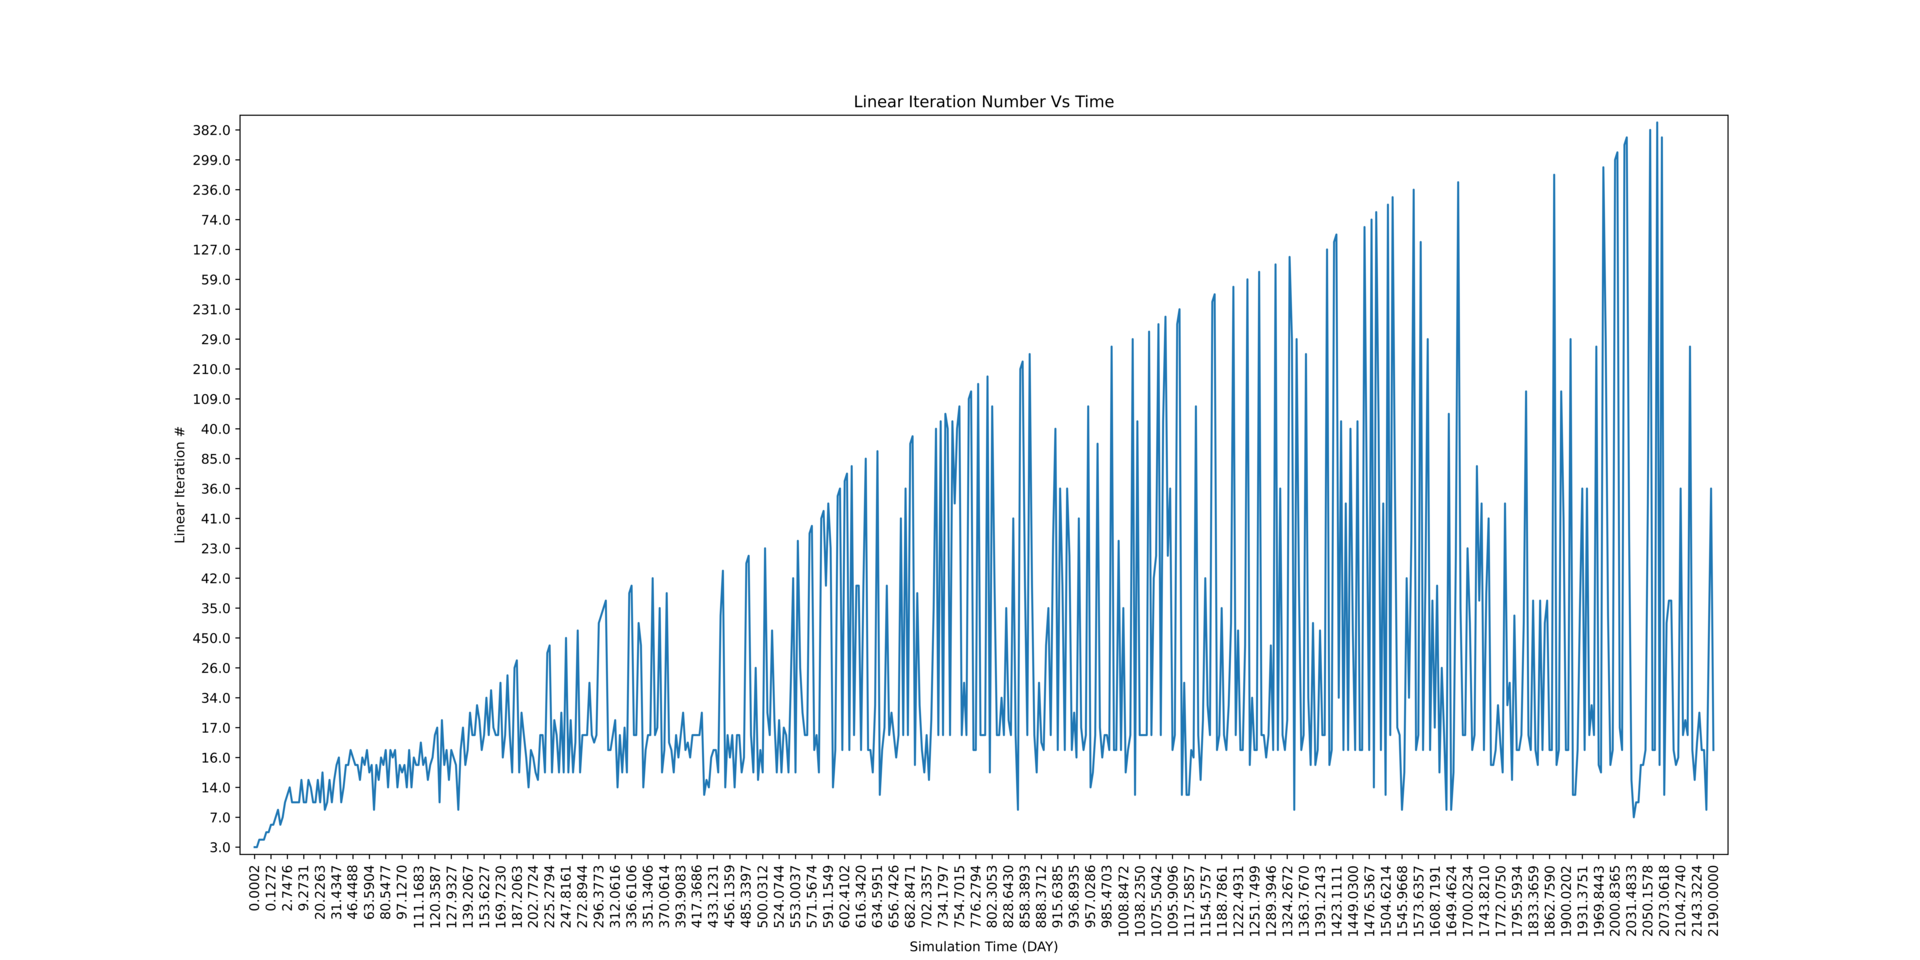
\includegraphics[width=1.1\linewidth]{figures/case2/cpr/its_time.png_reduced.png}
  \caption{\texttt{CPR-AMG} preconditioner.}
	\label{case2_its_cpr}
\end{subfigure}%
\begin{subfigure}{.5\textwidth}
  \centering
  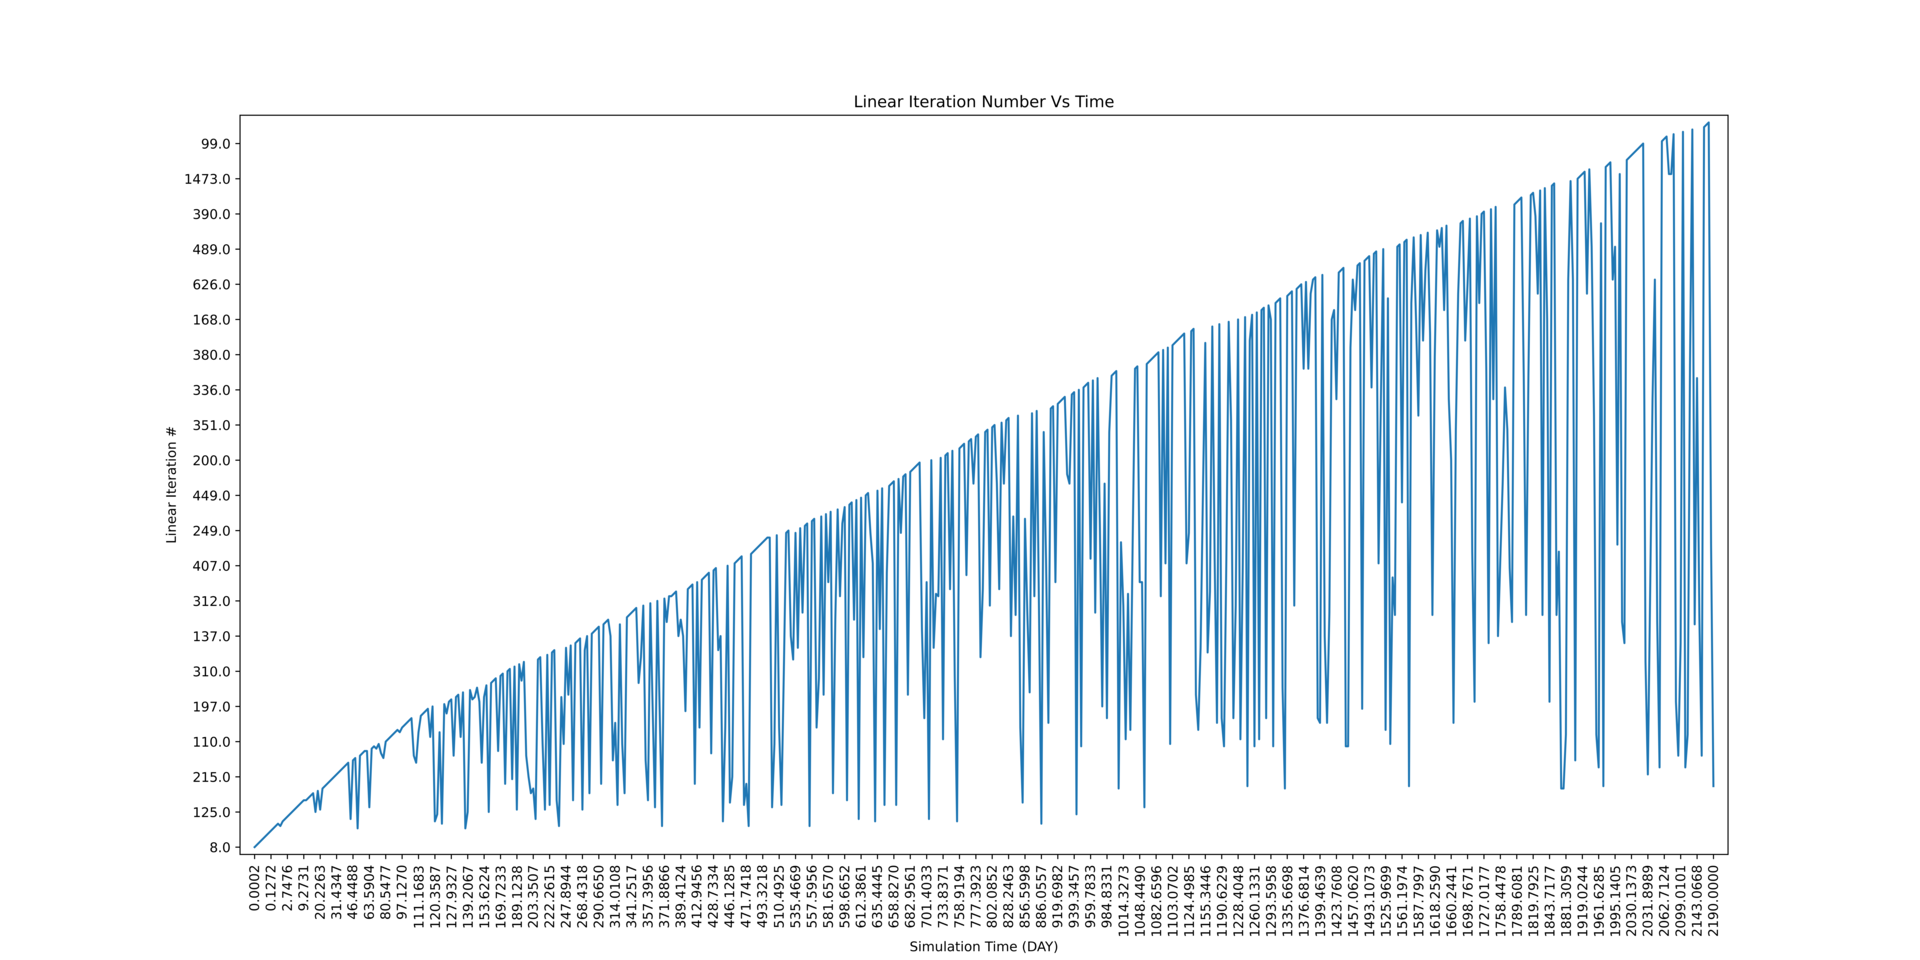
\includegraphics[width=1.1\linewidth]{figures/case2/ilu/its_time.png_reduced.png}
  \caption{\texttt{GMRES-ILU(0)} preconditioner}
	\label{case2_its_ilu}
\end{subfigure}
\begin{subfigure}{.5\textwidth}
  \centering
  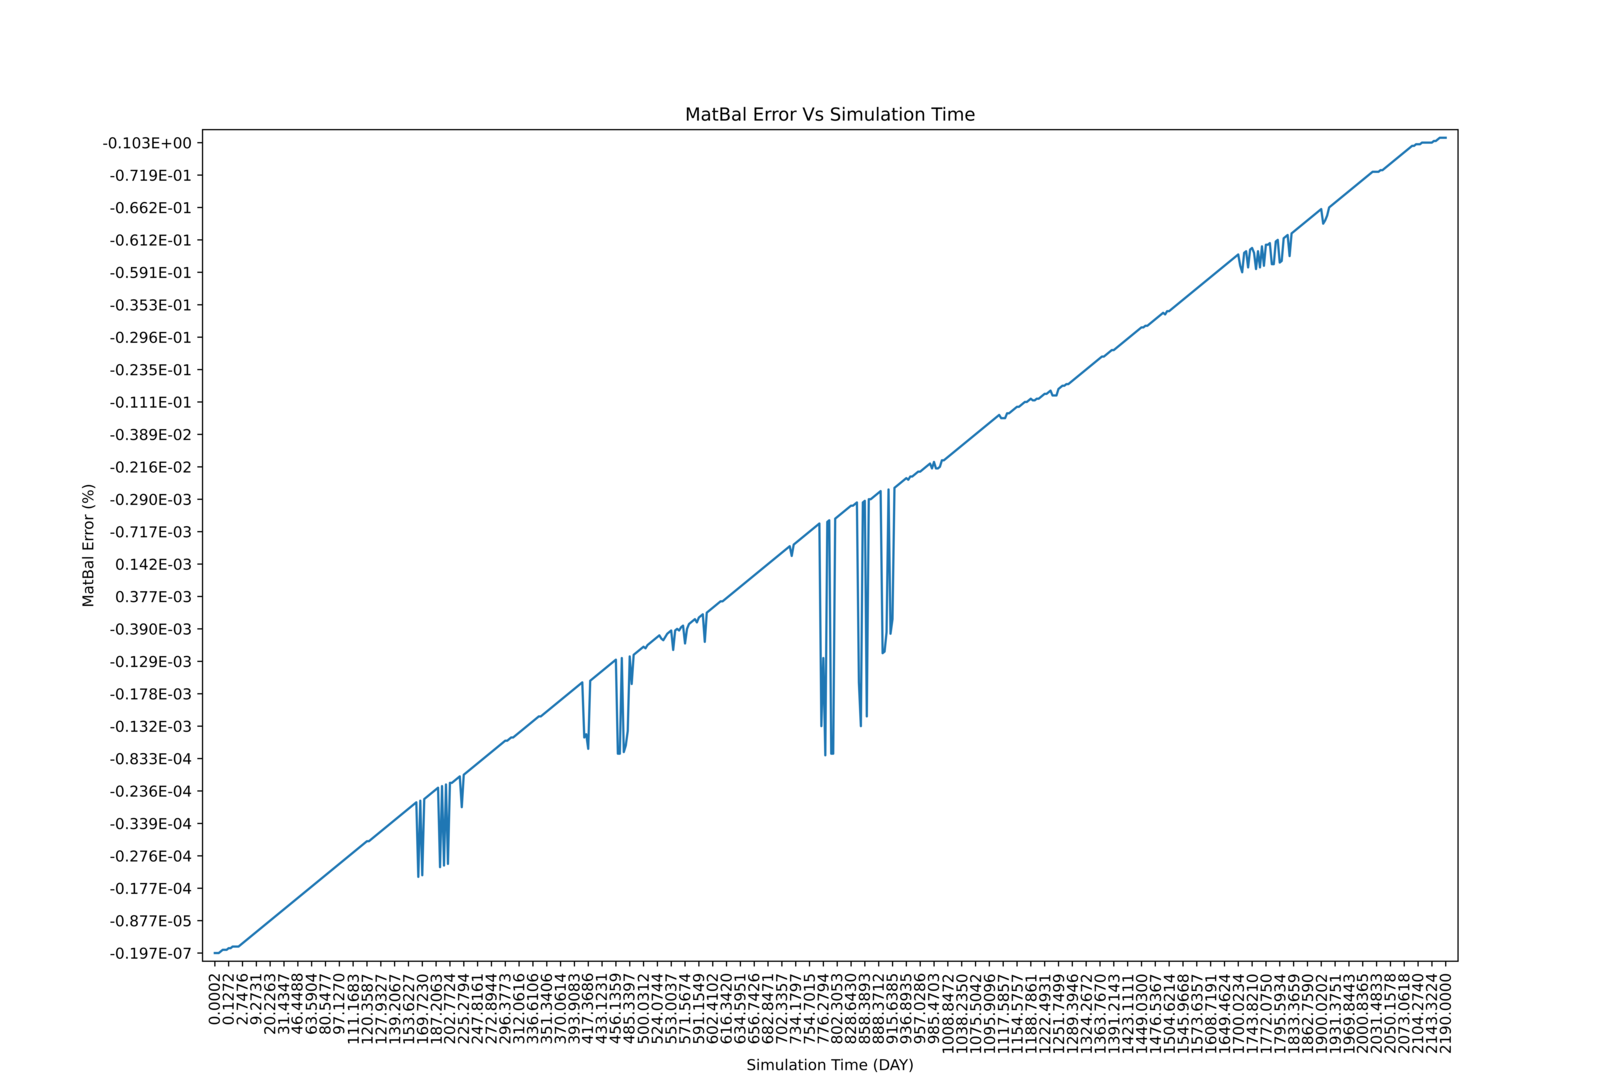
\includegraphics[width=1.1\linewidth]{figures/case2/cpr/matbalerr_time.png_reduced.png}
  \caption{\texttt{CPR-AMG} preconditioner.}
	\label{case2_matbalerr_cpr}
\end{subfigure}%
\begin{subfigure}{.5\textwidth}
  \centering
  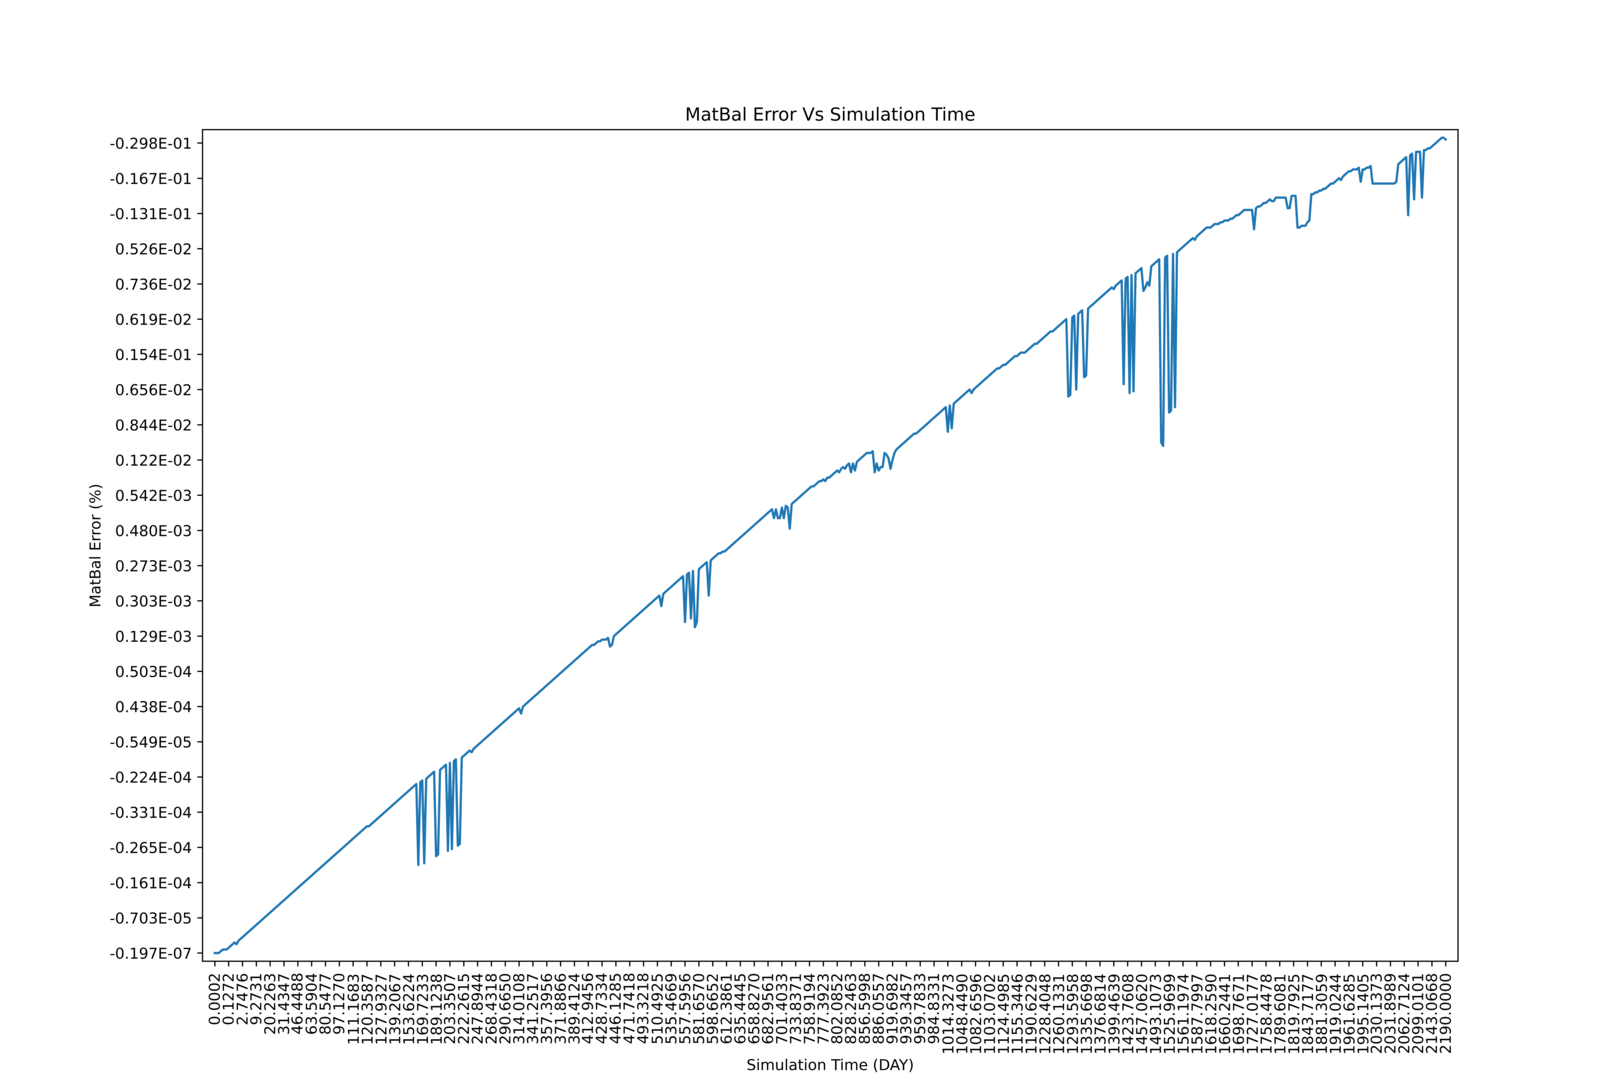
\includegraphics[width=1.1\linewidth]{figures/case2/ilu/matbalerr_time.png_reduced.png}
  \caption{\texttt{GMRES-ILU(0)} preconditioner}
	\label{case2_matbalerr_ilu}
\end{subfigure}
\caption[caption]{A comparison for \texttt{Case 2} for the two different preconditioning methods.\\\hspace{\textwidth}
		\cref{case2_cpu_cpr,case2_cpu_ilu}: CPU run time against simulation time. \\\hspace{\textwidth}
		\cref{case2_its_cpr,case2_its_ilu}: Linear iterations against simulation time.\\\hspace{\textwidth}
		\cref{case2_matbalerr_cpr,case2_matbalerr_ilu}: Material balance error against simulation time.}
\label{case2_param}
\end{figure}
\clearpage

\section{Case 3}

\FloatBarrier
\begin{center}
\begin{table}[h!]
\begin{adjustbox}{width=\textwidth}
    \begin{threeparttable}
    \caption{\textbf{Case 3 Reservoir Parameters\supercite{fernandes}.}}
    \label{case3}
        \begin{tabular}{l r }
            \toprule
            Simulatoin Parameters & Value\\
            \midrule
	\rowcolor{red!20}\textit{\textbf{Reservoir data}}      & \\
	Grid:      &           $200\times200\times10$ ($99,816$ active) \\
	\rowcolor{blue!5}Number of wells:      &  2 (1 injector / 1 producer) \\
	Length, width and thickness:      & $152.4$ m, $304.8$ m and $6.096$ m\\
	\rowcolor{blue!5}Porosity:       &          $0.25$ \\
	Initial water saturation:    & $0.35$ \\      
	\rowcolor{blue!5}Initial pressure:    &      $7.58$ MPa\\
	Formation temperature:    & $313.71$ K     \\
	injector's bottom hole pressure:    &       $8.62$ MPa \\
	\rowcolor{blue!5}Producer’s bottom hole pressure:    &       $7.58$ MPa\\
	Reservoir’s initial composition ($CO_{2}$, $C_{1}$, $C_{2-3}$, $C_{4-6}$, $C_{7-15}$, $C_{16-27}$, $C_{28+}$) & $0.0337$, $0.0861$, $0.1503$, $0.1671$, $0.3304$, $0.1611$ and $0.0713$\\
	\rowcolor{blue!5}Injection fluid composition ($CO_{2}$, $C_{1}$):    &   $0.95$, $0.05$\\
        \bottomrule
        \end{tabular}
    \end{threeparttable}
\end{adjustbox}    
\end{table}
\end{center}
\FloatBarrier

\begin{table}[h!]
   \caption{Comparison parameters for \texttt{Case 3}.}
   \label{case3-tab}
   \small
   \centering
   \begin{tabular}{lcc}
   \toprule\toprule
   \textbf{Variable} & \textbf{CPR-AMG} & \textbf{GMRES-ILU(0)} \\
   \midrule
   CPU Time (hr) & 4.58 & 6.71 \\
   Solver Time (hr) & 1.7 & 3.89 \\
   \# Newton Iterations & 1,463 & 1,438 \\
   \# Solver Iterations & 5,152 & 24,068\\
   \# Time Steps & 451 & 454 \\
   \bottomrule
   \end{tabular}
\end{table}

\begin{figure}
\centering
\begin{subfigure}{.5\textwidth}
  \centering
  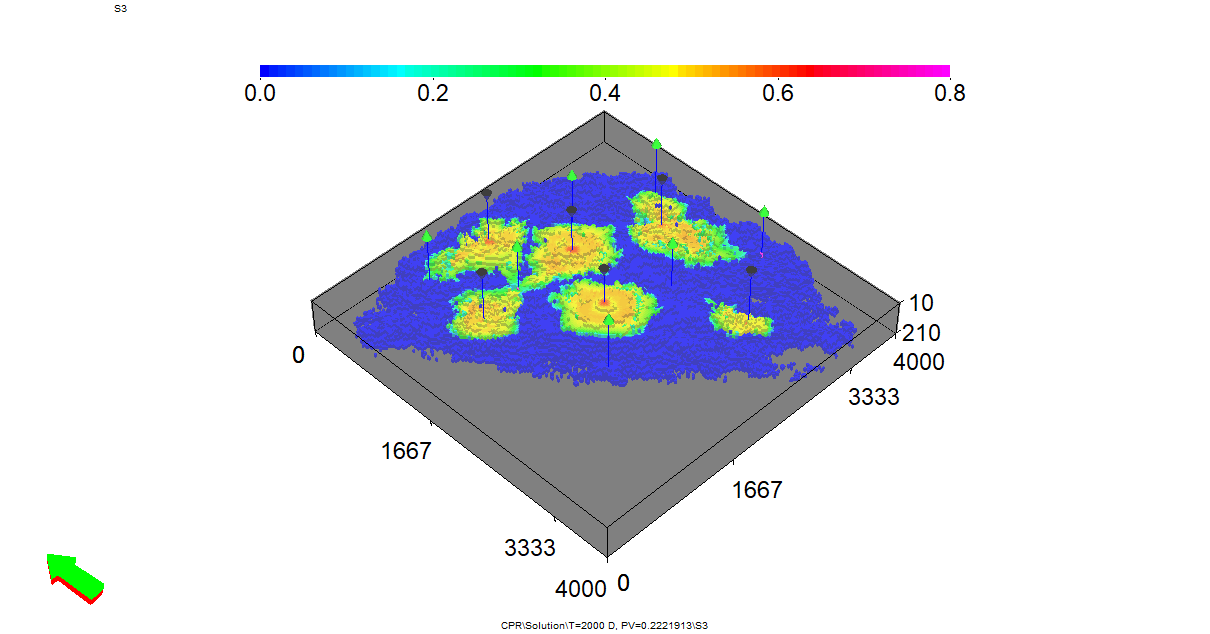
\includegraphics[width=1.3\linewidth]{figures/case3_cpr_sgas.png}
  \caption{\texttt{CPR-AMG} preconditioner.}
\end{subfigure}%
\begin{subfigure}{.5\textwidth}
  \centering
  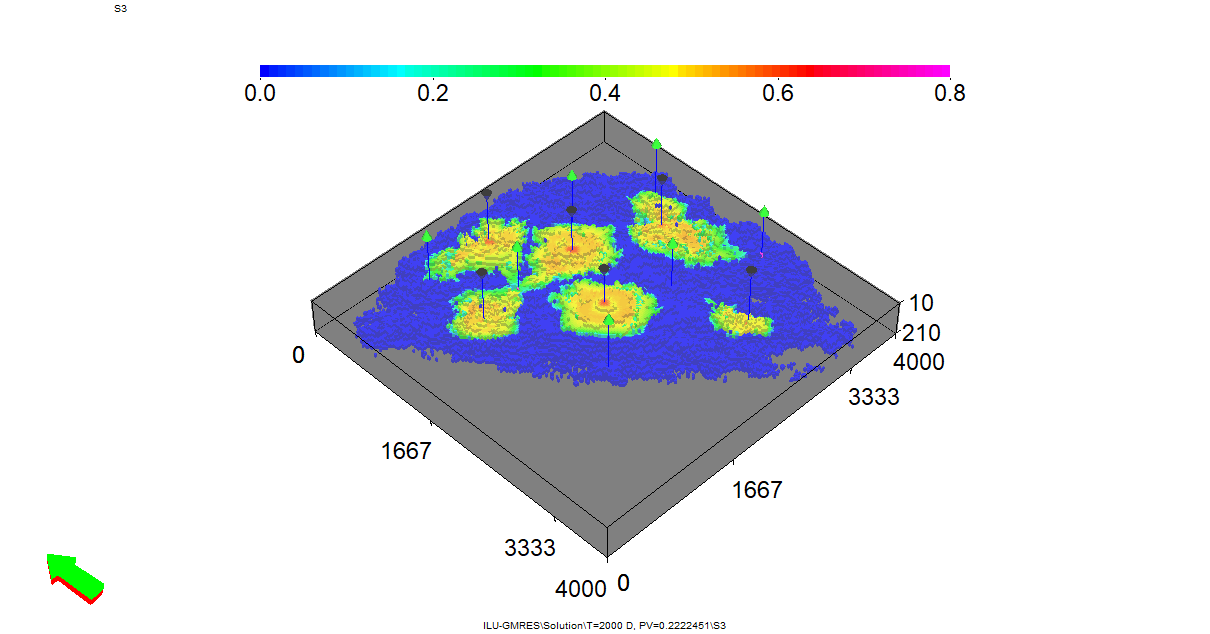
\includegraphics[width=1.3\linewidth]{figures/case3_ilu_sgas.png}
  \caption{\texttt{GMRES-ILU(0)} preconditioner}
\end{subfigure}
\caption{A comparison of \texttt{Case 3} gas saturation $S_{g}$ distribution for the two different preconditioning methods after 2000 days of simulation.}
\label{case3sg}
\end{figure}

\begin{figure}
\centering
\begin{subfigure}{.5\textwidth}
  \centering
  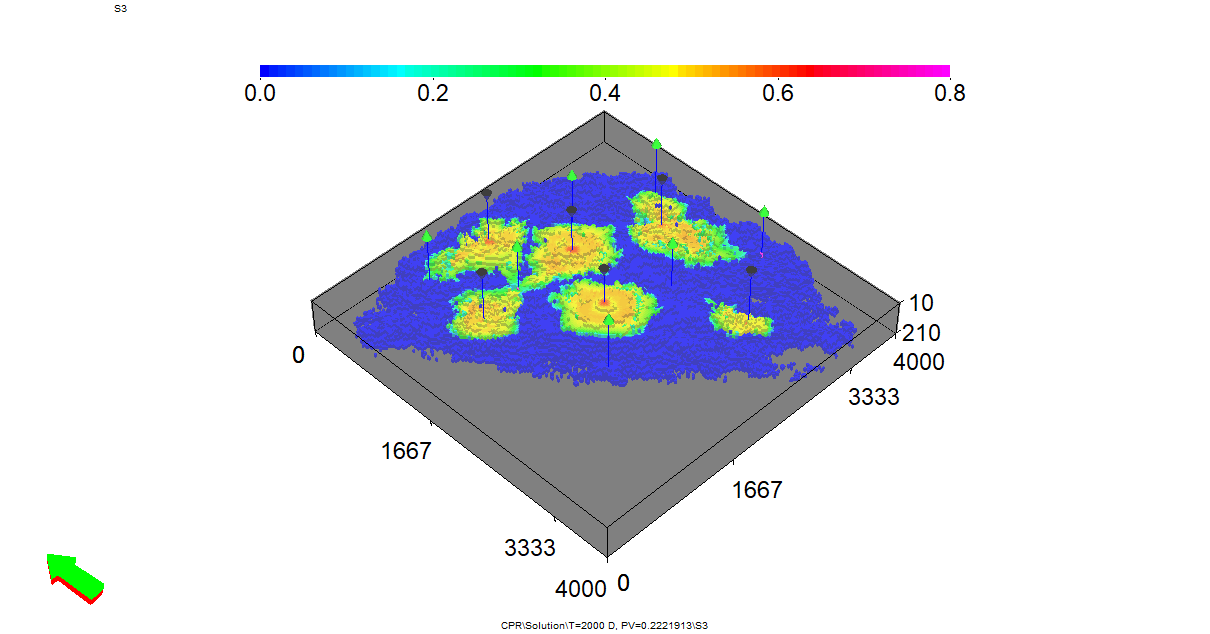
\includegraphics[width=1.3\linewidth]{figures/case3_cpr_sgas.png}
  \caption{\texttt{CPR-AMG} preconditioner.}
\end{subfigure}%
\begin{subfigure}{.5\textwidth}
  \centering
  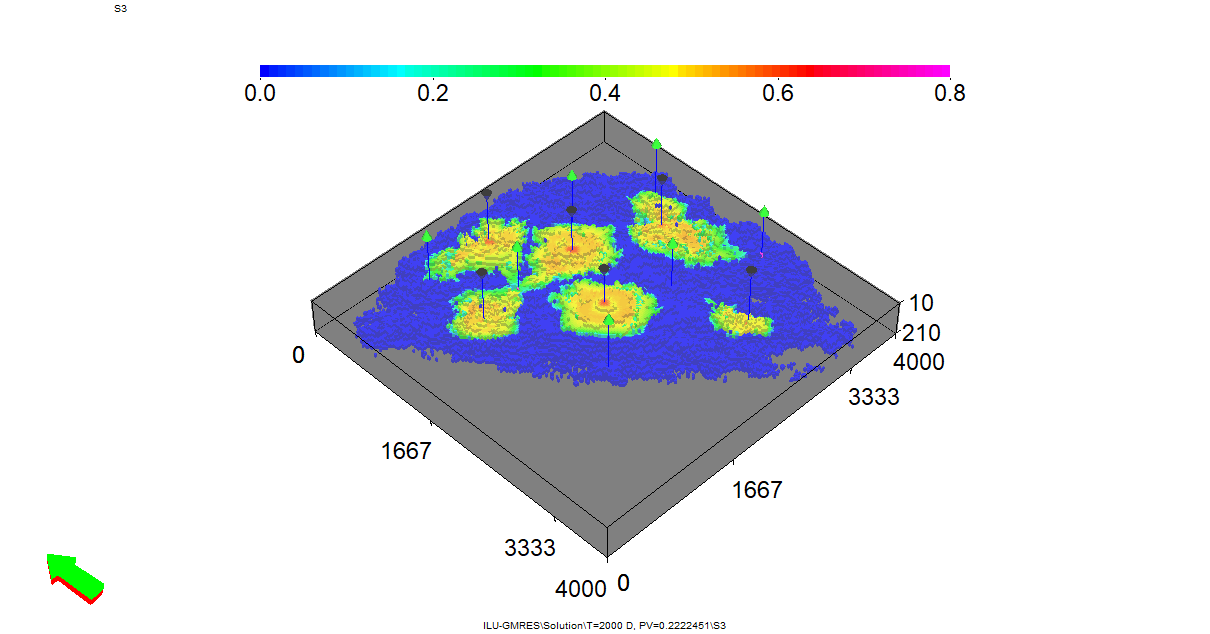
\includegraphics[width=1.3\linewidth]{figures/case3_ilu_sgas.png}
  \caption{\texttt{GMRES-ILU(0)} preconditioner}
\end{subfigure}
\caption{A comparison of \texttt{Case 3} $CO_{2}$ overall composition $Z_{CO_{2}}$ distribution for the two different preconditioning methods after 2000 days of simulation.}
\label{case3z}
\end{figure}

\begin{figure}
\centering
\begin{subfigure}{.5\textwidth}
  \centering
  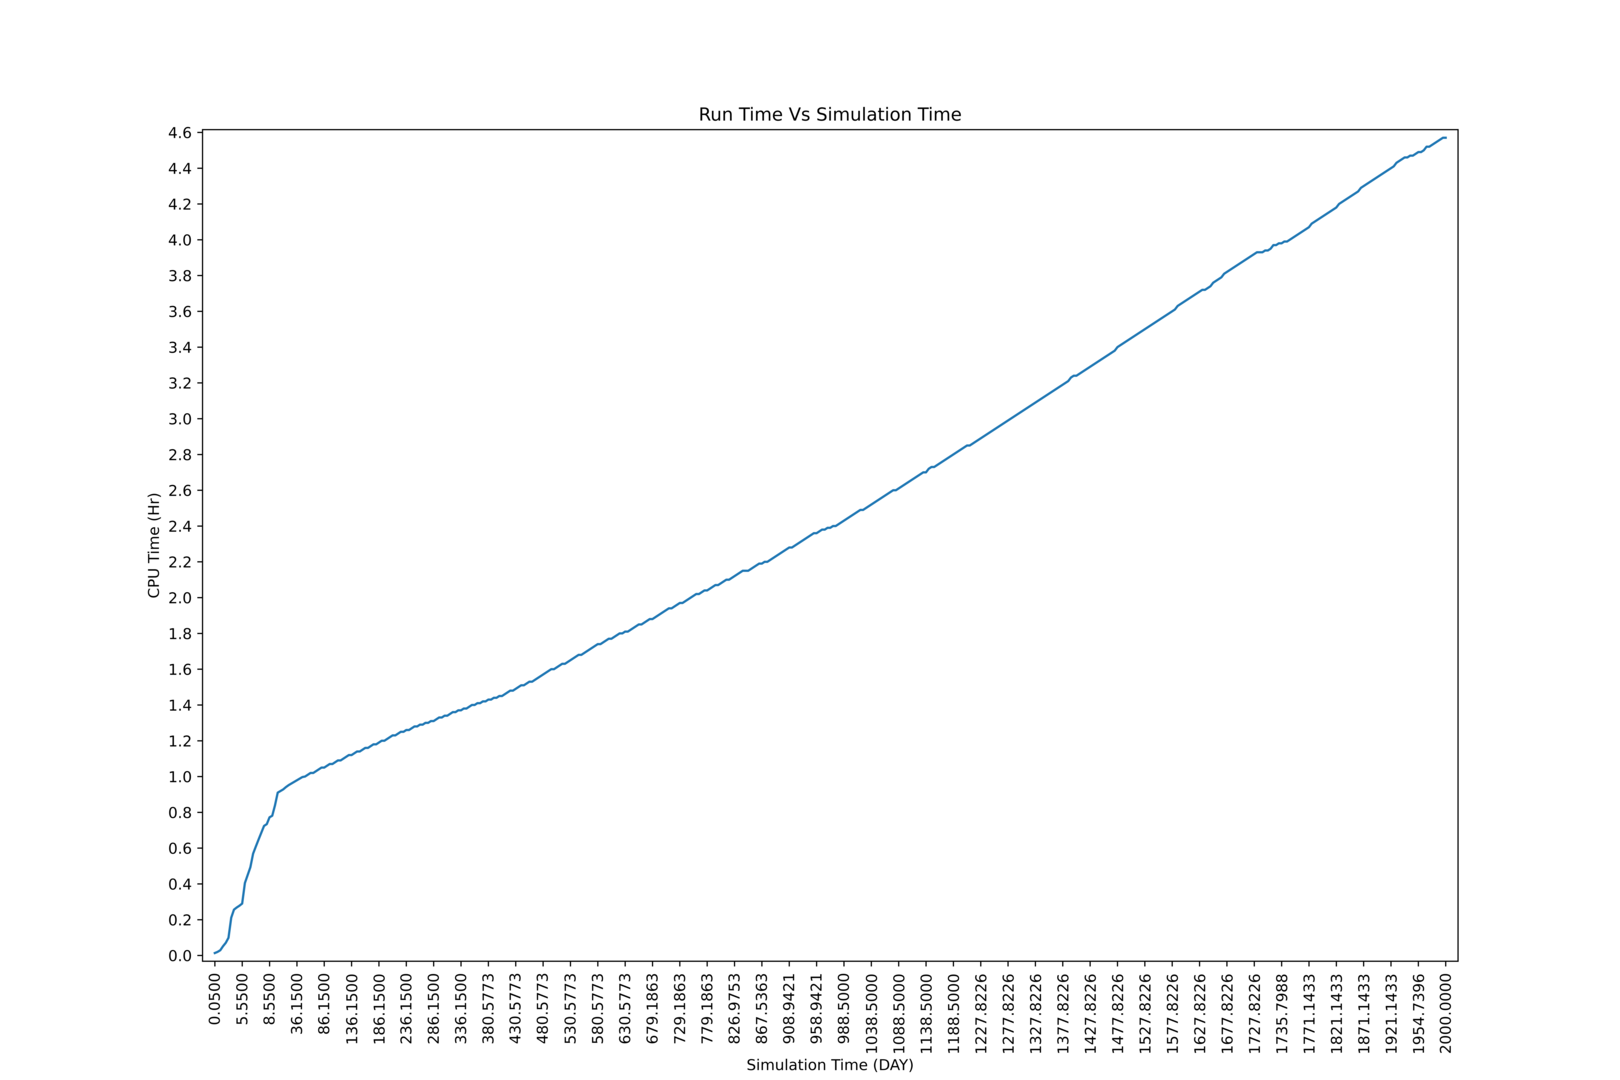
\includegraphics[width=1.1\linewidth]{figures/case3/cpr/cpu_time.png_reduced.png}
  \caption{\texttt{CPR-AMG} preconditioner.}
	\label{case3_cpu_cpr}
\end{subfigure}%
\begin{subfigure}{.5\textwidth}
  \centering
  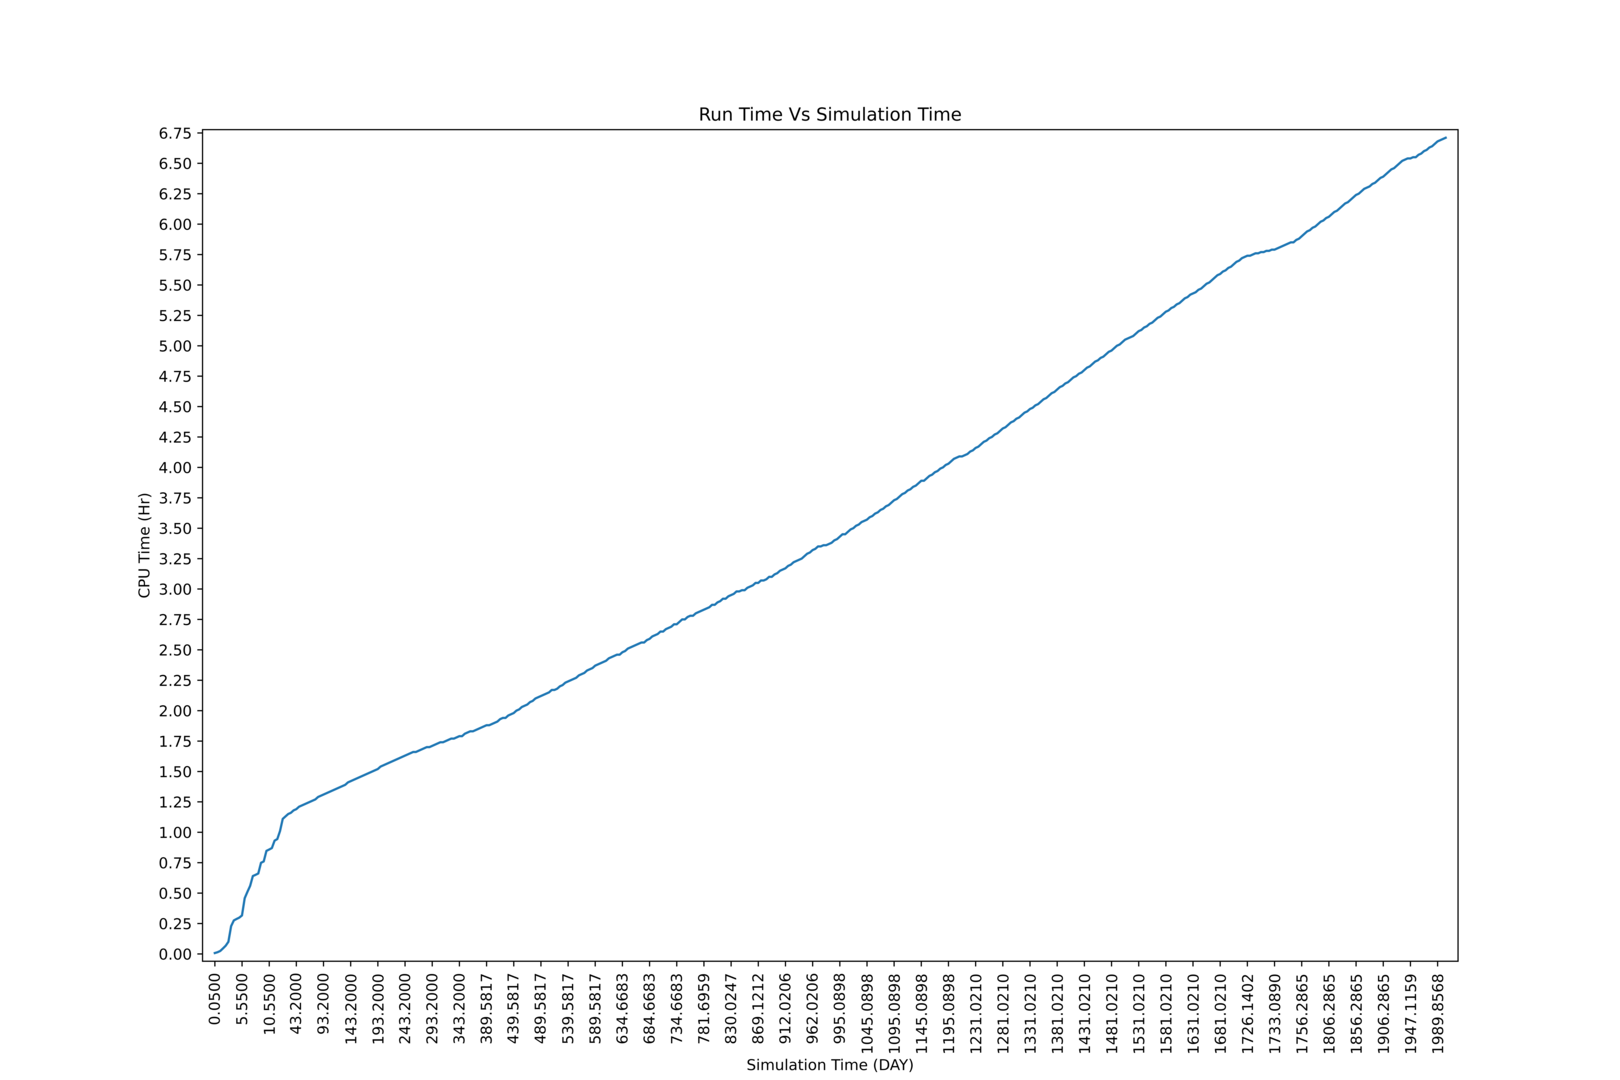
\includegraphics[width=1.1\linewidth]{figures/case3/ilu/cpu_time.png_reduced.png}
  \caption{\texttt{GMRES-ILU(0)} preconditioner}
	\label{case3_cpu_ilu}
\end{subfigure}
\begin{subfigure}{.5\textwidth}
  \centering
  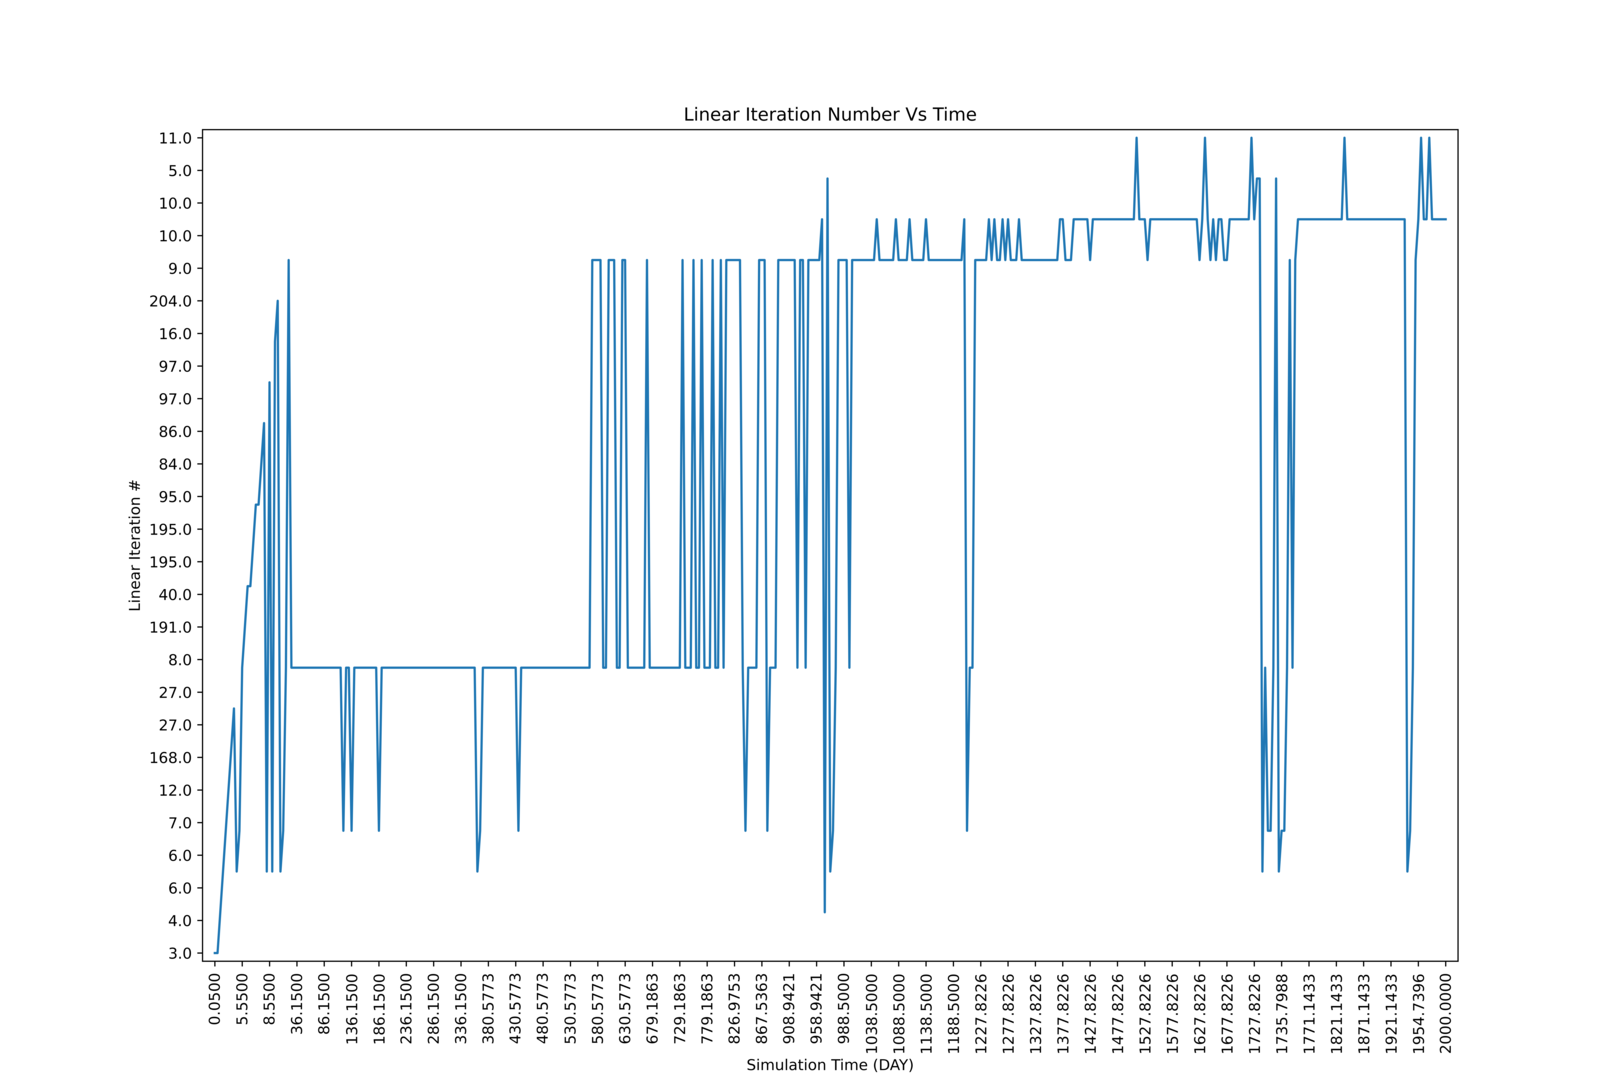
\includegraphics[width=1.1\linewidth]{figures/case3/cpr/its_time.png_reduced.png}
  \caption{\texttt{CPR-AMG} preconditioner.}
	\label{case3_its_cpr}
\end{subfigure}%
\begin{subfigure}{.5\textwidth}
  \centering
  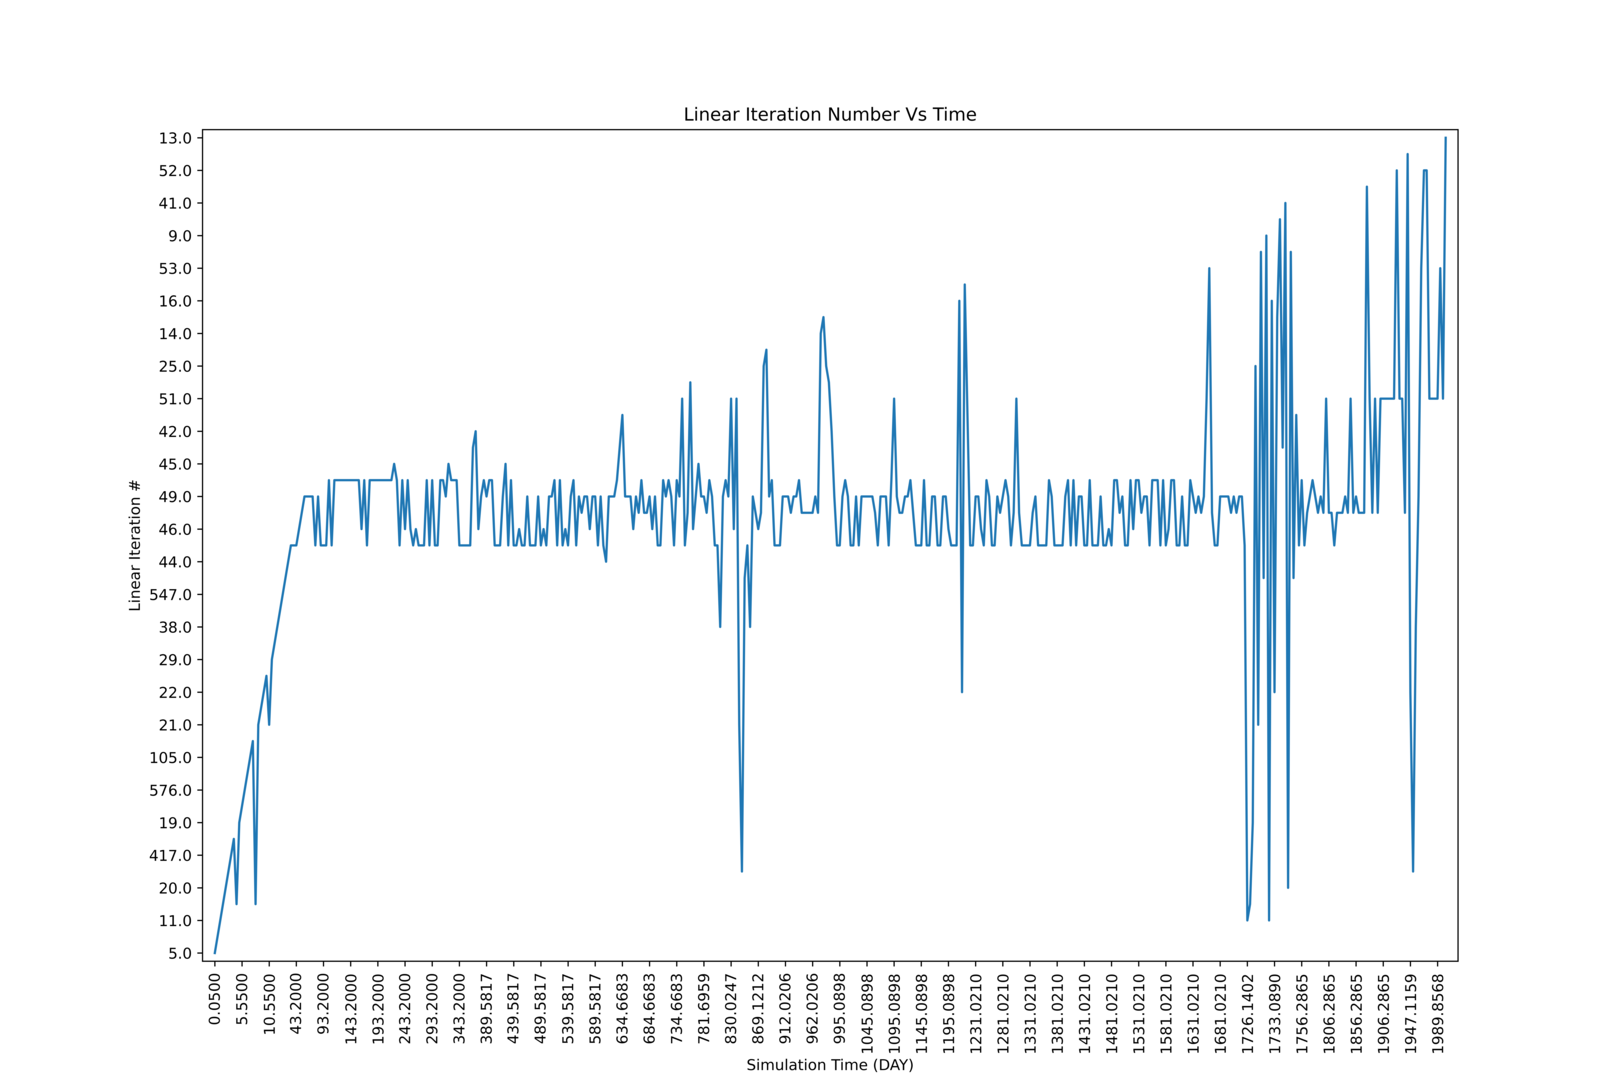
\includegraphics[width=1.1\linewidth]{figures/case3/ilu/its_time.png_reduced.png}
  \caption{\texttt{GMRES-ILU(0)} preconditioner}
	\label{case3_its_ilu}
\end{subfigure}
\begin{subfigure}{.5\textwidth}
  \centering
  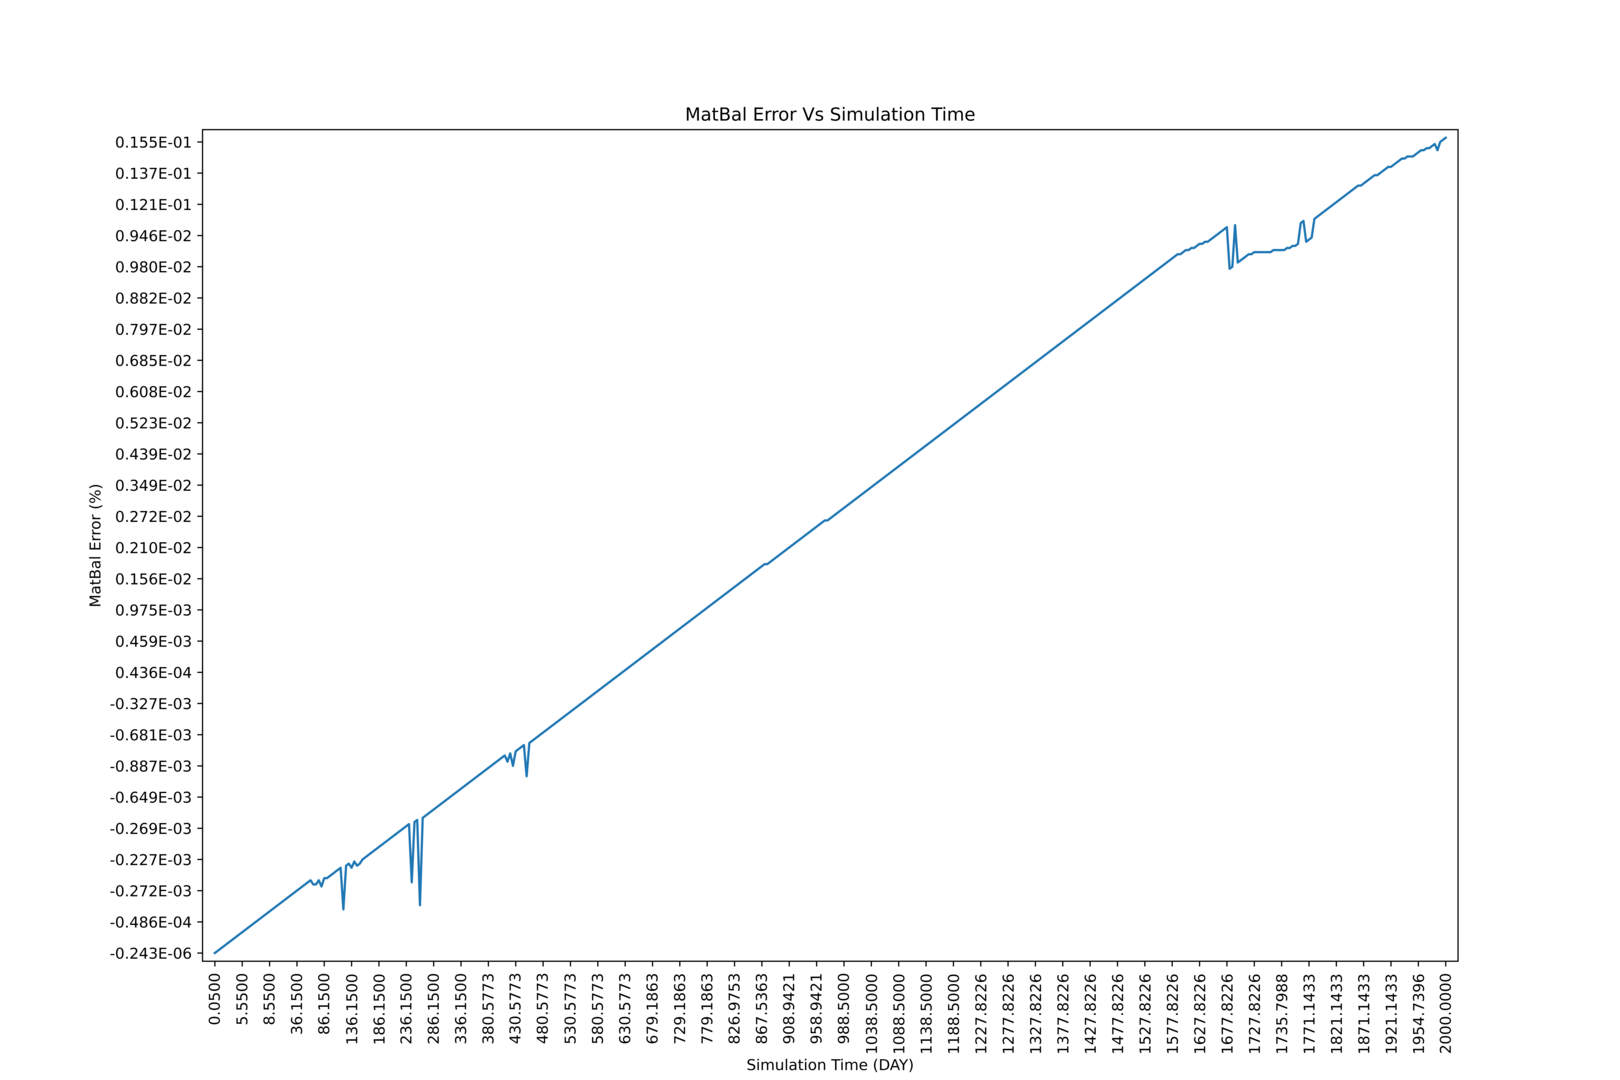
\includegraphics[width=1.1\linewidth]{figures/case3/cpr/matbalerr_time.png_reduced.png}
  \caption{\texttt{CPR-AMG} preconditioner.}
	\label{case3_matbalerr_cpr}
\end{subfigure}%
\begin{subfigure}{.5\textwidth}
  \centering
  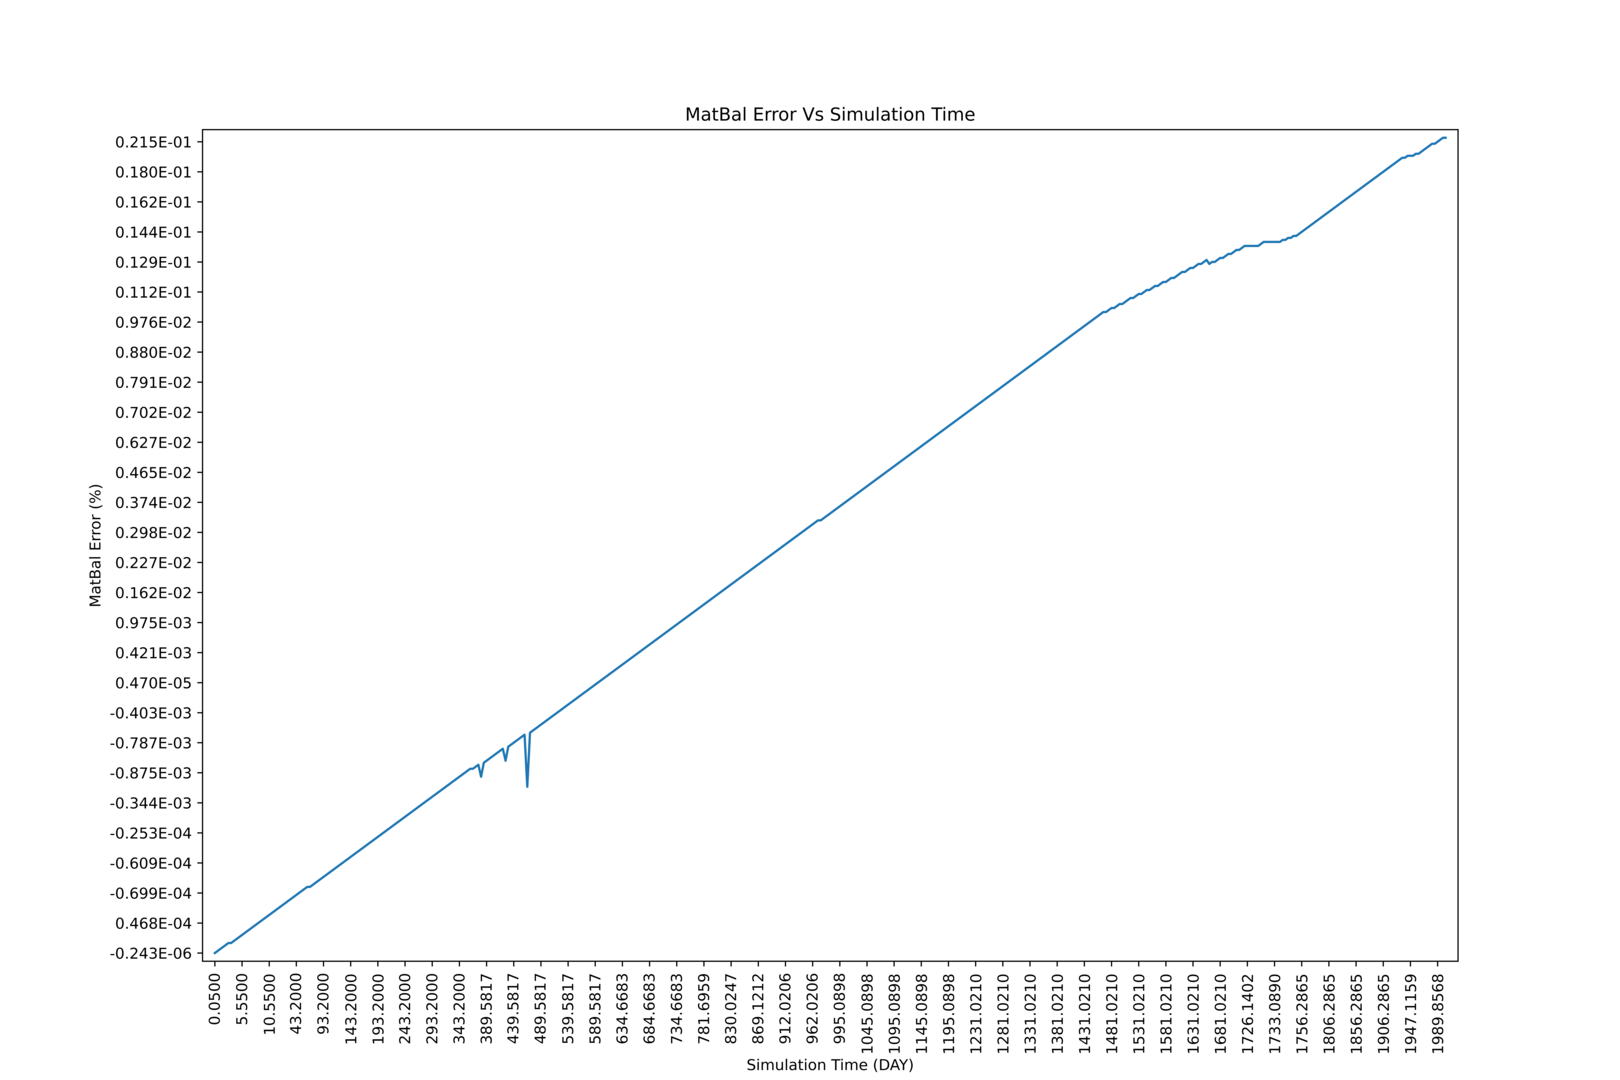
\includegraphics[width=1.1\linewidth]{figures/case3/ilu/matbalerr_time.png_reduced.png}
  \caption{\texttt{GMRES-ILU(0)} preconditioner}
	\label{case3_matbalerr_ilu}
\end{subfigure}
\caption[caption]{A comparison for \texttt{Case 3} for the two different preconditioning methods.\\\hspace{\textwidth}
		\cref{case3_cpu_cpr,case3_cpu_ilu}: CPU run time against simulation time. \\\hspace{\textwidth}
		\cref{case3_its_cpr,case3_its_ilu}: Linear iterations against simulation time.\\\hspace{\textwidth}
		\cref{case3_matbalerr_cpr,case3_matbalerr_ilu}: Material balance error against simulation time.}
\label{case3sg}
\end{figure}
\clearpage

\section{Case 4}
This model simulates water flooding in a fractured reservoir. All wells are controlled by fixing bottomhole pressure.
\FloatBarrier
\begin{center}
\begin{table}[h!]
\begin{adjustbox}{width=0.7\textwidth}
    \begin{threeparttable}
    \caption{\textbf{Case 4 Reservoir Parameters\supercite{phdfernandes}.}}
    \label{case4}
        \begin{tabular}{l r }
            \toprule
            Simulatoin Parameters & Value\\
            \midrule
	\rowcolor{red!20}\textit{\textbf{Reservoir data}}      & \\
	Grid:      &           $200\times400\times25$ ($465,816$ active) \\
	\rowcolor{blue!5}Number of wells:      &  49 (25 injector / 24 producer) \\
	Length, width and thickness:      & $4,000$ ft, $8,000$ ft and $150$ ft\\
	\rowcolor{blue!5}Porosity:       &          $0.30$ \\
	Permeability ($X, \ Y, \ Z$) & $10, \ 10$ and $1$ mD\\
	\rowcolor{blue!5}Fracture permeability & $10,000$ mD\\
	Fracture aperture	& $0.01$ ft\\
	\rowcolor{blue!5}Initial water saturation:    & $0.17$ \\      
	Formation temperature:    & $86$ F$^{\circ}$     \\
	\rowcolor{blue!5}Initial pressure:    &      $3,000$ psi\\
	Reservoir’s initial composition ($C_{1}$, $C_{3}$, $C_{10}$) & $0.01$, $0.19$, $0.8$\\
        \bottomrule
        \end{tabular}
    \end{threeparttable}
\end{adjustbox}    
\end{table}
\end{center}
\FloatBarrier

\begin{table}[h!]
   \caption{Comparison parameters for \texttt{Case 4}.}
   \label{case4-tab}
   \small
   \centering
   \begin{tabular}{lcc}
   \toprule\toprule
   \textbf{Variable} & \textbf{CPR-AMG} & \textbf{GMRES-ILU(0)} \\
   \midrule
   CPU Time (hr) & 14.4 & 25.6 \\
   Solver Time (hr) & 10.3 & 21.7 \\
   \# Newton Iterations & 3,164 & 3,169 \\
   \# Solver Iterations & 9,572 & 88,872 \\
   \# Time Steps & 849 & 850 \\
   \bottomrule
   \end{tabular}
\end{table}

\begin{figure}
\centering
\begin{subfigure}{.5\textwidth}
  \centering
  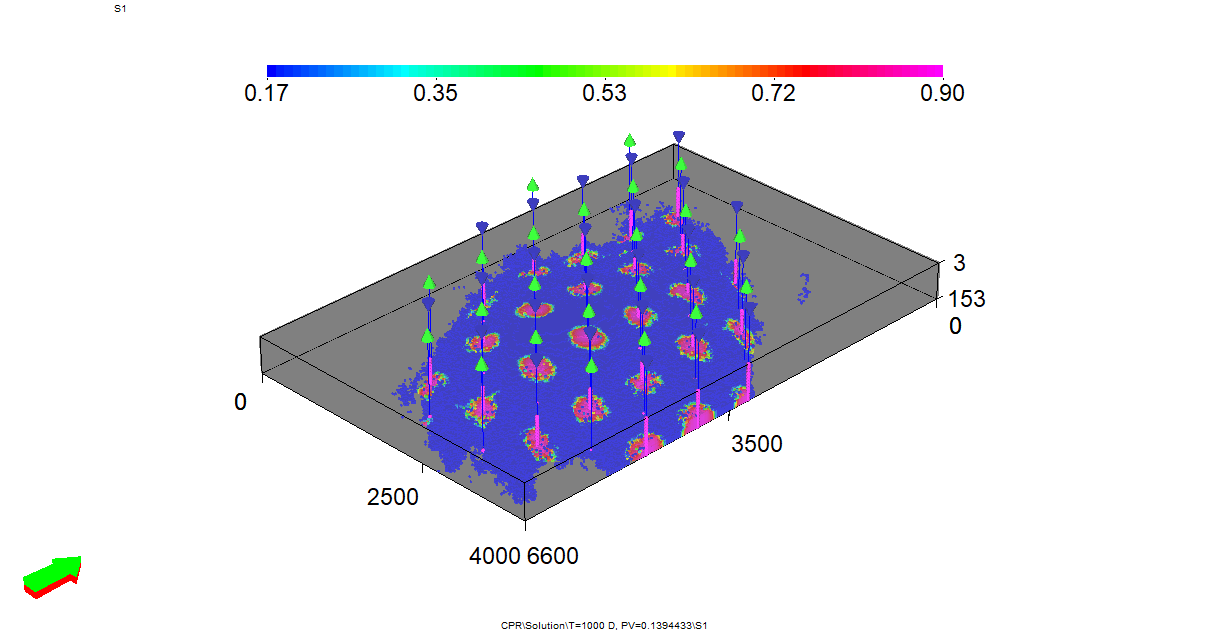
\includegraphics[width=1.3\linewidth]{figures/Case8_CPR_Sw.png}
  \caption{\texttt{CPR-AMG} preconditioner.}
\end{subfigure}%
\begin{subfigure}{.5\textwidth}
  \centering
  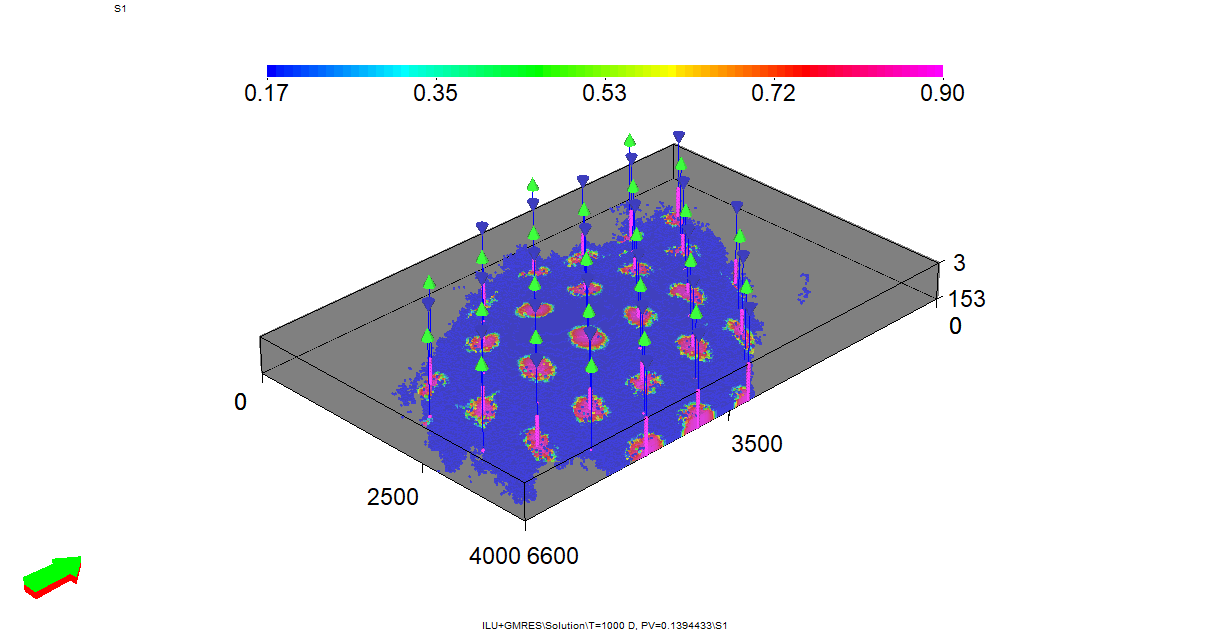
\includegraphics[width=1.3\linewidth]{figures/Case8_ILU-GMRES_Sw.png}
  \caption{\texttt{GMRES-ILU(0)} preconditioner}
\end{subfigure}
\caption{A comparison of \texttt{Case 4} water saturation $S_{w}$ distribution for the two different preconditioning methods after 1000days of simulation.}
\label{case4sw}
\end{figure}

\begin{figure}
\centering
\begin{subfigure}{.5\textwidth}
  \centering
  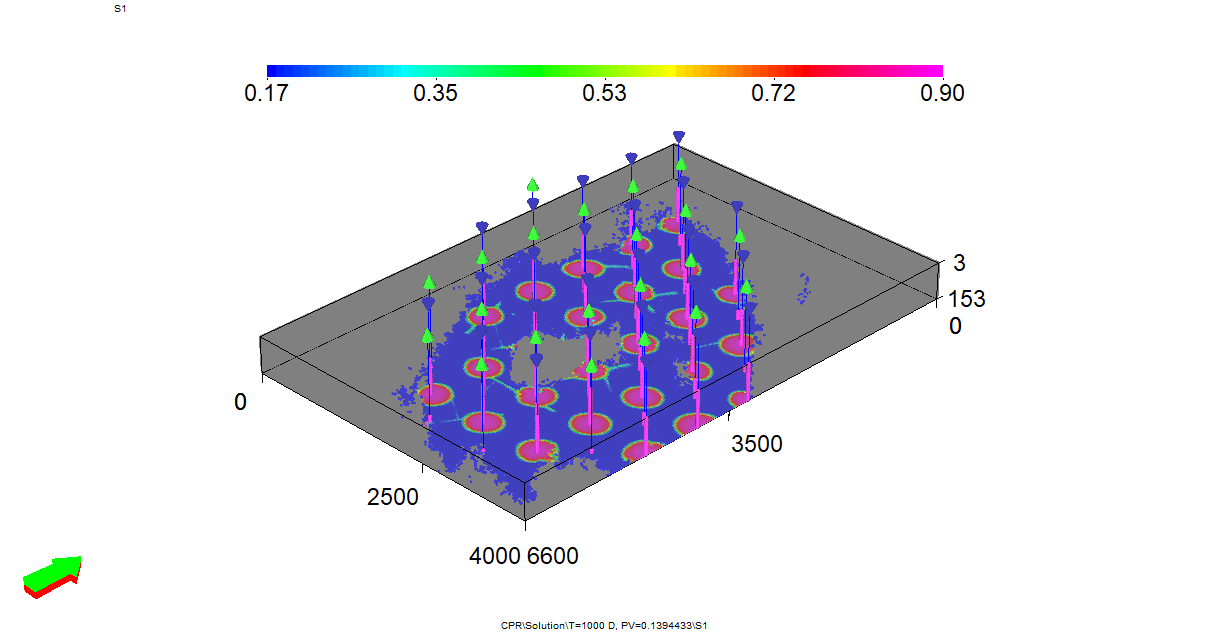
\includegraphics[width=1.3\linewidth]{figures/Case8_CPR_Sw_bl.png}
  \caption{\texttt{CPR-AMG} preconditioner.}
\end{subfigure}%
\begin{subfigure}{.5\textwidth}
  \centering
  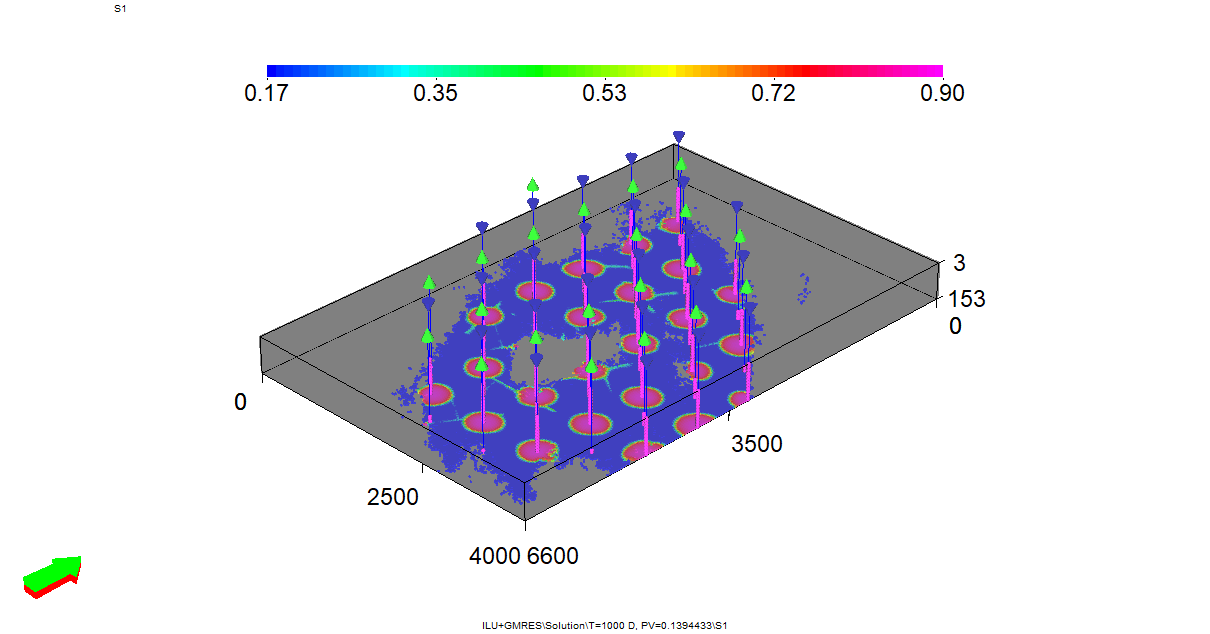
\includegraphics[width=1.3\linewidth]{figures/Case8_ILU-GMRES_Sw_bl.png}
  \caption{\texttt{GMRES-ILU(0)} preconditioner}
\end{subfigure}
\caption{A comparison of \texttt{Case 4} water saturation $S_{w}$ bottom layer for the two different preconditioning methods after 10000 days of simulation.}
\label{case4swbl}
\end{figure}

\begin{figure}
\centering
\begin{subfigure}{.5\textwidth}
  \centering
  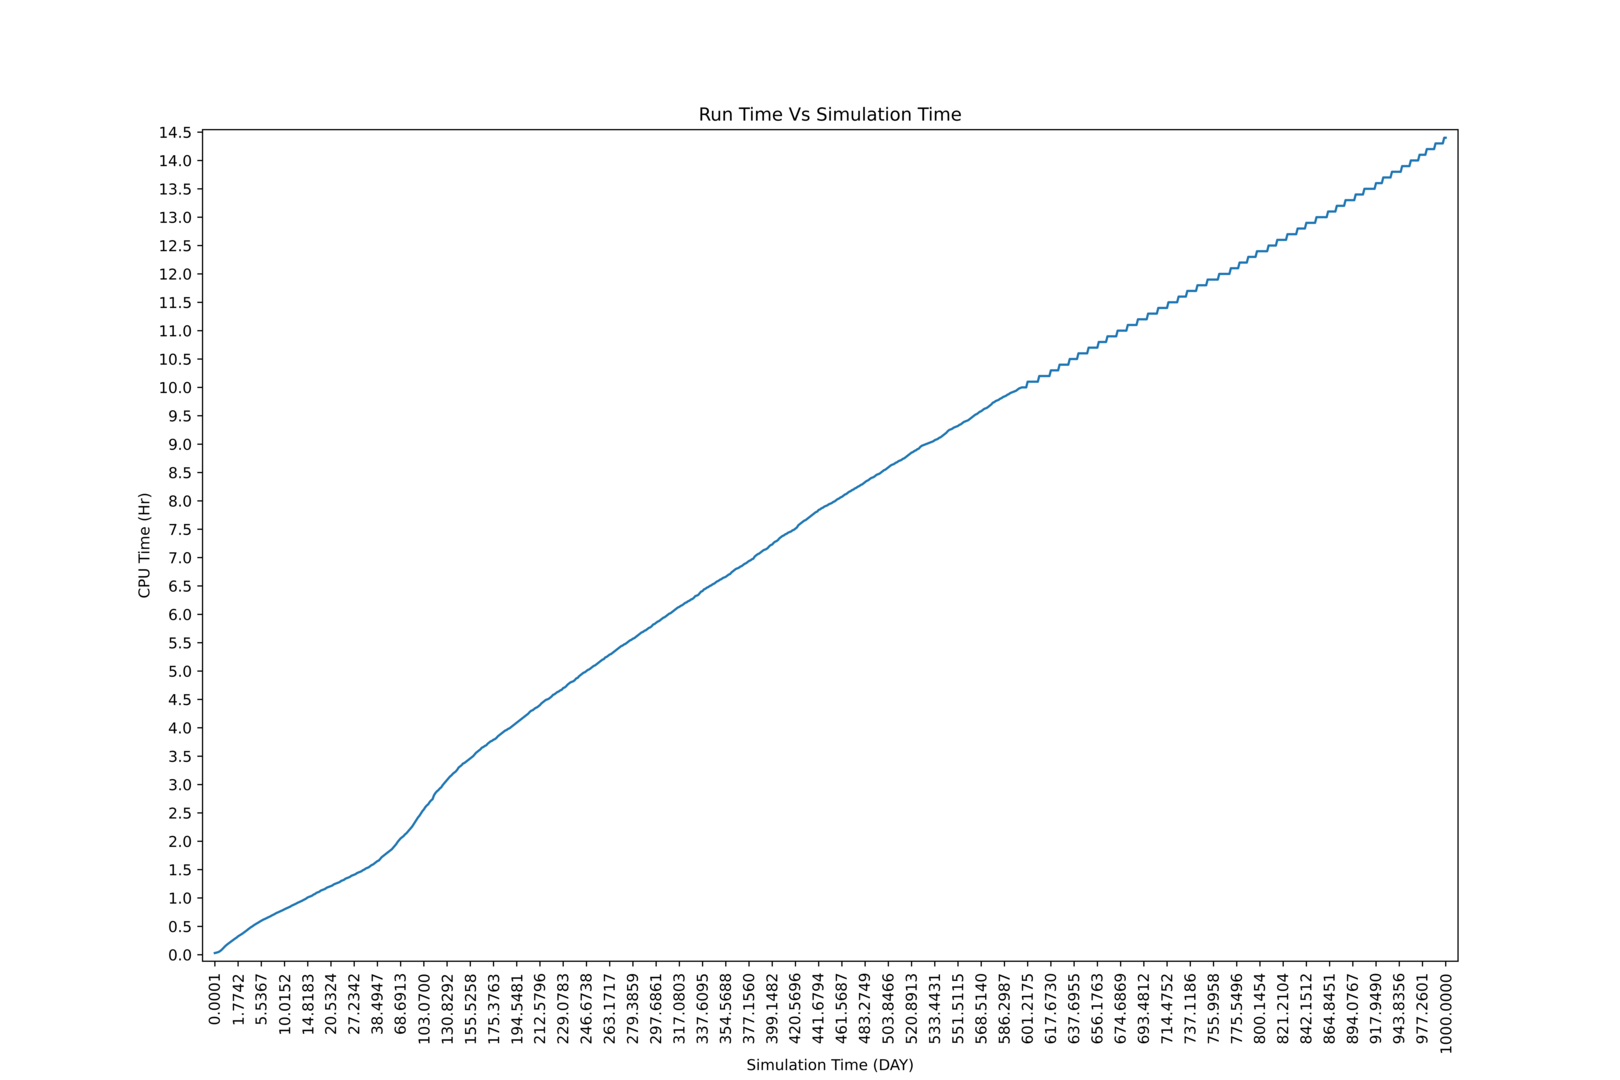
\includegraphics[width=1.1\linewidth]{figures/case8/cpr/cpu_time.png_reduced.png}
  \caption{\texttt{CPR-AMG} preconditioner.}
	\label{case8_cpu_cpr}
\end{subfigure}%
\begin{subfigure}{.5\textwidth}
  \centering
  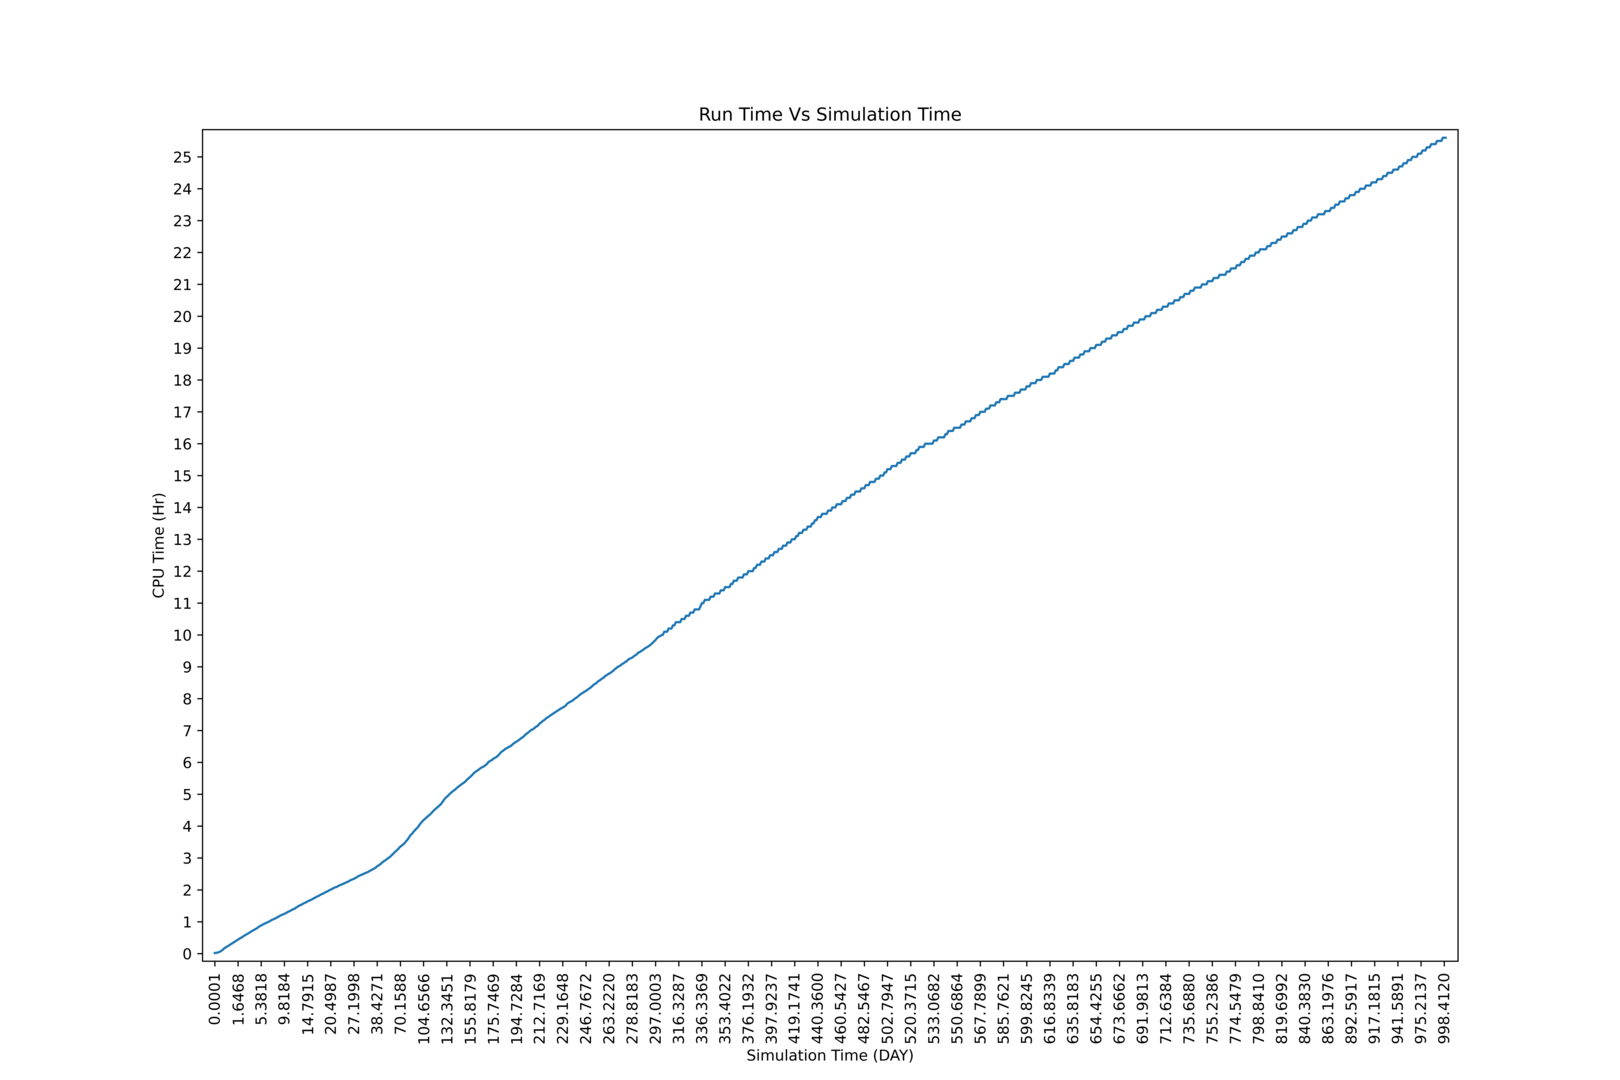
\includegraphics[width=1.1\linewidth]{figures/case8/ilu/cpu_time.png_reduced.png}
  \caption{\texttt{GMRES-ILU(0)} preconditioner}
	\label{case8_cpu_ilu}
\end{subfigure}
\begin{subfigure}{.5\textwidth}
  \centering
  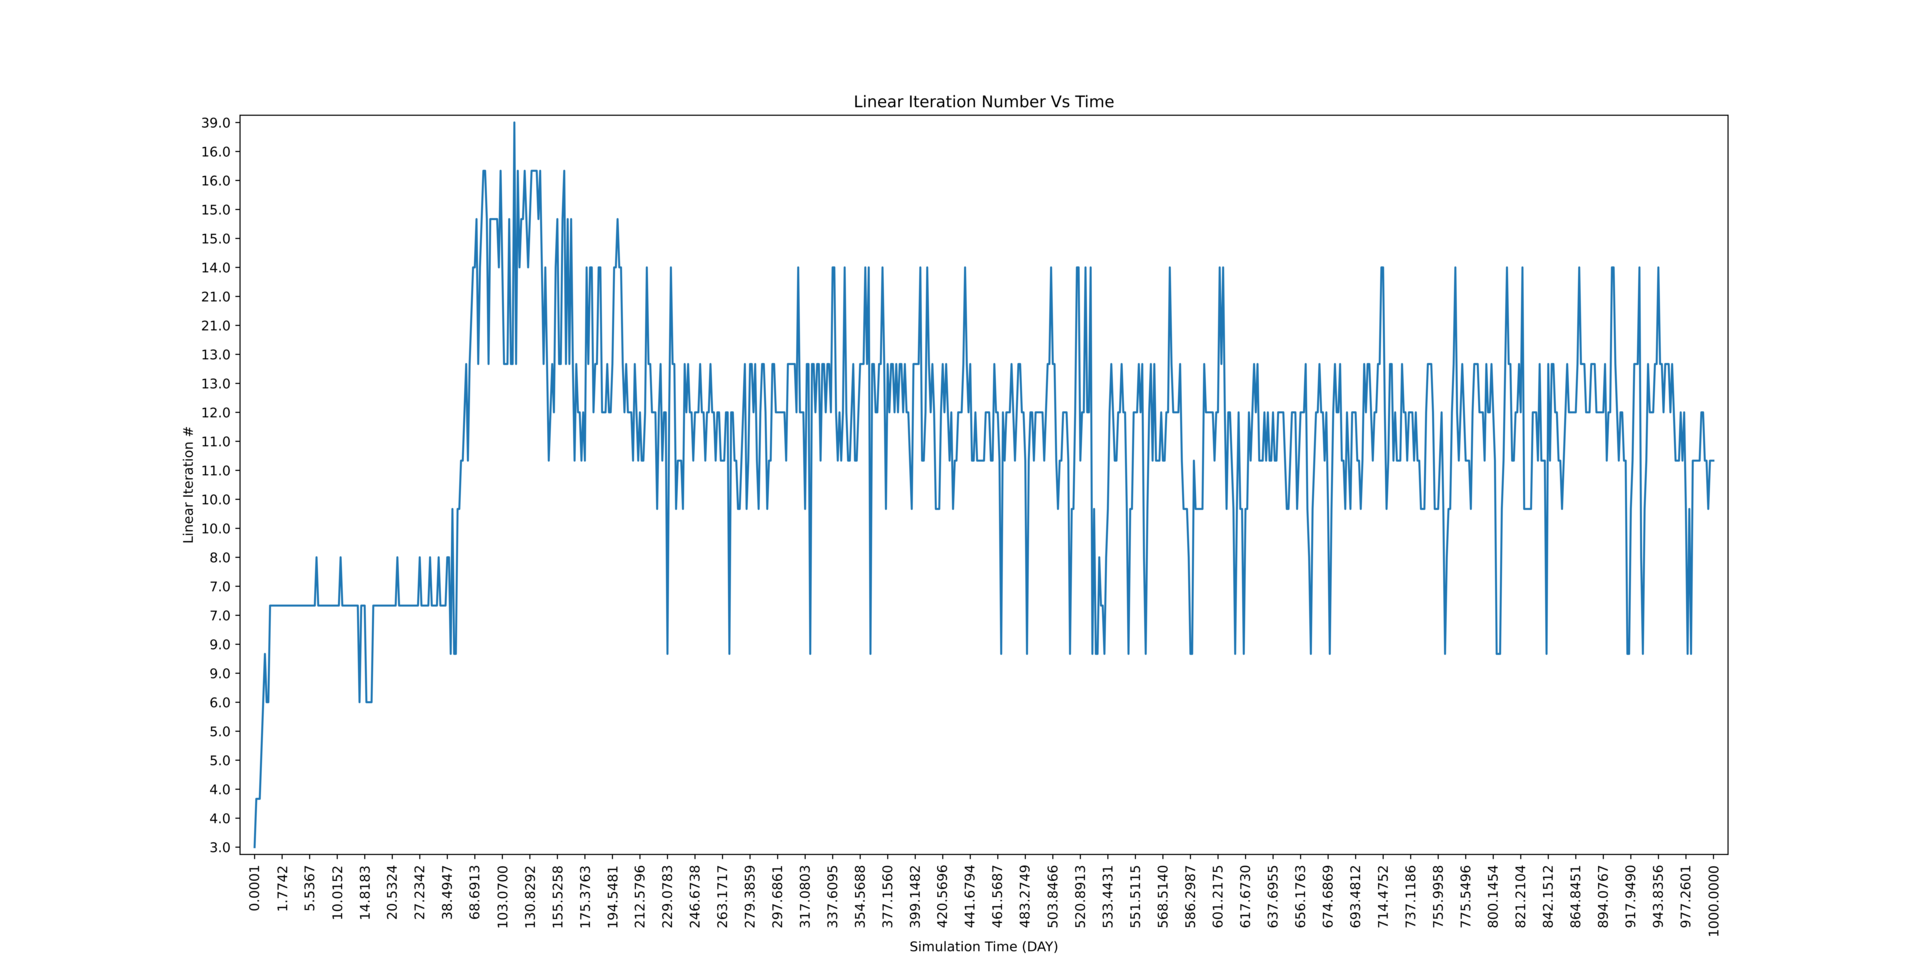
\includegraphics[width=1.1\linewidth]{figures/case8/cpr/its_time.png_reduced.png}
  \caption{\texttt{CPR-AMG} preconditioner.}
	\label{case8_its_cpr}
\end{subfigure}%
\begin{subfigure}{.5\textwidth}
  \centering
  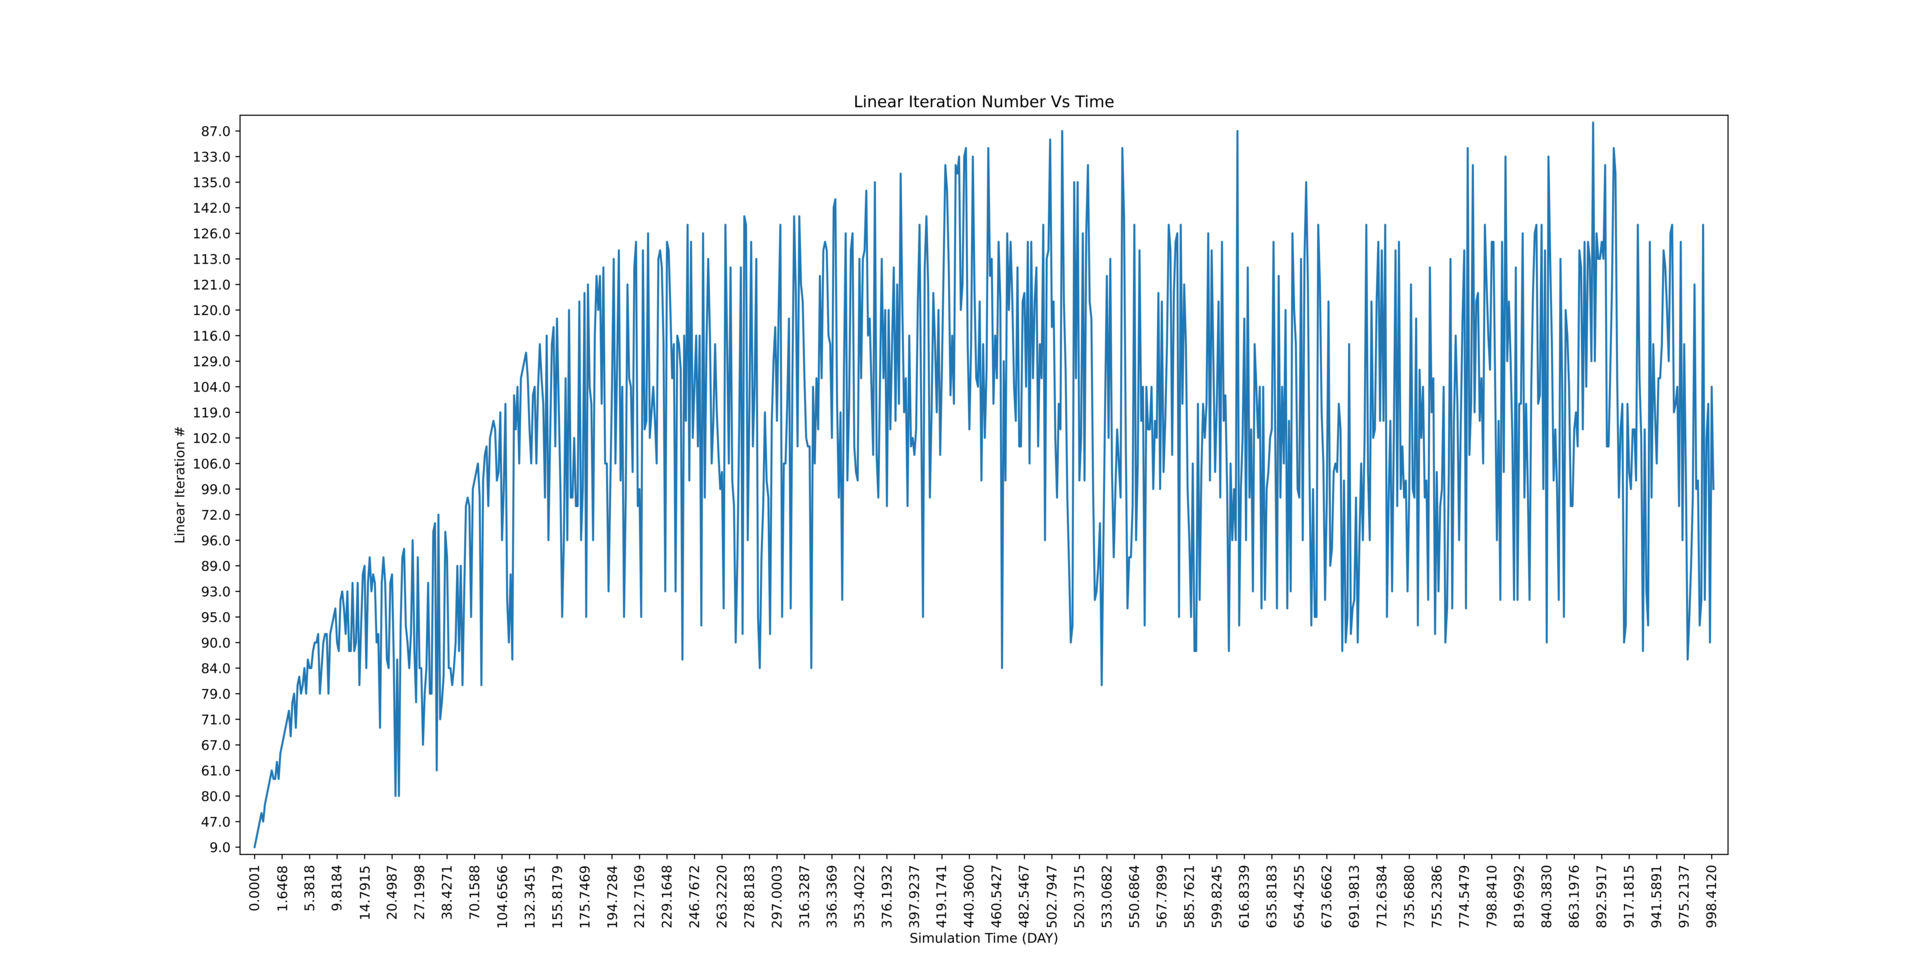
\includegraphics[width=1.1\linewidth]{figures/case8/ilu/its_time.png_reduced.png}
  \caption{\texttt{GMRES-ILU(0)} preconditioner}
	\label{case8_its_ilu}
\end{subfigure}
\begin{subfigure}{.5\textwidth}
  \centering
  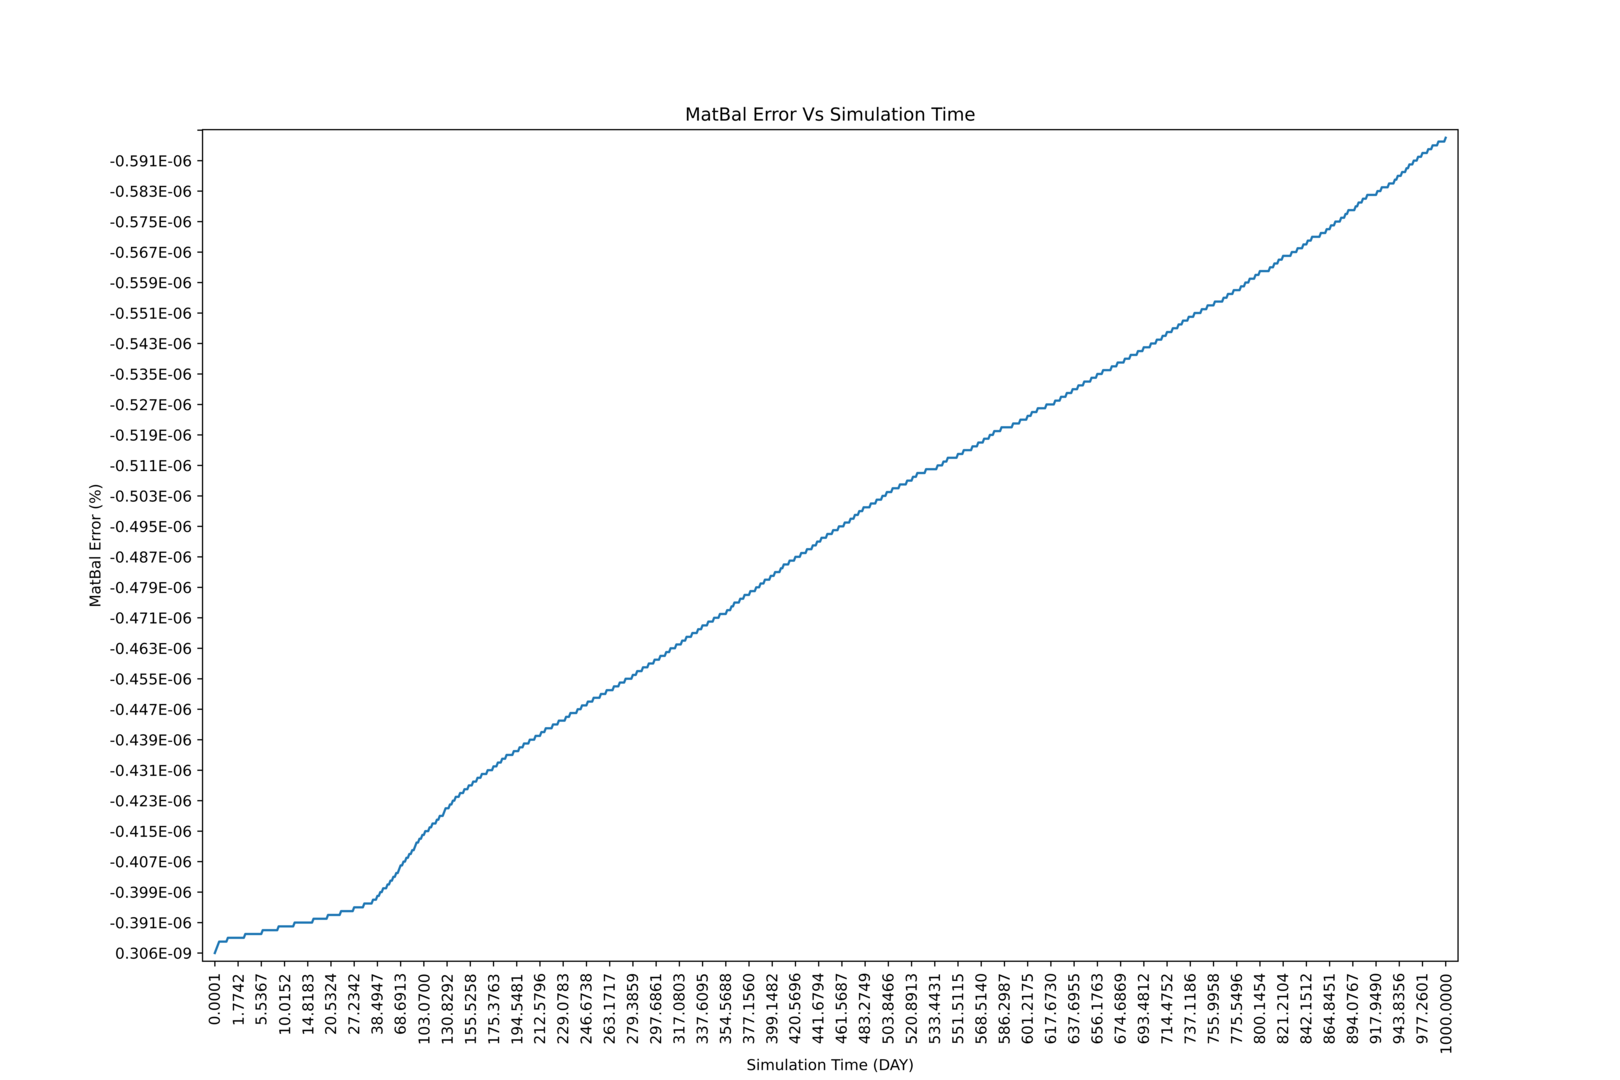
\includegraphics[width=1.1\linewidth]{figures/case8/cpr/matbalerr_time.png_reduced.png}
  \caption{\texttt{CPR-AMG} preconditioner.}
	\label{case8_matbalerr_cpr}
\end{subfigure}%
\begin{subfigure}{.5\textwidth}
  \centering
  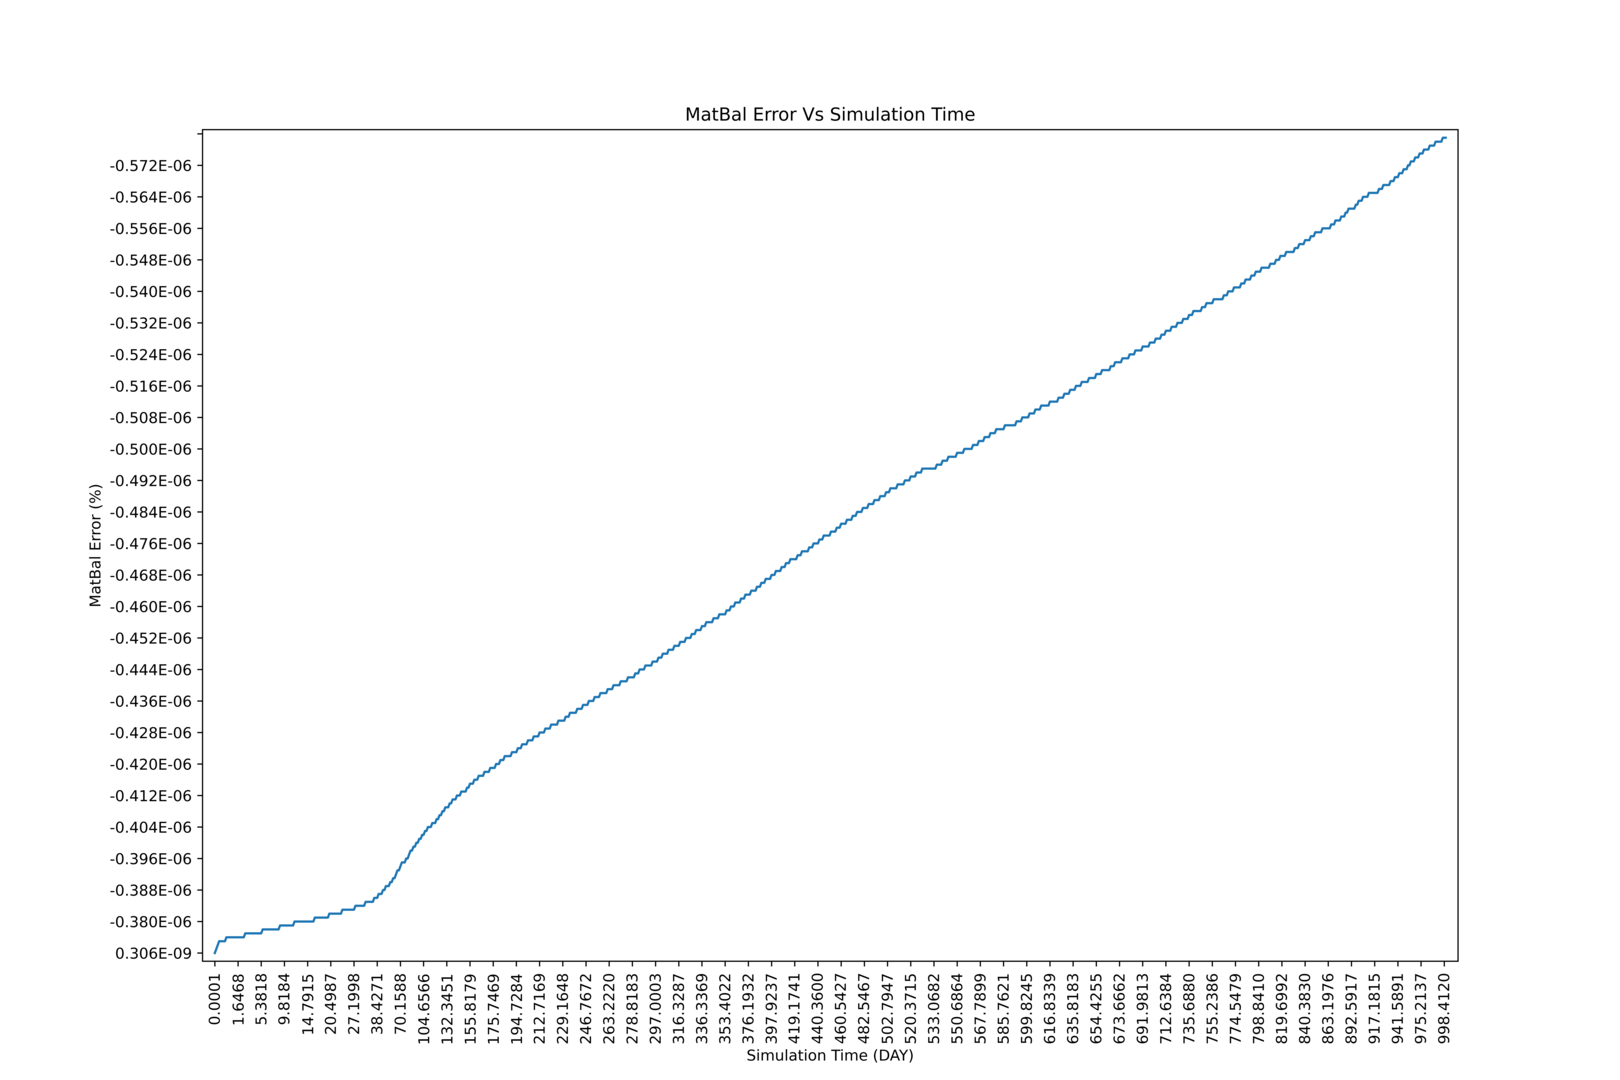
\includegraphics[width=1.1\linewidth]{figures/case8/ilu/matbalerr_time.png_reduced.png}
  \caption{\texttt{GMRES-ILU(0)} preconditioner}
	\label{case8_matbalerr_ilu}
\end{subfigure}
\caption[caption]{A comparison for \texttt{Case 4} for the two different preconditioning methods.\\\hspace{\textwidth}
		\cref{case8_cpu_cpr,case8_cpu_ilu}: CPU run time against simulation time. \\\hspace{\textwidth}
		\cref{case8_its_cpr,case8_its_ilu}: Linear iterations against simulation time.\\\hspace{\textwidth}
		\cref{case8_matbalerr_cpr,case8_matbalerr_ilu}: Material balance error against simulation time.}
\label{case8sg}
\end{figure}
\clearpage

\section{Case 5}
This model is simillar to the previous case instead of flooding with water, gas is used instead. Parameters of the reservoir
are the same as the previous case \ref{case4}.

\begin{table}[h!]
   \caption{Comparison parameters for \texttt{Case 5}.}
   \label{case5-tab}
   \small
   \centering
   \begin{tabular}{lcc}
   \toprule\toprule
   \textbf{Variable} & \textbf{CPR-AMG} & \textbf{GMRES-ILU(0)} \\
   \midrule
   CPU Time (hr) & 64.25 &  71.9 \\
   Solver Time (hr) & 49 & 56.9 \\
   \# Newton Iterations & 11,104 & 11,029 \\
   \# Solver Iterations & 92,218 & 376,594 \\
   \# Time Steps & 4,740 & 4,735 \\
   \bottomrule
   \end{tabular}
\end{table}

\begin{figure}[h!]
\centering
\begin{subfigure}{.5\textwidth}
  \centering
  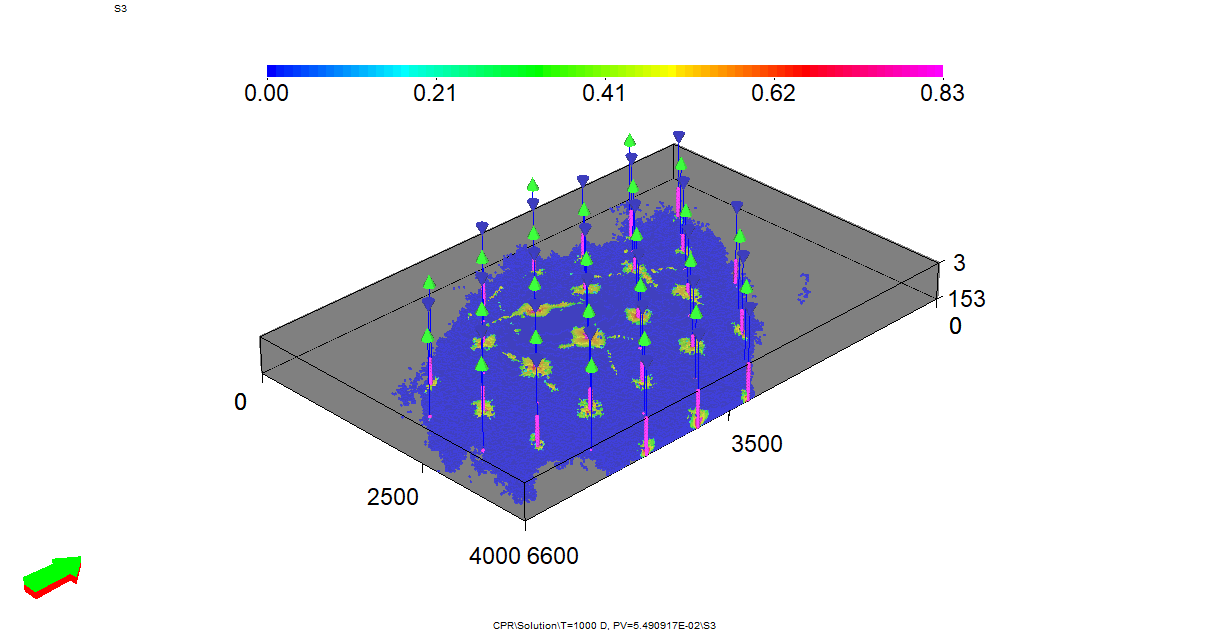
\includegraphics[width=1.3\linewidth]{figures/Case9_CPR_Sg.png}
  \caption{\texttt{CPR-AMG} preconditioner.}
\end{subfigure}%
\begin{subfigure}{.5\textwidth}
  \centering
  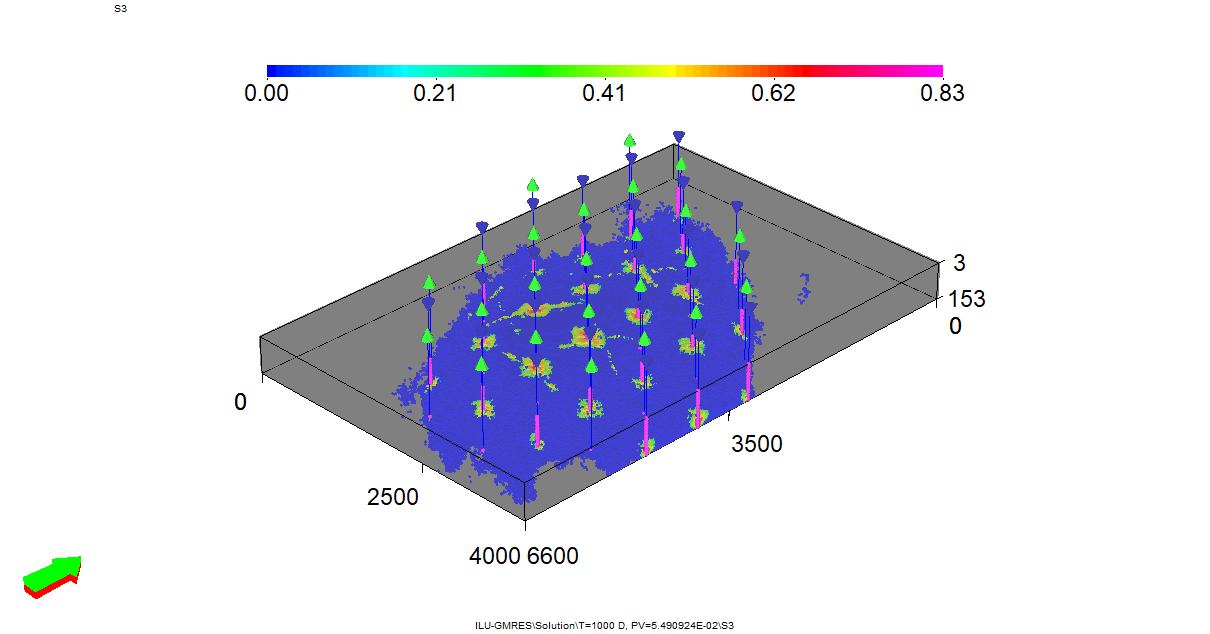
\includegraphics[width=1.3\linewidth]{figures/Case9_ILU-GMRES_Sg.png}
  \caption{\texttt{GMRES-ILU(0)} preconditioner}
\end{subfigure}
\caption{A comparison of \texttt{Case 5} gas saturation $S_{g}$ distribution for the two different preconditioning methods after 1000days of simulation.}
\label{case5sg}
\end{figure}

\begin{figure}
\centering
\begin{subfigure}{.5\textwidth}
  \centering
  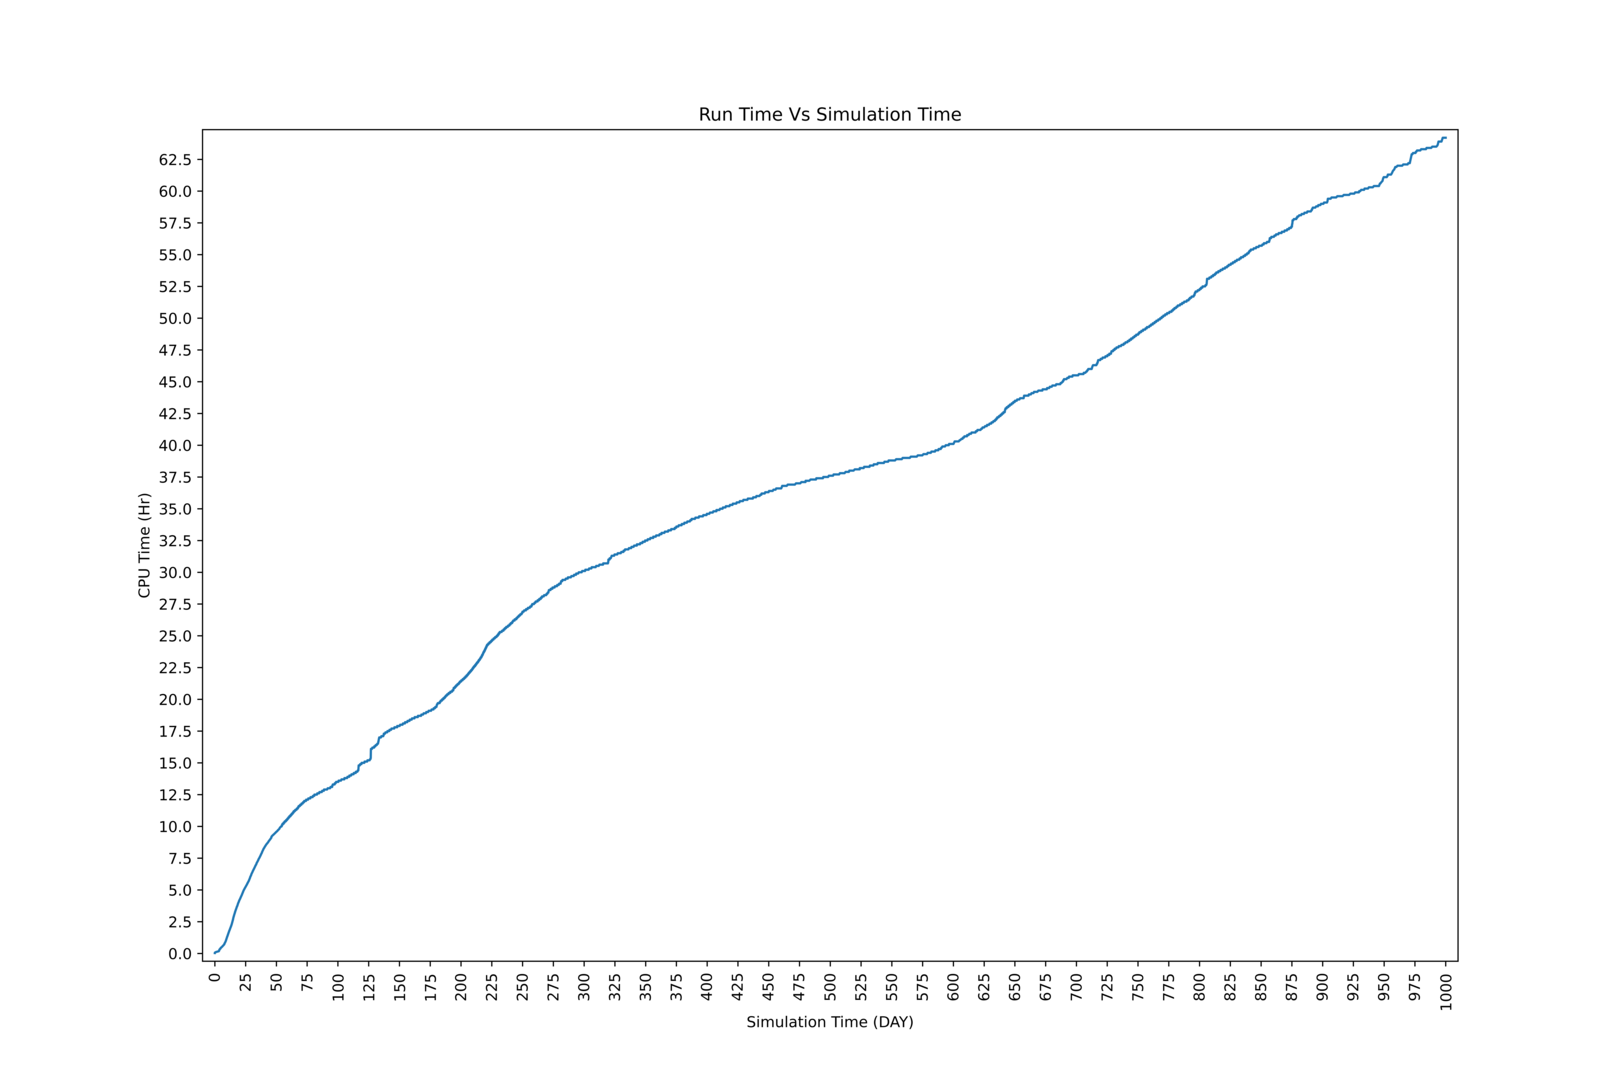
\includegraphics[width=1.1\linewidth]{figures/case9/cpr/cpu_time.png_reduced.png}
  \caption{\texttt{CPR-AMG} preconditioner.}
	\label{case9_cpu_cpr}
\end{subfigure}%
\begin{subfigure}{.5\textwidth}
  \centering
  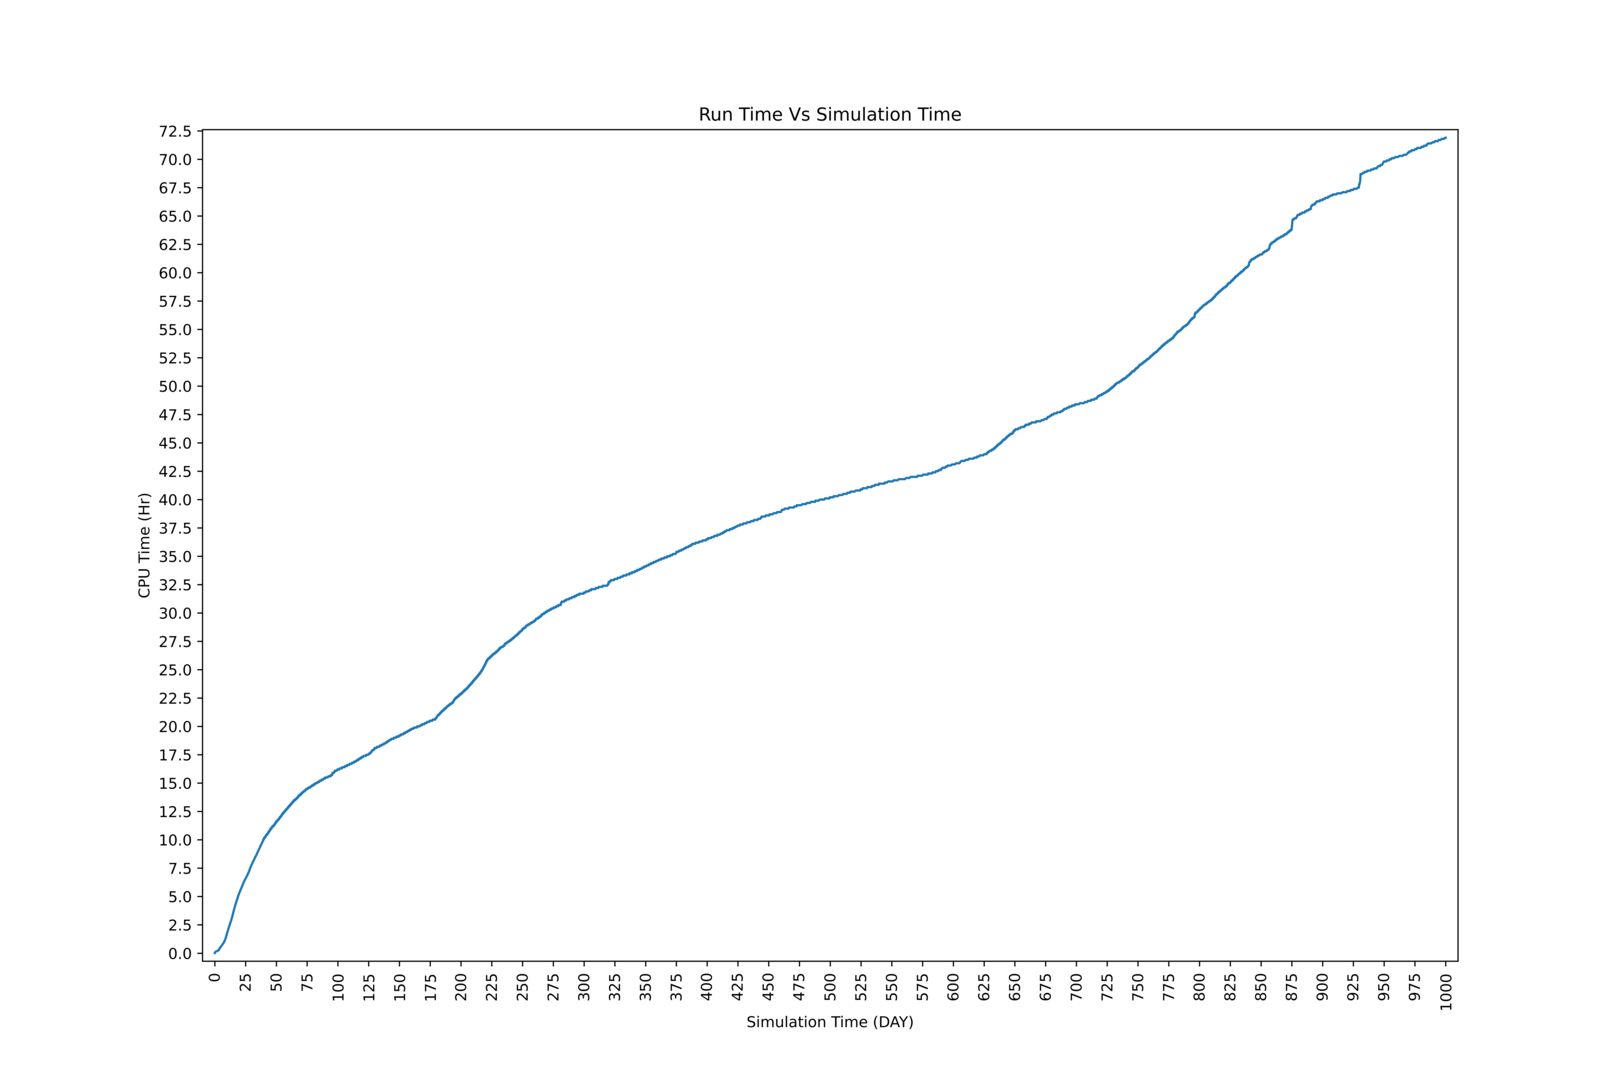
\includegraphics[width=1.1\linewidth]{figures/case9/ilu/cpu_time.png_reduced.png}
  \caption{\texttt{GMRES-ILU(0)} preconditioner}
	\label{case9_cpu_ilu}
\end{subfigure}
\begin{subfigure}{.5\textwidth}
  \centering
  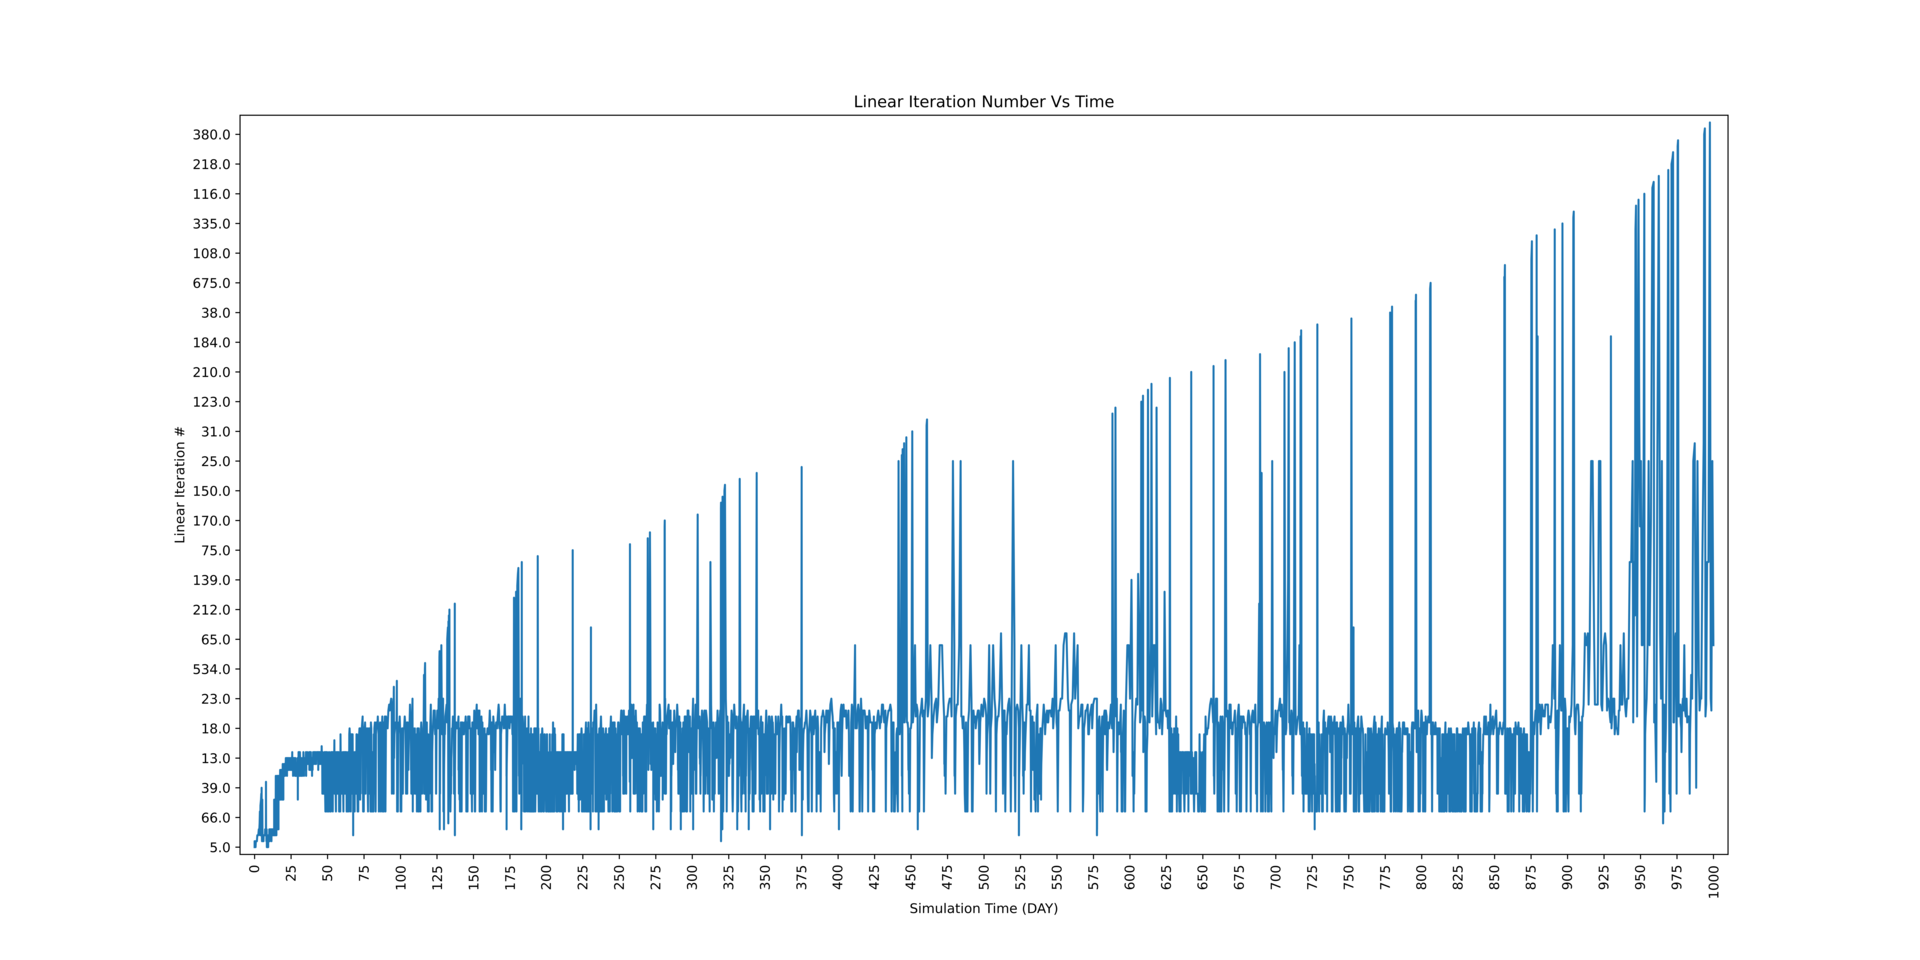
\includegraphics[width=1.1\linewidth]{figures/case9/cpr/its_time.png_reduced.png}
  \caption{\texttt{CPR-AMG} preconditioner.}
	\label{case9_its_cpr}
\end{subfigure}%
\begin{subfigure}{.5\textwidth}
  \centering
  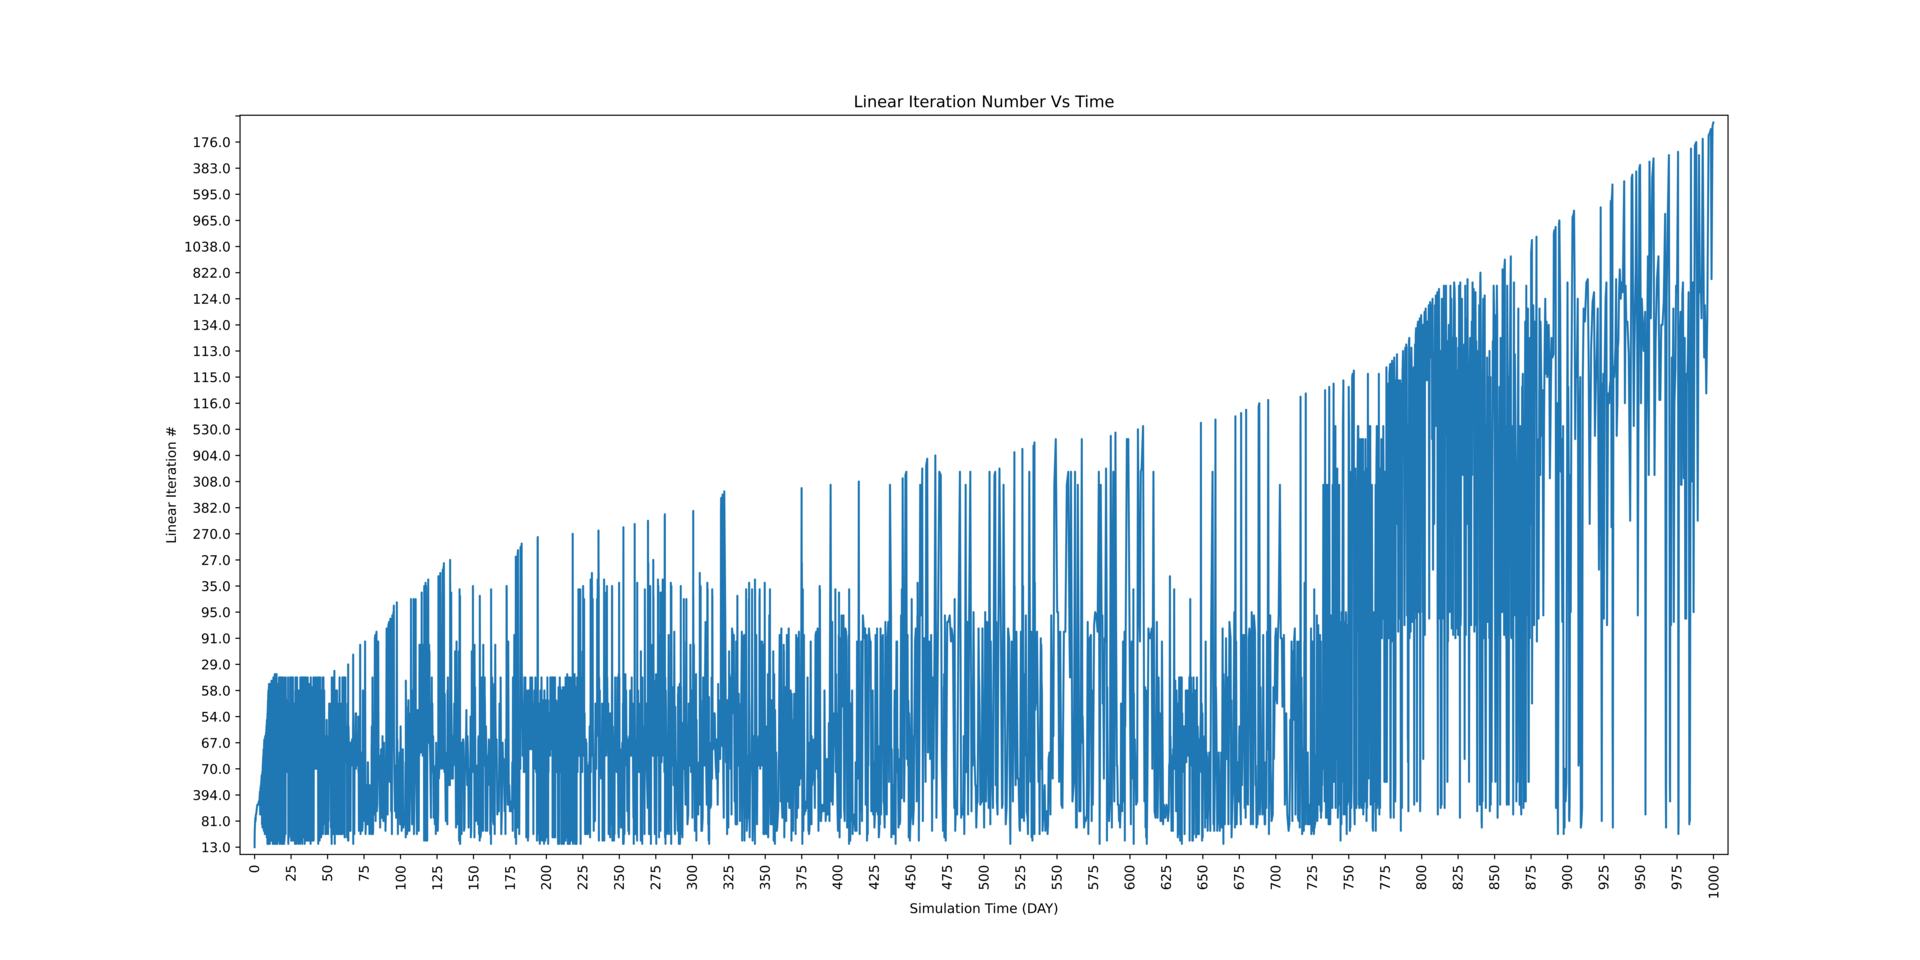
\includegraphics[width=1.1\linewidth]{figures/case9/ilu/its_time.png_reduced.png}
  \caption{\texttt{GMRES-ILU(0)} preconditioner}
	\label{case9_its_ilu}
\end{subfigure}
\begin{subfigure}{.5\textwidth}
  \centering
  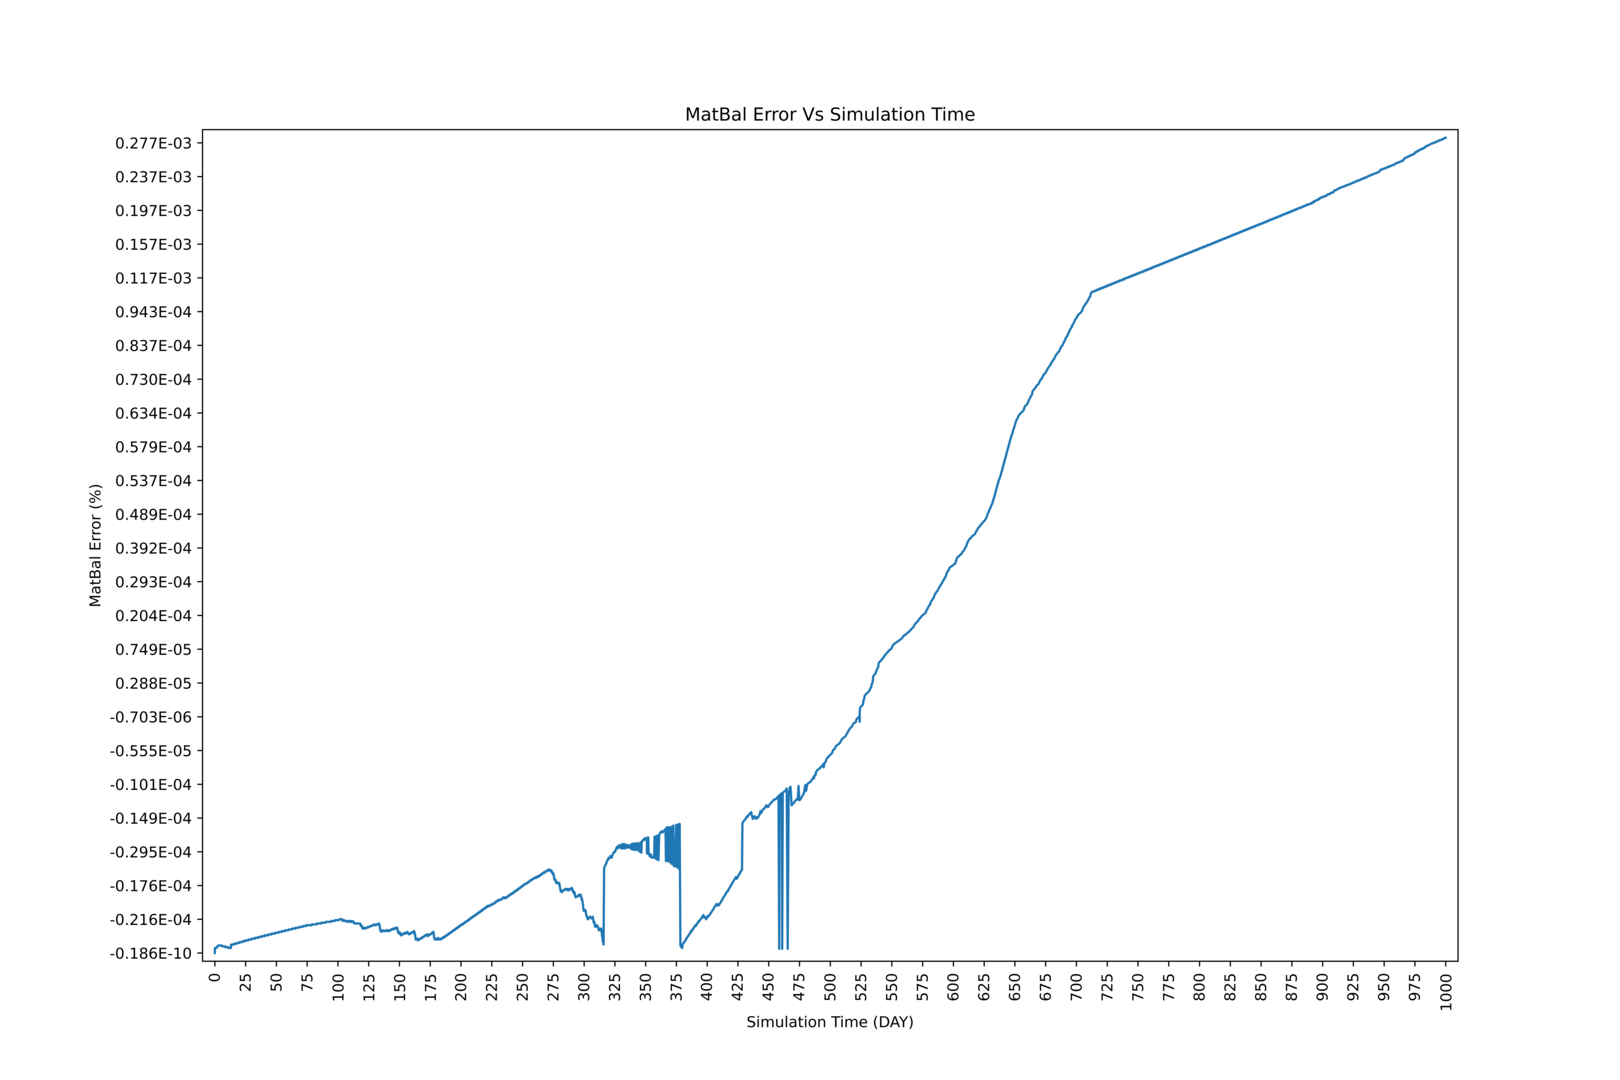
\includegraphics[width=1.1\linewidth]{figures/case9/cpr/matbalerr_time.png_reduced.png}
  \caption{\texttt{CPR-AMG} preconditioner.}
	\label{case9_matbalerr_cpr}
\end{subfigure}%
\begin{subfigure}{.5\textwidth}
  \centering
  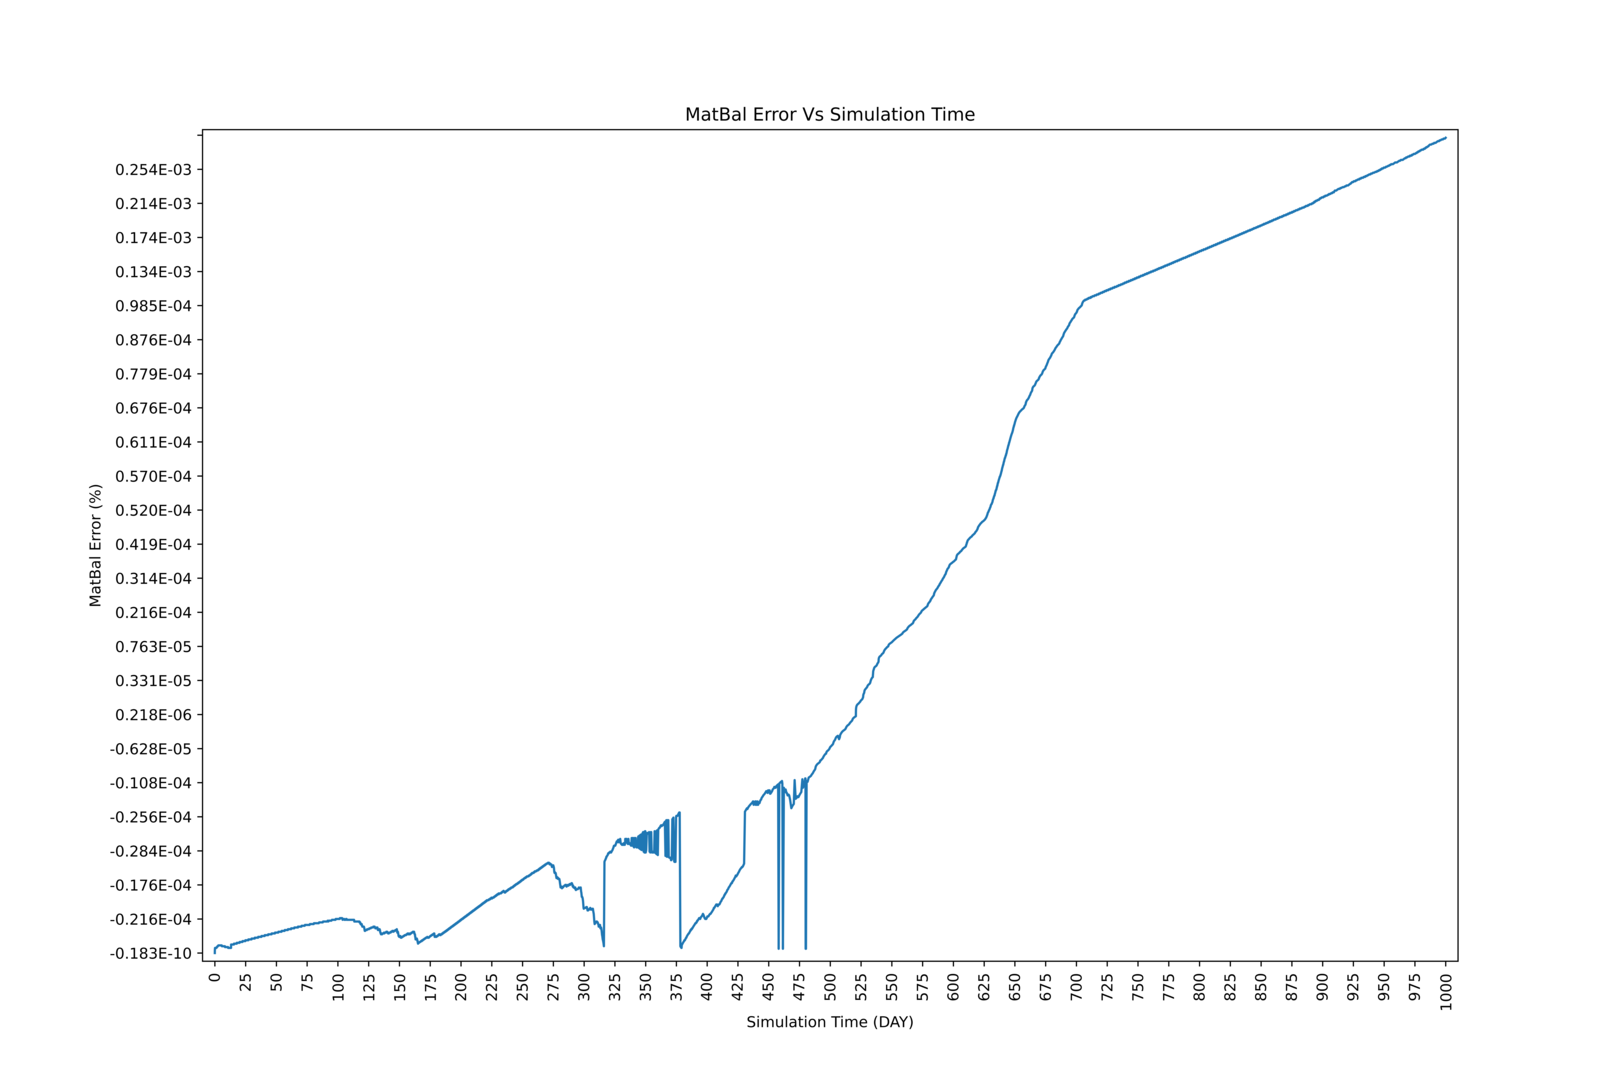
\includegraphics[width=1.1\linewidth]{figures/case9/ilu/matbalerr_time.png_reduced.png}
  \caption{\texttt{GMRES-ILU(0)} preconditioner}
	\label{case9_matbalerr_ilu}
\end{subfigure}
\caption[caption]{A comparison for \texttt{Case 5} for the two different preconditioning methods.\\\hspace{\textwidth}
		\cref{case9_cpu_cpr,case9_cpu_ilu}: CPU run time against simulation time. \\\hspace{\textwidth}
		\cref{case9_its_cpr,case9_its_ilu}: Linear iterations against simulation time.\\\hspace{\textwidth}
		\cref{case9_matbalerr_cpr,case9_matbalerr_ilu}: Material balance error against simulation time.}
\label{case9sg}
\end{figure}
\clearpage

\section{Case 6}
This simulation model is a modified version of a study of how compositional effects contribute to oil displacement by CO$_{2}$\supercite{case6paper}.
The modification is done to investigate grid refinement. The simulation grid was refined to $20\times20$, $80\times80$ and $320\times320$.
The heterogeneity of porosity and permeability were altered from those published in the paper to allow for viscous fingering.
This simulation problem was the most intresting case for the CPR preconditioner, since the default \texttt{ILU(0)-GMRES} solver-preconditioner combination
could not finish the simulation in less than a day for the ($320\times320$) scenario, when CPR managed to finish it within 12.68 hours. 

\FloatBarrier
\begin{center}
\begin{table}[h!]
\begin{adjustbox}{width=0.5\textwidth}
    \begin{threeparttable}
    \caption{\textbf{Case 4 Reservoir Parameters\supercite{phdfernandes}.}}
    \label{case4}
        \begin{tabular}{l r }
            \toprule
            Simulatoin Parameters & Value\\
            \midrule
	\rowcolor{red!20}\textit{\textbf{Reservoir data}}      & \\
	Grid:      &            \\
	\rowcolor{blue!5}Number of wells:      &  2 (1 injector / 1 producer) \\
	Length, width and thickness:      & \\
	\rowcolor{blue!5}Porosity:       &           \\
	Permeability ($X, \ Y, \ Z$) &  mD\\
	\rowcolor{blue!5}Initial water saturation:    &  \\      
	Formation temperature:    &  F$^{\circ}$     \\
	\rowcolor{blue!5}Initial pressure:    &       psi\\
	Reservoir’s initial composition () & \\
        \bottomrule
        \end{tabular}
    \end{threeparttable}
\end{adjustbox}    
\end{table}
\end{center}
\FloatBarrier

\begin{table}[h!]
   \caption{Comparison parameters for \texttt{Case 6}.}
   \label{case6-tab}
   \small
   \centering
   \begin{tabular}{lcc}
   \toprule\toprule
   \textbf{Variable} & \textbf{CPR-AMG} & \textbf{GMRES-ILU(0)} \\
   \midrule
   CPU Time (hr) & 12.67 &  NA \\
   Solver Time (hr) & 7.2  & NA \\
   \# Newton Iterations & 14,695 & NA\\
   \# Solver Iterations & 167,070 & NA \\
   \# Time Steps & 4,011& NA \\
   \bottomrule
   \end{tabular}
\end{table}

\begin{figure}[h!]
\centering
\begin{subfigure}{.5\textwidth}
  \centering
  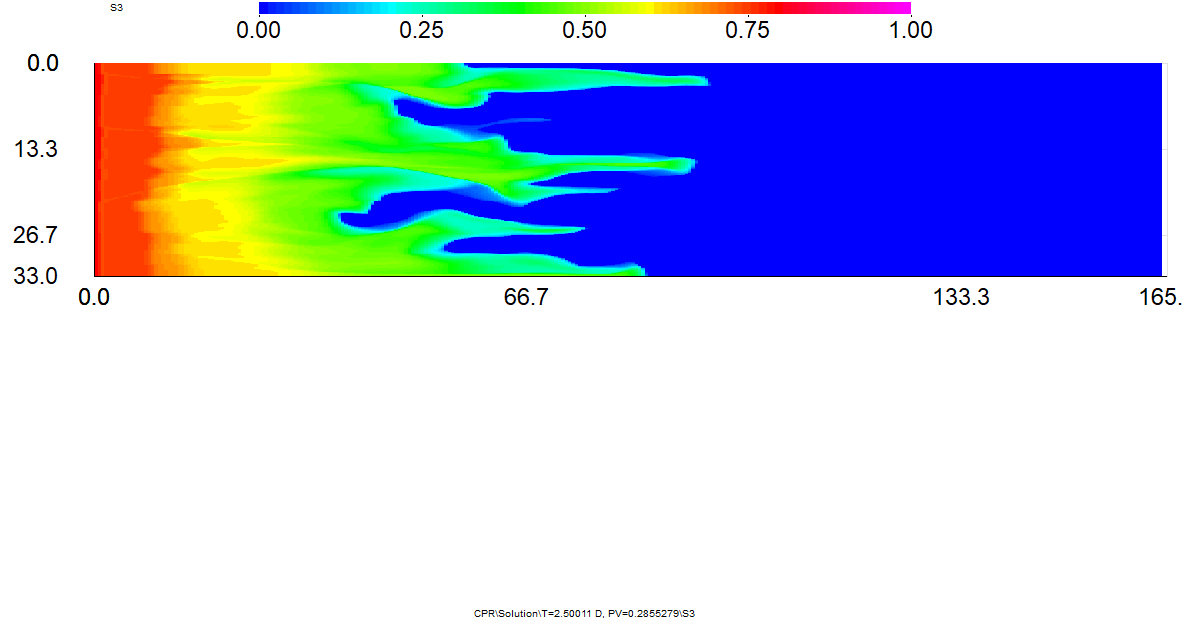
\includegraphics[width=1\linewidth]{figures/case6_cpr_sg.png}
  \caption{\texttt{CPR-AMG} preconditioner.}
\end{subfigure}%
\begin{subfigure}{.5\textwidth}
  \centering
  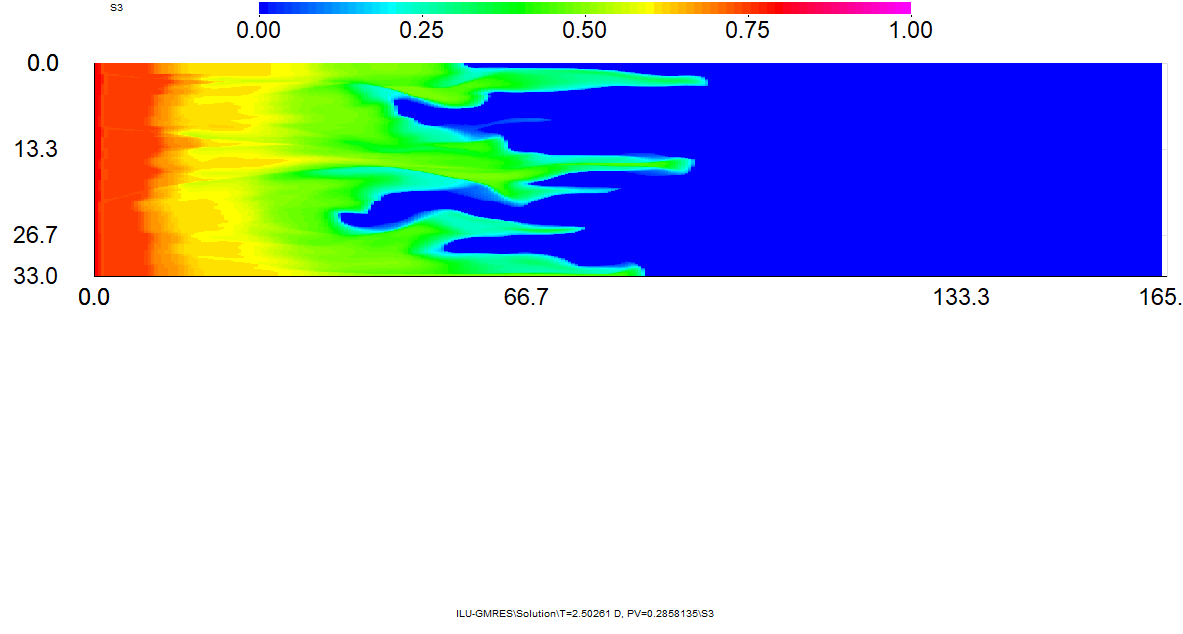
\includegraphics[width=1\linewidth]{figures/case6_ilu_sg.png}
  \caption{\texttt{GMRES-ILU(0)} preconditioner}
\end{subfigure}
\caption{A comparison of \texttt{Case 6} gas saturation $S_{g}$ distribution for the two different preconditioning methods after 2.5 days of simulation time.}
\label{case5sg}
\end{figure}

\begin{figure}[h!]
\centering
\begin{subfigure}{.5\textwidth}
  \centering
  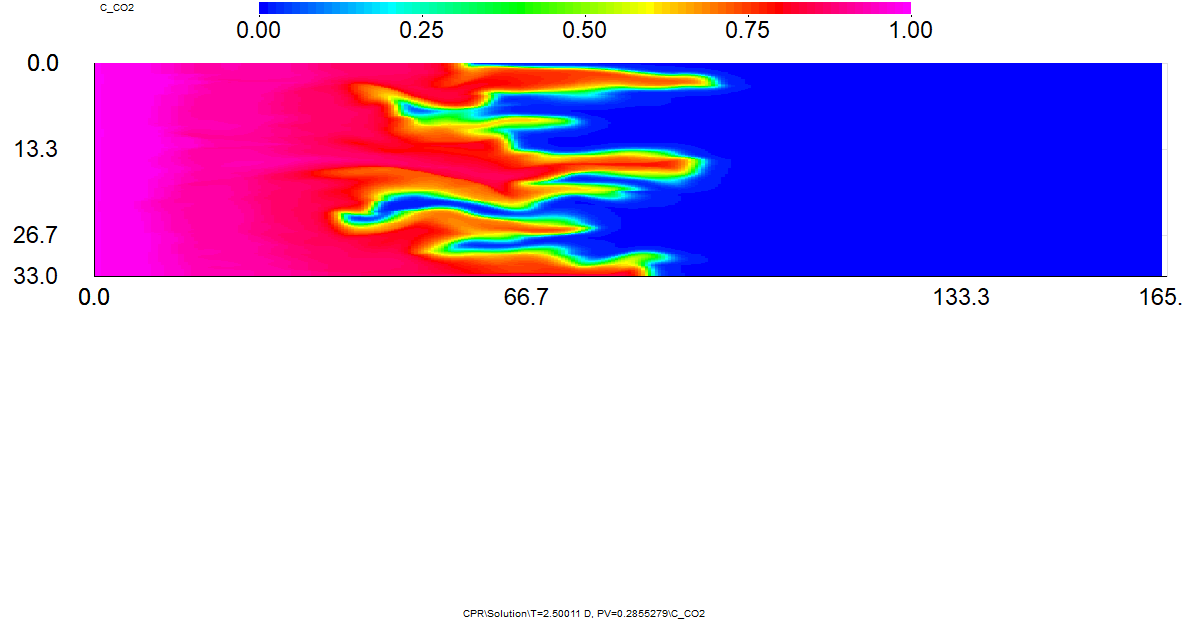
\includegraphics[width=1\linewidth]{figures/case6_cpr_co2.png}
  \caption{\texttt{CPR-AMG} preconditioner.}
\end{subfigure}%
\begin{subfigure}{.5\textwidth}
  \centering
  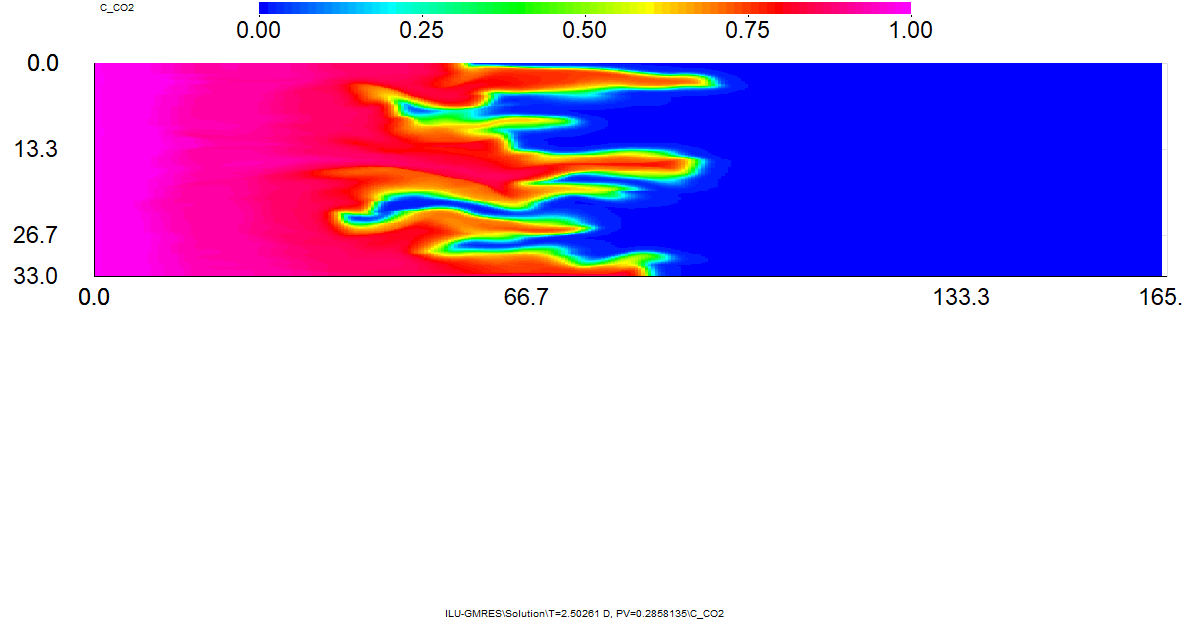
\includegraphics[width=1\linewidth]{figures/case6_ilu_co2.png}
  \caption{\texttt{GMRES-ILU(0)} preconditioner}
\end{subfigure}
\caption{A comparison of \texttt{Case 6} CO$_{2}$ saturation $S_{g}$ distribution for the two different preconditioning methods after 2.5 days of simulation time.}
\label{case5sg}
\end{figure}

